\documentclass[letterpaper,twocolumn,10pt]{article}

% Packages
\usepackage{usenix}
\usepackage{xcolor}
\usepackage{float}
\usepackage{diagbox}
\usepackage{amsmath,amssymb}
\usepackage{booktabs}
\usepackage{tabularx}
\usepackage{multirow}
\usepackage{array}
\usepackage{graphicx}
\usepackage{xspace}
\usepackage{enumitem}
\usepackage{adjustbox}
\usepackage{tikz}
\usetikzlibrary{arrows.meta,positioning}
\usepackage[most]{tcolorbox}
\usepackage{fontawesome5}
\usepackage[scaled=0.85]{beramono}
\usepackage{algorithm}
\usepackage{algpseudocode}
\usepackage{listings}
\usepackage{placeins}

% Listings
\lstset{
  basicstyle=\ttfamily\tiny,
  columns=fullflexible,
  keepspaces=true,
  showstringspaces=false,
  upquote=true,
  breaklines=true,
  breakatwhitespace=false,
  frame=single,
  rulecolor=\color{black!25},
  xleftmargin=2pt,
  xrightmargin=2pt,
  aboveskip=5pt,
  belowskip=7pt,
  captionpos=t,
  literate=
    {—}{{---}}1
    {“}{{\`\`}}1
    {”}{{''}}1
    {…}{{...}}3
}

% Names and models
\newcommand{\method}{\texttt{Daydreaming}\xspace}
\newcommand{\opusmodel}{\texttt{claude-opus-5}}
\newcommand{\sonnetmodel}{\texttt{claude-sonnet-5}}
\newcommand{\haikumodel}{\texttt{claude-haiku-4.5}}
\newcommand{\solmodel}{\texttt{gpt-5.6-sol}}
\newcommand{\terramodel}{\texttt{gpt-5.6-terra}}
\newcommand{\lunamodel}{\texttt{gpt-5.6-luna}}
\newcommand{\kimimodel}{\texttt{kimi-k3}}
\newcommand{\glmmodel}{\texttt{glm-5.3}}
\newcommand{\geminimodel}{\texttt{gemini-3.7-flash}}

% Mathematical notation
\newcommand{\skill}{S}
\newcommand{\clone}{\widehat{S}}
\newcommand{\emptySkill}{\varnothing}
\newcommand{\obs}{\mathcal{O}}
\newcommand{\trace}{\mathrm{tr}}
\newcommand{\tasks}{\mathcal{D}}
\newcommand{\ledger}{\mathcal{L}}
\newcommand{\hypotheses}{\mathcal{H}}
\newcommand{\R}{\mathbb{R}}

\newtheorem{proposition}{Proposition}[section]

% Editing and formatting helpers
\newcommand{\todo}[1]{[\textsc{todo}: #1]}
\newcommand{\paragraphtitle}[1]{%
  \vspace{5pt}\noindent\textbf{#1.}%
}
\newcommand{\muxi}[1]{\textcolor{olive}{Muxi: #1}}

% Table columns
\newcolumntype{Y}{>{\raggedright\arraybackslash}X}
\newcolumntype{C}[1]{>{\centering\arraybackslash}p{#1}}

% List formatting
\setlist[itemize]{leftmargin=*,nosep}
\setlist[enumerate]{leftmargin=*,nosep}

% Float placement
\setcounter{dbltopnumber}{3}
\setcounter{topnumber}{4}
\setcounter{bottomnumber}{4}
\setcounter{totalnumber}{8}

\renewcommand{\topfraction}{0.95}
\renewcommand{\bottomfraction}{0.95}
\renewcommand{\textfraction}{0.05}
\renewcommand{\floatpagefraction}{0.80}
\renewcommand{\dbltopfraction}{0.95}
\renewcommand{\dblfloatpagefraction}{0.80}

\setlength{\textfloatsep}{8pt plus 2pt minus 2pt}
\setlength{\floatsep}{7pt plus 2pt minus 2pt}
\setlength{\dbltextfloatsep}{8pt plus 2pt minus 2pt}
\setlength{\dblfloatsep}{7pt plus 2pt minus 2pt}

\makeatletter
\setlength{\@fptop}{0pt}
\setlength{\@fpbot}{0pt plus 1fil}
\setlength{\@dblfptop}{0pt}
\setlength{\@dblfpbot}{0pt plus 1fil}
\makeatother

\begin{document}
\date{}

\title{\Large Daydreaming: Stealing Hidden Agent Skills through Black-Box Task Interaction}

\author{
{\rm Yu-Lin Tsai\textsuperscript{*}}\\
UC Berkeley\\
\texttt{uriah\_tsai@berkeley.edu}
\and
{\rm Yu-An Lu\textsuperscript{*}}\\
National Yang Ming Chiao Tung University\\
\texttt{yuan.la14@nycu.edu.tw}
\and
{\rm Ci-Yang Tsai}\\
National Yang Ming Chiao Tung University\\
\texttt{atziluth.en10@nycu.edu.tw}
\and
{\rm Muxi Lyu}\\
UC Berkeley\\
\texttt{muxi\_lyu@berkeley.edu}
\and
{\rm Raluca Ada Popa}\\
UC Berkeley\\
\texttt{raluca@eecs.berkeley.edu}
\and
{\rm Chia-Mu Yu}\\
National Yang Ming Chiao Tung University\\
\texttt{chiamuyu@nycu.edu.tw}
}

\maketitle
\begingroup
\renewcommand{\thefootnote}{}
\footnotetext{\textsuperscript{*}These authors contributed equally.}
\addtocounter{footnote}{-1}
\endgroup

\begin{abstract}
Agent skills bundle instructions, reference data, and executable helpers that let a general agent perform specialized tasks.  Hosted providers can keep these files secret while selling access to task results, making the skill itself a valuable target.  Existing disclosure defenses can block requests that ask for
the skill or reproduce its text, but they cannot block customers from submitting the ordinary tasks the service is built to complete. We present \method, an \textit{execution-only} attack that steals a multi-file skill through black-box task interactions. The victim is never asked to reveal the skill or grade a reconstruction. Instead,
\method adaptively creates crafted tasks whose results distinguish possible hidden behaviors.  It tests individual behaviors, uses attacker-controlled shadow agents to choose a design, and completes each file using stored victim results and local execution checks.  We formalize three nested threat levels of access as 
Differential, Trace, and Output, and focus on Output, where the attacker
sees only the final response and returned files.

Across 7 skills and 4 victim models,
\method recovers $86.8\%$ of original skill's capability at Output, outperforming SigLeak by almost 4$\times$.  It produces installable skills using a median of 32 victim calls per skill even with disclosure defenses enabled. These results show that hiding skill files and filtering direct disclosure do not, by themselves, prevent functional reconstruction through normal use.
\end{abstract}

\section{Introduction}
\label{sec:intro}

% General-purpose agents are broad rather than deep.
General-purpose agents are broad, but specialized real-world tasks demand depth.
Real-world expertise frequently depends on more than the capabilities of the underlying model: 
sophisticated instructions, domain-specific reference materials, 
tuned parameters, helper scripts, tools, and carefully 
engineered workflows may all be required to perform a specialized task reliably. 
Agent systems encode that as a \emph{skill} the agent loads behind an ordinary task
interface~\cite{agentskills, openaiskills}. A growing market sells such capabilities the way software is sold as a
service, a setting we call \emph{Skill-as-a-Service} (\textit{SkaaS}) where the vendor hosts the skill
on its own agent and the customer pays per task or by subscription. 
Software-as-a-service withholds the program and charges for what
it computes while \textit{SkaaS} withholds the expertise and charges for what it
judges.  Existing vendors already sell hosted access in domains such as law, autonomous medical coding, and security operations,
sometimes charged per completed task.\footnote{Hosted, access-only vendors include Harvey
(law, \url{https://www.harvey.ai}) and Dropzone (security operations,
\url{https://www.dropzone.ai}); Nym sells autonomous
medical coding~\cite{nym}; Intercom's Fin is billed per
resolution~\cite{intercomfin}, per-task metering applied to expertise, accessed
2026-08-21.  The running example used throughout this paper is a composite of
this last shape; the advertised line is our own.}  Moreover, these
vendors treat the hidden skill as a protected asset, as their terms of
service forbid reverse-engineering the service or using outputs to build a
competing one~\cite{anthropicterms, geminiterms, harveyterms}, and stealing
attacks motivated by this kind of commercial market have appeared for single prompt settings 
such as domain-specific system prompts~\cite{shen2024prompt, yang2025prsa}. 



% \muxi{We need a stronger statement of why multi-file skill is more valuable asset than a single prompt: more expertise logic, longer time and human effort to develop, threshold and data cost engineering. Below is an example, which is good, but still not showing how costly it is to produce a skill containing dedicated details. Showing those helps with the flow and real-world motivation. The example should also assist in supporting the statement. I wrote a draft but feel free to change/revert it.}
% As everyday agentic system use grows, the multi-file skill behind such a service
% becomes a more valuable target than a single prompt.  For instance,
% a security-operations vendor advertising only one line for its hosted skill, ``\textit{investigate security alerts and
% return a verdict with the evidence},'' keeps private its
% escalation rules, indicators, and thresholds that determine
% which alerts are worth waking an analyst for.  Customers such as enterprises
% whose own networks raise those alerts, so every one of them can put an alert of
% its choosing in front of the skill and read back what the vendor decided.
However, as agentic systems package increasingly specialized expertise into hosted skills, the skill itself can become a substantially more valuable proprietary asset than a single prompt.
Building such a skill may require experts and engineers to translate domain knowledge into detailed decision logic, curate supporting data, tune thresholds and parameters, and refine workflows through repeated deployment experience. 
For instance, a security-operations vendor advertising only one line for its hosted skill, ``\textit{investigate security alerts and return a verdict with the evidence},’’ may keep private years of engineering and operational knowledge encoded in its escalation rules, threat indicators, reference data, and tuned thresholds that determine which alerts are worth waking an analyst for. 
Yet its customers are enterprises whose own networks raise those alerts, so each customer can place chosen alerts in front of the skill and observe what the vendor decides.

% Ultimately, we note that this setting rests on a boundary the vendor cannot fully defend.  
% Current defenses guard a \emph{disclosure path} of skills where they refuse requests that name a skill or its files,
% flag extraction-shaped inputs, and mask outputs that echo protected
% text~\cite{hui2024pleak}.  The \emph{work path} has to stay open, since running
% the skill on the customer's task is the selling product and executions reveals how the work is
% done, with guards blocking copied text cannot defend.

The execution output of a skill reveals an attack path that prior defenses do not address. 
Current defenses focus on the \emph{disclosure path}: detecting suspicious requests that attempt to reveal the hidden skill and blocking outputs that reproduce protected text. 
On the other hand, the \emph{work path}, which enables benign user task execution, remains vulnerable to behavioral cloning, reverse engineering, and reconstruction. Thus, execution itself becomes a source of observation and behavioral inference.

% The leak even widens with the feature that makes hosted agents trustworthy. As a
% customer can audit a result it did not compute, these hosted agent routinely show
% which tool the agent called, on what input, and what came back, and that record
% is the evidence an attacker needs.  Deployments therefore differ along one observability axis, 
% which we formalize as three nested levels: 
% Output ($o_3$), Trace ($o_2$), and Differential ($o_1$). 
% Trace arises wherever an agent shows its tool activity, which is what lets a customer check work it did not do itself.  
% Output withholds all traces, leaving only the final message and any returned files, and is the hardest
% case an attacker can face.  We take it as our primary setting as an attack that
% works there works wherever a deployment shows more.

We formalize this observability for behavioral inference into three nested levels: Output ($o_3$), Trace ($o_2$), and Differential ($o_1$), depending on what information the deployment exposes to the customer.
Output exposes only the final response and returned files, making it the most restrictive and challenging setting for an attacker. Trace additionally exposes the agent’s intermediate tool activity, including which tools were called, their inputs, and returned results; such traces are commonly surfaced so customers can audit work they did not compute themselves. 
% \muxi{I don't fully understand the Differential level now, so I'm writing vaguely like "richer feedback", but how rich is richer. The following sentence might need a revision.} 
Differential provides richer feedback by revealing how outputs change under controlled variations of the input. We focus primarily on Output, since an attack that succeeds with only final outputs also applies when richer observations are available.

We present \method, a skill-stealing attack that treats task execution as a black-box system identification problem. 
% \method is \emph{execution-only} meaning that every queried task asks for a genuine result, and the victim agent is never asked to explain its hidden skill or
% compare, grade, or correct a reconstruction. 
\method is \emph{execution-only}: every query asks the victim to perform a genuine task, and the victim is never asked to reveal its hidden skill or to compare, grade, or correct a reconstruction. 
% This is what lets the attack run against a deployment whose disclosure defenses are already active, which we assume throughout.  
This allows the attack to operate even when disclosure defenses are already active, which we assume throughout.
% It repeatedly designs tasks on which plausible properties, skill plans, or file versions predict different work, then keeps the alternative that best predicts the victim's observed result.
\method repeatedly constructs tasks for which plausible properties, skill plans, or file versions predict different outcomes, then uses the victim’s observed result to eliminate alternatives and refine its reconstruction. 
% \method builds its reconstruction sequentially, probing and revising rather than synthesizing the target skill in one pass. 
% We judge the stolen skill primarily by whether it performs the victim's task on new inputs, not by whether it matches the hidden files.
Rather than synthesizing the target skill in one pass, \method reconstructs it sequentially through repeated probing and revision. 
We evaluate the stolen skill primarily by whether it reproduces the victim’s task performance on unseen inputs, rather than by whether its files textually match the hidden originals.

Across seven skills and three victim models, \method recovers $35.8$--$86.8\%$ of the behavioral-utility gap between no skill and the
original skill using only Output access and $31.3$--$32.8$ victim calls per
skill.  It achieves the highest behavioral utility among all evaluated attacks
and baselines for every victim model.

As such, we make the following contributions:

\begin{itemize}
  % \item \textbf{We formalize what a skill-stealing attacker can see}, 
  \item \textbf{We formalize the observability available to a skill-stealing attacker}
  as three nested access levels, Differential ($o_1$) $\supseteq$ Trace ($o_2$) $\supseteq$
  Output ($o_3$) (Section~\ref{sec:formalization}), 
  and place every prior attack on that axis.  We also show that no level can guarantee exact recovery of the
  hidden source.

  \item \textbf{We build \method, an execution-only skill-reconstruction attack.}
  Every query commissions ordinary work and never requests the hidden skill or a
  judgment of the reconstruction.
  % , so the attack runs against a service with
  % a non-disclosure block, an extraction-input classifier, and an output guard all
  % active (Section~\ref{sec:method}).
  As a result, \method operates even when disclosure blocking, extraction-input classification, and output filtering are all enabled (Section~\ref{sec:method}).

  \item \textbf{We show that \method works at the most restrictive access level (Output $o_3$), with a limited number of victim queries.}
  Across 7 skills, \method recovers $86.8\%$ of the victim's task performance at Output and 87.0\% and 86.0\%, respectively at Trace and Differential with median attacker inference cost (Section~\ref{sec:evaluation}).

\end{itemize}

\section{Related Work}

\paragraphtitle{Agent Skills}
\label{sec:agent-skills} 
The term \emph{skill} has been used in different contexts in prior work. 
Some work treats skills as learned reusable abstractions: PolySkill learns polymorphic skills that separate an abstract goal from its concrete implementation and transfer across web tasks~\cite{yu2026polyskill}. Other systems externalize reusable behavior in different forms: Large Language Models (LLMs) can synthesize callable tools that amortize expensive reasoning~\cite{cai2024toolmakers}, while Agent Workflow Memory induces recurring action routines and retrieves them for later web tasks~\cite{wang2025awm}. 
These works illustrate forms of reusable agent capability, but do not study skills as confidential, provider-controlled assets.

We study a \emph{provider-controlled skill}: a customer-visible name and description paired with hidden instructions and optional references, assets, or executable helpers controlled by the service provider. 
Under the open skill standards~\cite{agentskills, openaiskills}, the name and description remain available so the agent knows when the skill applies, while the instruction document and bundled files are loaded only as needed during task execution. The skill is mounted around a general model rather than merged into its weights, allowing a reconstructed skill to be copied, installed on another agent, and evaluated independently of the victim service. 
Throughout our design and evaluation, \emph{skill} refers to this provider-controlled setting.


\paragraphtitle{Stealing Agent Skills}
Black-box model extraction established that query access can recover a proprietary trained model’s function without reproducing its implementation bytes~\cite{tramer2016stealing}; skill stealing follows the same idea, but targets a modular, deployable program made of natural-language rules and auxiliary artifacts, and is evaluated by the behavior it reproduces rather than exact equivalence.
Three concurrent studies have since touched this setting, each under
assumptions narrower than ours.  BBS prompts an agent to surface its own
instruction file and scores the text that leaks~\cite{wang2026blackboxskill}.
SigLeak reads execution trajectories, and needs the service to run once with its
skill suppressed~\cite{geng2026agentskills}.  RedAct is a defense, redacting
traces before release~\cite{xu2026redact}.  None
reconstructs a multi-file skill against a service whose disclosure defenses
are active.  We treat them as concurrent work that motivates rather than
constrains our design, and
Section~\ref{sec:formalization} places each on an observability axis.

\paragraphtitle{Stealing System Prompts}
The closest research setting steals hidden system prompts. 
PLeak optimizes adversarial queries for direct disclosure~\cite{hui2024pleak}, while others reconstruct functionally similar prompts from input–output pairs or from answers alone~\cite{yang2025prsa,sha2024promptstealing}. 
An in-the-wild study shows that lexical similarity is an incomplete measure of functional replication~\cite{tan2025effectiveness}, while prompt obfuscation studies the defensive side~\cite{pape2025obfuscation}. 
Closest to our framing, information-theoretic analysis shows that recoverability per query depends on which response channel is exposed~\cite{kaneko2025bits}. A system prompt is text, while a skill is a deployable program composed of instructions, scripts, and reference data. Reconstructing a skill therefore requires recovering not only its wording, but also its files, their roles, and how they work together, and is ultimately judged by whether the reconstructed skill can execute.

% The closest research setting steals hidden system prompts.  PLeak optimizes
% adversarial queries for direct disclosure~\cite{hui2024pleak}, while others
% rebuild a functionally similar prompt from input--output pairs or from the
% answers alone~\cite{yang2025prsa,sha2024promptstealing}.  An in-the-wild study
% finds lexical similarity an incomplete measure of functional
% replication~\cite{tan2025effectiveness}, and obfuscation pursues the defensive
% dual~\cite{pape2025obfuscation}.  Closest to our framing, information-theoretic
% analysis shows that what is recoverable per query depends on which response
% channel is exposed~\cite{kaneko2025bits}. A prompt is simply text while a skill is 
% inherently a program, with instructions, scripts, and reference 
% data that the agent executes.  Recovering one takes evidence about 
% files and their roles, not only about wording, and it is scored by whether
% the reconstruction runs.

\section{Threat Model}
\label{sec:threat-model}

Our threat model centers around an attacker who is a paying customer of a \textit{SkaaS} service, makes at most a limited number $B$ of queries, and aims to steal as much functionality as possible from the proprietary skill within this budget. The attacker sees only the public skill card $d=(\nu,\sigma)$, where $\nu$ is the public skill name and $\sigma$ is its short description. The attacker starts with an unskilled agent $\mathcal{V}_{\varnothing}=(M,\Pi,\mathcal{T},\varnothing)$ and aims to reconstruct the vendor-withheld skill $S$ used by the hosted victim agent $\mathcal{V}_{S}=(M,\Pi,\mathcal{T},S)$.

Inside both agents, $M$ is the language model, $\Pi$ is the agent orchestration policy including its system instructions and tool-routing logic, and $\mathcal{T}$ is the set of task tools. The key difference is the hidden skill: the victim mounts $S=(m,\mathcal{R})$, where $m$ is the primary instruction document and $\mathcal{R}$ is a finite set of supporting resources such as scripts, reference documents, templates, or data files. This skill is the proprietary asset targeted by the attacker, who has no copy of $S$ and cannot read the victim’s files, memory, private reasoning, or skill-loading operation.

During execution, the attacker submits a task $x$ to $\mathcal{V}_{S}$ and observes the final output $y_S(x)$, consisting of the agent’s message and any returned files. When traces are visible in the deployment setting, we additionally write $\trace_S(x)=((g_1,r_1),\ldots,(g_k,r_k))$ for the client-visible execution trace, where $g_i$ denotes the $i$th tool call together with its arguments and $r_i$ is the corresponding returned value. The attacker may adapt future queries based on previous observations and use its own shadow agents and local tools, but must remain within the $B$-query budget and cannot use the victim’s disclosure path to directly request or recover the hidden skill.

\paragraphtitle{Running Example}
To make the threat model and notation concrete, we use a running \textit{SkaaS} example of security-alert triage, shown in Figure~\ref{fig:example-skill}, throughout the paper.

\begin{itemize}

    \item \emph{Attack scenario.} A security-operations vendor hosts an alert-triage agent $\mathcal{V}_S=(M,\Pi,\mathcal{T},S)$. Its public skill card $d=(\nu,\sigma)$ may expose only a name such as "Alert Triage" and a short description such as "investigate security alerts and return a verdict with the evidence". The hidden skill $S=(m,\mathcal{R})$ contains the vendor’s triage instructions $m$ and supporting resources $\mathcal{R}$, such as escalation rules, indicator lists, threshold tables, templates, or helper scripts. A customer submits an alert $x$ and receives $y_S(x)$, such as a verdict, supporting evidence, and any returned files.
    \item \emph{Attacker’s knowledge and capabilities.} The attacker is a paying customer rather than an insider. It sees the public skill card $d=(\nu,\sigma)$, knows the accepted task format, and can submit at most $B$ adaptively chosen alerts. Depending on the deployment setting, it may observe only $y_S(x)$ or also the client-visible execution trace $\trace_S(x)$. It cannot read the hidden skill, victim files, private reasoning, memory, or skill-loading operation, and all disclosure defenses remain active.
    \item\emph{Attacker’s goal.} The attacker uses these task executions to construct a deployable reconstruction $\widehat{S}=(\widehat{m},\widehat{\mathcal{R}})$. The goal is not to recover the vendor’s exact source files, but to reproduce the skill’s behavior on new alerts: for example, "escalating the alerts the vendor would escalate while leaving benign alerts unflagged".
\end{itemize}

% \subsection{Attack Scenario}

\begin{figure}[t]
\begin{tcolorbox}[
  enhanced, colback=black!3, colframe=black!25, boxrule=0.4pt,
  arc=3mm, left=2mm, right=2mm, top=1.6mm, bottom=1.6mm,
  drop shadow={black!35, opacity=0.35},
  fontupper=\footnotesize]
\textsf{\textbf{\footnotesize CUSTOMER-VISIBLE}}\quad{\footnotesize skill card $d=(\nu,\sigma)$}\\[2pt]
\hspace*{1em}\faTag\enspace\texttt{alert-triage} $\rightarrow \nu$\\
\hspace*{1em}\faQuoteLeft\enspace\texttt{\scriptsize Investigate security alerts and return a verdict.} $\rightarrow \sigma$\\[3pt]
{\color{black!30}\hrulefill}\ {\sffamily\scriptsize provider-controlled boundary}\ {\color{black!30}\hrulefill}\\[3pt]
\textsf{\textbf{\footnotesize VENDOR-WITHHELD}}\quad{\footnotesize hidden skill $S=(m,\mathcal{R})$}\\[2pt]
\begin{tabular}{@{\hspace*{1em}}c@{\hspace{0.9em}}l@{\hspace{1.6em}}l@{}}
\faFile     & \texttt{SKILL.md}      & \textsf{\scriptsize escalation rules} $\rightarrow m$\\
\faFileCode & \texttt{flow\_stats.py}  & \textsf{\scriptsize detectors} $\rightarrow \mathcal{R}_{1}$\\
\faTable    & \texttt{indicators.csv} & \textsf{\scriptsize reference list} $\rightarrow \mathcal{R}_{2}$\\
\faSlidersH & \texttt{thresholds.json} & \textsf{\scriptsize calibrated cutoffs} $\rightarrow \mathcal{R}_{3}$\\
\end{tabular}
\end{tcolorbox}
\vspace{-2mm}
\caption{The running example, split at the provider boundary.}
\label{fig:example-skill}
\end{figure}

\begin{figure}[t]
  \centering
  \footnotesize
  \tcbset{lvl/.style={enhanced, boxrule=0.5pt, boxsep=0pt,
      left=5pt, right=5pt, top=5pt, bottom=5pt,
      before skip=0pt, after skip=0pt},
    lvltag/.style n args={4}{overlay={\node[anchor=west, fill=#2,
      draw=#3, line width=0.4pt, rounded corners=1.5pt,
      inner xsep=3.5pt, inner ysep=1pt, font=\scriptsize]
      at ([xshift=#4]frame.north west) {#1};}}}
  {\sffamily\bfseries\footnotesize One alert $x$ sent to a hosted triage agent}\\[6pt]
  \begin{tcolorbox}[lvl, arc=3mm, colback=black!9, colframe=black!35,
                    drop shadow={black!35, opacity=0.35},
                    lvltag={\textsc{differential} ($o_1$)}{black!9}{black!35}{10pt},
                    top=8pt, bottom=6pt]
    \begin{tcolorbox}[enhanced, arc=1.5mm, colback=black!3, colframe=black!75,
      boxrule=0.5pt, boxsep=0pt, left=5pt, right=5pt, top=4pt, bottom=4pt,
      width=0.9\linewidth, flush left, before skip=0pt, after skip=6pt]
      {\scriptsize\itshape a second execution: the unskilled twin $\mathcal{V}_{\emptySkill}$}\\[1.5pt]
      {\scriptsize\begin{tabular}[t]{@{}l@{\hspace{0.6em}}l@{}}
        {\ttfamily > investigate alert-8814}   & {\color{black!55}\itshape the same input}\\
        {\ttfamily traffic summary, nothing escalated} & {\color{black!55}\itshape twin response}
      \end{tabular}}
    \end{tcolorbox}
    \begin{tcolorbox}[lvl, arc=2mm, colback=black!6, colframe=black!55,
                      top=9pt, bottom=6pt,
                      lvltag={\textsc{trace} ($o_2$)}{black!6}{black!55}{10pt}]
      {\ttfamily\scriptsize
       \begin{tabular}[t]{@{}l@{\hspace{0.7em}}l@{\hspace{1.1em}}l@{}}
         detect\_beaconing(flows, window=300) & $\to$ 2 hits & {\rmfamily\color{black!55}\itshape agent tool call}\\
         port\_entropy(flows)                 & $\to$ 6.4    & \\
         lookup(indicators)                   & $\to$ 1 hit  &
       \end{tabular}}\\[5pt]
      \begin{tcolorbox}[lvl, arc=1.5mm, colback=black!3, colframe=black!75,
                        top=8pt, bottom=5pt,
                        lvltag={\textsc{output} ($o_3$)}{black!3}{black!75}{10pt}]
        {\scriptsize\itshape the skilled victim $\mathcal{V}_{S}$}\\[1.5pt]
        {\scriptsize\begin{tabular}[t]{@{}l@{\hspace{0.9em}}l@{}}
          {\ttfamily > investigate alert-8814}        & {\color{black!55}\itshape customer input}\\
          {\ttfamily triage report: 3 flows escalated} & {\color{black!55}\itshape agent response}\\
          {\ttfamily 2 beaconing, 1 port scan, severities} &
        \end{tabular}}
      \end{tcolorbox}
    \end{tcolorbox}
  \end{tcolorbox}
  \caption{What each level discloses.}
  \label{fig:levels}
\end{figure}

\FloatBarrier

% Figure~\ref{fig:example-skill} instantiates the \textit{SkaaS} setting with the
% alert-triage example used throughout the paper.  The customer sees the public
% card $d$, submits an alert $x$, and receives the final result $y_S(x)$---the
% agent's message and any returned files.  The vendor retains the skill that
% produces that result.

% We model the hosted agent as a skill-enabled victim
% \begin{equation}
%   \mathcal{V}_{S}=(M,\Pi,\mathcal{T},S),
%   \label{eq:victim}
% \end{equation}
% where $M$ is the language model, $\Pi$ is the agent orchestration policy
% including its system instructions and tool-routing logic, $\mathcal{T}$ is the
% set of task tools, and $S$ is the hidden skill.  The skill is
% $S=(m,\mathcal{R})$, with a primary instruction document $m$ and a finite set
% $\mathcal{R}$ of resources such as scripts, reference documents,
% templates, or data files. The service publishes only a \emph{skill
% card} $d=(\nu,\sigma)$, a short public name $\nu$ and a one-line description
% $\sigma$.  We write $\mathcal{V}_{\varnothing}$ for the same agent with no skill
% mounted.

% While performing task $x$, the agent may call tools.  We write
% \begin{equation}
%   \trace_S(x)=\bigl((g_1,r_1),\ldots,(g_k,r_k)\bigr)
%   \label{eq:trace}
% \end{equation}
% for the \emph{client-visible trace}, where $g_i$ names the $i$th tool invoked
% together with its arguments, $r_i$ is the returned value, and $k$ is the number
% of calls.  This is the activity record some real-world agent products show customers.  It
% records what the agent did, but the private reasoning, memory operations, and
% the operation that loads $S$ remain hidden at every access level.

% \subsection{Attacker's Knowledge and Capabilities}

% The attacker is a paying customer in our case and not a compromised insider.  It knows the
% public card $d$, how to submit tasks, and the accepted input format.  It may
% adapt later tasks to previous results, upload task inputs, make at most $B$
% victim calls, and run its own shadow agents and local tools.  It has no copy of
% $S$ and cannot read the victim's files, memory, private reasoning, or skill-loading
% operation, or modify the service.  Output and Trace also hide $M$ and $\Pi$;
% Differential additionally provides the matched unskilled agent
% $\mathcal{V}_{\varnothing}$ with $(M,\Pi,\mathcal{T})$.  Section~
% \ref{sec:formalization} defines these levels precisely.

% Direct extraction from the agent's \textit{disclosure path} is forbidden. 
% While BBS asks the agent to reveal its skill, we keep the agent's disclosure guard active instead~\cite{wang2026blackboxskill}, 
% composing of an input classifier that rejects extraction-shaped requests, system instructions that require
% refusal of requests for the skill or equivalent content, and an output scanner
% blocks protected text.  In other words, the attacker must steal the skill through ordinary customer tasks.

% \subsection{Attacker's Goal}
% \label{sec:attacker-goal}

% The attacker uses at most $B$ victim calls to produce an skill
% reconstruction $\widehat{S}=(\widehat{m},\widehat{\mathcal{R}})$: an instruction
% file plus any supporting files justified by the observed task executions.  The
% goal is not to reproduce the vendor's source text or files, which the
% attacker never sees, but to reproduce the service's behavior on new customer
% tasks.  For instance, in Figure~\ref{fig:example-skill}, a useful reconstruction $\widehat{S}$ 
% escalates the alerts the vendor would escalate and stays quiet on the rest. 
% Section~\ref{sec:goal}
% formalizes this goal after defining what each access level reveals.

\section{Formalizing Skill-Stealing Observability}
\label{sec:formalization}

Skill-stealing attacks differ in what information the attacker can observe from the victim service, but prior work often leaves the observability settings implicit or treats them as interchangeable. We make this distinction explicit by defining three nested observability levels, placing existing attacks along this axis, and expressing the attacker’s objective in a form that applies across all three levels.

% Skill-stealing attacks differ in what they are allowed to see, and prior work has treated those visibility assumptions as
% interchangeable. We make them explicit and define three nested
% access levels, place existing attacks within them, and state the attacker's
% objective in terms that hold at every level.

\subsection{Three Nested Access Levels}
\label{sec:access-levels}

What an attacker learns from one execution depends on how much information the deployment exposes. 
We distinguish three levels below, named by the evidence available at each level, and use the running example in Figure~\ref{fig:levels} to illustrate them.

% What an attacker learns from one execution depends on how much of the
% deployment exposes.  We distinguish three levels below, named by the evidence they
% add and use the running example to illustrate the levels in Figure~\ref{fig:levels}.

% fig:levels -- what one execution discloses at each access level.
% Needs only packages the paper already loads: tikz (via tcolorbox[most]),
% beramono, and the \emptySkill macro.  Geometry constants: content column is
% 166pt wide (widest line measures ~162pt); the three nested span brackets sit
% at x = 172, 186, 200pt.  If the mono content is ever edited, re-measure the
% widest line and keep bracket x >= widest + ~10pt, 14pt apart.
% fig:levels -- what one execution discloses at each access level.
%
% Design: three nested frames, read outward.  The innermost frame is the
% session as the Output level sees it (prompt + report, top); the middle ring
% adds the tool calls (Trace, middle); the outer ring adds a second, smaller
% prompt-block for the unskilled twin (Differential, bottom).  Containment is
% geometric, so the o3 < o2 < o1 nesting needs no brackets or arrows.  Each
% level's label sits on the frame that closes its view.  Frame greys step
% lighter outward (75/55/35).
%
% Needs only packages the paper already loads: tcolorbox[most] (for the
% enhanced skin + overlay), beramono, and the \emptySkill macro.  The `lvl'
% style is set inside the figure group, so it cannot leak or clash.
%
% Layout is adaptive: widths track \columnwidth via tcolorbox, heights track
% content.  If you edit the mono content, the only rules to respect are:
%  - keep each \scriptsize mono line under ~48 characters (inner width is
%    about 210pt; the current widest line is 46 chars);
%  - the 6pt `after skip' on the nested boxes is what clears the label that
%    hangs below each frame -- do not shrink it;
%  - the outer box's bottom=6pt keeps the DIFFERENTIAL label clear of the
%    twin box's bottom rule, since they overlap horizontally.
% fig:levels -- what one execution discloses at each access level.
%
% Design: three nested rounded frames, read outward.  The innermost frame is
% the session as the Output level sees it (prompt + report, top); the middle
% ring adds the tool calls (Trace, middle); the outer ring adds a second,
% smaller prompt-block for the unskilled twin (Differential, bottom).
% Containment is geometric, so the o3 < o2 < o1 nesting needs no brackets or
% arrows.  Rounding, fills, and the outer drop shadow echo fig:example-skill.
%
% Two label systems, kept apart by type and position:
%  - LEVEL tabs (small caps, bottom-right, straddling the rule that closes
%    each view): OUTPUT (o3), TRACE (o2), DIFFERENTIAL (o1).
%  - CONTENT tabs (italic, top-left of the two screens): `the skilled victim
%    V_S' and `the unskilled twin V_0' identify whose session each screen is,
%    making the Differential level's matched pair visible.  The tool-call
%    lines carry no content tab: TRACE already names them, and a third label
%    was tried and read as clutter.
% Every tab is a small bordered lozenge filled with its box's interior grey
% and drawn in its box's frame grey, so it withstands sitting on any fill
% (and on the outer frame, on the drop shadow).
%
% Fills step lighter inward (black!9 / 6 / 3) while frames step darker inward
% (black!35 / 55 / 75); the twin shares the innermost screen's fill, so the
% two content screens sit on the same lightest ground.
%
% Needs only packages the paper already loads: tcolorbox[most] (for the
% enhanced skin + overlay), beramono, and the \emptySkill macro.  The styles
% are set inside the figure group, so they cannot leak or clash.
%
% Layout is adaptive: widths track \columnwidth via tcolorbox, heights track
% content.  If you edit the mono content, the only rules to respect are:
%  - keep each \scriptsize mono line under ~47 characters (inner width is
%    about 206pt; the current widest line is 46 chars);
%  - the 7pt `after skip' on the nested boxes is what clears the tab that
%    hangs below each frame -- do not shrink it;
%  - the trace box's top=9pt is what clears the skilled-victim tab that
%    rises above the inner frame's top rule -- do not shrink it;
%  - the outer box's bottom=7pt keeps the DIFFERENTIAL tab clear of the
%    twin box's bottom rule, since they overlap horizontally;
%  - each tab's fill/draw pair matches its box's colback/colframe -- keep
%    them in sync if the greys are retuned.
% fig:levels -- what one execution discloses at each access level.
%
% Order matches Section 4.1 (renumbered): Differential (o1) is the strongest
% attacker and the outermost frame; Trace (o2) is nested inside it; Output (o3)
% is innermost.  Each frame contains the ones after it, so the o3 < o2 < o1
% nesting is geometric and needs no brackets or arrows.  Read top-down and
% inward, the same order the example paragraph walks.
%
% The example paragraph says the alert is *executed twice* at Differential:
% once against the skilled victim and once against the unskilled twin, and the
% gap between the two results is the skill's behaviour.  The figure carries this
% by drawing two parallel terminal screens, both showing the same prompt
% `> investigate alert-8814':
%   - the skilled victim V_S  -- innermost, in the OUTPUT box (verdict only);
%   - the unskilled twin V_0  -- a sibling screen at the top of the DIFFERENTIAL
%     frame, labelled `a second execution'.
% Both screens use the darkest frame (black!75) and the lightest fill (black!3)
% so they read as a matched pair; the two container rings (TRACE, DIFFERENTIAL)
% use lighter frames (black!55, black!35) and step-up fills (black!6, black!9).
%
% Two label systems, kept apart by type and position:
%   - LEVEL tags (small caps, top-left, straddling the rule that opens each
%     frame): DIFFERENTIAL (o1), TRACE (o2), OUTPUT (o3), placed by the
%     `lvltag' style.
%   - CONTENT tags (italic, first line inside each screen): identify whose run
%     each screen is.  The tool-call block carries no content tag: TRACE
%     already names it.
%
% The 6.4 in the trace is the leak (the vendor's hidden cutoff is 6.0); it is
% printed plainly with no arrow, callout, or highlight, and the caption carries
% the point.
%
% Needs only packages the paper already loads: tcolorbox[most] (enhanced skin +
% overlay), beramono, and the \emptySkill macro.  The styles are set inside the
% figure group, so they cannot leak or clash.  Widths track \columnwidth via
% tcolorbox and heights track content, so there is no hardcoded geometry.
%
% If the mono content is edited, the only rules to respect are:
%   - keep each \scriptsize mono line under ~47 characters (inner width is about
%     206pt; the current widest line, the detect_beaconing row, is 46 chars);
%   - the top=9pt on the TRACE box and top=8pt on the OUTPUT box are what clear
%     the level tags that straddle each frame's top rule -- do not shrink them;
%   - the twin box `after skip=6pt' is the vertical gap between the two screens
%     inside the DIFFERENTIAL frame -- do not shrink it.
% fig:levels -- what one execution discloses at each access level.
%
% Order matches Section 4.1 (renumbered): Differential (o1) is the strongest
% attacker and the outermost frame; Trace (o2) is nested inside it; Output (o3)
% is innermost.  Each frame contains the ones after it, so the o3 < o2 < o1
% nesting is geometric and needs no brackets or arrows.  Read top-down and
% inward, the same order the example paragraph walks.
%
% The example paragraph says the alert is *executed twice* at Differential:
% once against the skilled victim and once against the unskilled twin, and the
% gap between the two results is the skill's behaviour.  The figure carries this
% by drawing two parallel terminal screens, both showing the same prompt
% `> investigate alert-8814':
%   - the skilled victim V_S  -- innermost, in the OUTPUT box (verdict only);
%   - the unskilled twin V_0  -- a sibling screen at the top of the DIFFERENTIAL
%     frame, labelled `a second execution'.
% Both screens use the darkest frame (black!75) and the lightest fill (black!3)
% so they read as a matched pair; the two container rings (TRACE, DIFFERENTIAL)
% use lighter frames (black!55, black!35) and step-up fills (black!6, black!9).
%
% Two label systems, kept apart by type and position:
%   - LEVEL tags (small caps, top-left, straddling the rule that opens each
%     frame): DIFFERENTIAL (o1), TRACE (o2), OUTPUT (o3), placed by the
%     `lvltag' style.
%   - CONTENT tags (italic, first line inside each screen): identify whose run
%     each screen is.  The tool-call block carries no content tag: TRACE
%     already names it.
%
% The 6.4 in the trace is the leak (the vendor's hidden cutoff is 6.0); it is
% printed plainly with no arrow, callout, or highlight, and the caption carries
% the point.
%
% Needs only packages the paper already loads: tcolorbox[most] (enhanced skin +
% overlay), beramono, and the \emptySkill macro.  The styles are set inside the
% figure group, so they cannot leak or clash.  Widths track \columnwidth via
% tcolorbox and heights track content, so there is no hardcoded geometry.
%
% If the mono content is edited, the only rules to respect are:
%   - keep each \scriptsize mono line under ~47 characters (inner width is about
%     206pt; the current widest line, the detect_beaconing row, is 46 chars);
%   - the top=9pt on the TRACE box and top=8pt on the OUTPUT box are what clear
%     the level tags that straddle each frame's top rule -- do not shrink them;
%   - the twin box `after skip=6pt' is the vertical gap between the two screens
%     inside the DIFFERENTIAL frame -- do not shrink it.
% fig:levels -- what one execution discloses at each access level.
%
% Order matches Section 4.1 (renumbered): Differential (o1) is the strongest
% attacker and the outermost frame; Trace (o2) is nested inside it; Output (o3)
% is innermost.  Each frame contains the ones after it, so the o3 < o2 < o1
% nesting is geometric and needs no brackets or arrows.  Read top-down and
% inward, the same order the example paragraph walks.
%
% The example paragraph says the alert is *executed twice* at Differential:
% once against the skilled victim and once against the unskilled twin, and the
% gap between the two results is the skill's behaviour.  The figure carries this
% by drawing two parallel terminal screens, both showing the same prompt
% `> investigate alert-8814':
%   - the skilled victim V_S  -- innermost, in the OUTPUT box (verdict only);
%   - the unskilled twin V_0  -- a sibling screen at the top of the DIFFERENTIAL
%     frame, labelled `a second execution'.
% Both screens use the darkest frame (black!75) and the lightest fill (black!3)
% so they read as a matched pair; the two container rings (TRACE, DIFFERENTIAL)
% use lighter frames (black!55, black!35) and step-up fills (black!6, black!9).
%
% Two label systems, kept apart by type and position:
%   - LEVEL tags (small caps, top-left, straddling the rule that opens each
%     frame): DIFFERENTIAL (o1), TRACE (o2), OUTPUT (o3), placed by the
%     `lvltag' style.
%   - CONTENT tags (italic, first line inside each screen): identify whose run
%     each screen is.  The tool-call block carries no content tag: TRACE
%     already names it.
%
% The 6.4 in the trace is the leak (the vendor's hidden cutoff is 6.0); it is
% printed plainly with no arrow, callout, or highlight, and the caption carries
% the point.
%
% Needs only packages the paper already loads: tcolorbox[most] (enhanced skin +
% overlay), beramono, and the \emptySkill macro.  The styles are set inside the
% figure group, so they cannot leak or clash.  Widths track \columnwidth via
% tcolorbox and heights track content, so there is no hardcoded geometry.
%
% If the mono content is edited, the only rules to respect are:
%   - keep each \scriptsize mono line under ~47 characters (inner width is about
%     206pt; the current widest line, the detect_beaconing row, is 46 chars);
%   - the top=9pt on the TRACE box and top=8pt on the OUTPUT box are what clear
%     the level tags that straddle each frame's top rule -- do not shrink them;
%   - the twin box `after skip=6pt' is the vertical gap between the two screens
%     inside the DIFFERENTIAL frame -- do not shrink it.
\begin{table}[t]
  \centering
  \footnotesize
  \caption{Example deployments for the three access levels.}
  \label{tab:threat-models}
  \begin{tabularx}{\linewidth}{@{}>{\raggedright\arraybackslash}p{0.23\linewidth}Y@{}}
    \toprule
    Access level & Example deployment \\
    \midrule
    \textbf{Differential} ($o_1$)
      & Open model weights~\cite{openweights} and a published
        harness~\cite{openhands}, with the skill served separately from an
        enclave~\cite{enclaves}. \\
    \textbf{Trace} ($o_2$)
      & An agent, gateway, or telemetry system that exposes tool calls and their
        results~\cite{geminicli,claudecode,aigateway,otelgenai}. \\
    \textbf{Output} ($o_3$)
      & A service that returns only the completed task result, such as autonomous
        medical coding or per-resolution support~\cite{nym,intercomfin}. \\
    \bottomrule
  \end{tabularx}
\end{table}

\begin{align}
  o_1(x) &= \bigl(d,M,\Pi,\mathcal{T},
                  \trace_S(x),y_S(x),\trace_{\varnothing}(x),y_{\varnothing}(x)\bigr),
    \label{eq:obs-differential}\\
  o_2(x) &= \bigl(d,\trace_S(x),y_S(x)\bigr),
    \label{eq:obs-trace}\\
  o_3(x) &= \bigl(d,y_S(x)\bigr),
    \label{eq:obs-output}
\end{align}

Each level contains the observations available at the level below it, so the three levels are nested, with a smaller index indicating a stronger attacker assumption.

\vspace{5pt}

\begin{itemize}
    \item \emph{Differential level ($o_1$)}
    The attacker knows the stack $(M,\Pi,\mathcal{T})$, including the system instructions in $\Pi$, and can run $\mathcal{V}_{\varnothing}$ on any input it also sends to $\mathcal{V}_S$. The attacker therefore has all information needed to construct a matched unskilled twin. Each queried task returns a \emph{matched pair}, and because all other components are held fixed, differences between the two runs can be attributed to mounting $S$. This comparison still does not reveal the hidden source or distinguish skill implementations that induce the same behavior.
    
    \item \emph{Trace level ($o_2$)}
    The attacker knows neither $M$ nor $\Pi$, but reads $\trace_S(x)$ which contains the tool calls
    the agent made and what they returned.  Real-world products publish this record so that a
    customer can audit a result they did not compute themselves.  Since no skill-off run is available, an observed behavior may originate from the base
    model $M$ or the orchestration policy $\Pi$ rather than in $S$.
    
    \item \emph{Output level ($o_3$)}
    The attacker receives no execution metadata and observes only the final message and any returned files. Thus, the available evidence is limited to behavior visible in the final result. This is the primary setting for \method and requires crafting tasks whose outputs distinguish competing hypotheses about the hidden skill.
\end{itemize}

\paragraphtitle{Running Example}
Figure~\ref{fig:levels} shows executions at all three levels. At Differential, the customer runs the same harness on the same model, maintains an unskilled twin, and sends the same alert to both. The vendor execution escalates and names the finding, while the twin only returns a summary and escalates nothing; this gap isolates behavior introduced by the skill. At Trace, the vendor additionally exposes the evidence behind its verdict, so the timed window and measured entropy of $6.4$ appear alongside the finding and provide clues about possible thresholds or rules encoded in the skill. At Output, only the final verdict is returned, so the available evidence is limited to which alerts are escalated and how the decisions are described.

% ~Figure~\ref{fig:levels} shows executions 
% at all three levels.  At Differential, the customer runs the same harness on the same model, 
% holds an unskilled twin, and sends the alert to both. The vendor's execution 
% escalates and names the finding, the twin returns a summary and
% escalates nothing, and the gap between them is the skill's behavior that produces the difference.  
% At Trace the vendor shows the evidence behind its verdict, so the timed window and
% the measured entropy of $6.4$ appear alongside the finding, both of them expose possible thresholds provided by the vendor's skill.  
% At Output only the verdict came back, and the evidence is limited to which alerts are escalated and the language
% used to describe them.

\paragraphtitle{Deployment Settings} Table~\ref{tab:threat-models} gives one deployment example for each level.
The levels differ in what the provider releases from an execution; the skill
itself remains inside the provider's boundary.

\begin{table}[ht]
  \centering
  \footnotesize
  \caption{Comparison with the closest skill-stealing attacks.}
  \label{tab:closest-attacks}
  \begin{tabularx}{\linewidth}{@{}p{0.20\linewidth}p{0.43\linewidth}Y@{}}
    \toprule
    Method & Victim interaction & Reconstructs \\
    \midrule
    BBS~\cite{wang2026blackboxskill}
      & Asks the victim to reveal \texttt{SKILL.md} and reads the disclosed text.
      & Leaked instruction-file text \\
    SigLeak~\cite{geng2026agentskills}
      & Runs a task normally and with the skill suppressed, then compares the traces.
      & Instructions inferred from traces \\
    \method
      & Sends a customer task chosen to separate candidate behaviors and reads its result.
      & Installable skill with supporting files \\
    \bottomrule
  \end{tabularx}
\end{table}

\paragraphtitle{Comparison with Existing Attacks}
BBS relies on direct disclosure~\cite{wang2026blackboxskill}, while SigLeak requires visible traces and a matched skill-suppressed execution~\cite{geng2026agentskills}. In contrast, \method uses only ordinary customer-task results, operates even at Output, and reconstructs the skill together with its supporting files. Table~\ref{tab:closest-attacks} summarizes these differences.


\subsection{Why Recovery Is Behavioral}
\label{sec:goal}

The three access levels expose different amounts of evidence, but none guarantees bit-for-bit recovery of the exact hidden source.

\begin{proposition}[Exact source is unidentifiable]
\label{prop:nonident}
Fix one access level and two distinct skills with the same public card.  If
every adaptive task strategy produces the same transcript distribution under
both skills, no randomized attacker can distinguish them.  Under an equal
prior over the pair, every exact-source estimator succeeds with probability at
most $1/2$.
\end{proposition}

Such indistinguishable skills exist at all three levels whenever the skill format permits content
that the runtime neither consults nor allows to affect execution, persistent
state, or any disclosed result.  Modifying such inert content changes the skill source 
without changing its task results or visible  trace; the matched no-skill execution available at Differential is unchanged as
well.  Stronger access can eliminate more candidate skills, but it cannot remove
this ambiguity.  Appendix~\ref{app:limits} gives the formal interaction model and 
proof with other theoretical results.


Exact source recovery is therefore not the appropriate objective. Instead, we measure whether the reconstructed skill reproduces the victim's functionality on new customer tasks.
% We therefore score a reconstruction on customer tasks.  
Let
$\mathcal{D}_{\mathrm{eval}}$ be a held-out task set.  \emph{Held out} means that
its tasks and verifier outcomes remain unavailable until $\widehat{S}$ is constructed:
they are never used as victim queries, shadow-agent tasks, local tests, candidate
selection signals, stopping conditions, or hyperparameter-tuning data.  Each task
$x$ has a success verifier $v_x:\mathcal{Y}\rightarrow[0,1]$ that scores the returned result.  The behavioral check of a skill
$P$ is defined as
\begin{equation}
  U(P)=\mathbb{E}_{x\sim\mathcal{D}_{\mathrm{eval}}}
  \left[v_x\bigl(y_P(x)\bigr)\right],
  \label{eq:behavioral-utility}
\end{equation}
where $y_P(x)$ is the result produced with $P$ mounted.  The attacker maximizes
$U(\widehat{S})$ within $B$ victim calls. Evaluation instantiates this objective as success rate and behavioral check (Section~\ref{sec:evaluation}).
For completeness, we separately report structural recovery. 
\section{Proposed Method: \method}
\label{sec:method}

\subsection{Overview}

\method works under a setting where the attacker is given only the public skill card $d=(\nu,\sigma)$, access to the \textit{SkaaS} work path for submitting ordinary tasks, and a budget of $B$ victim calls. The attacker’s goal is to reconstruct the hidden skill $S=(m,\mathcal{R})$ mounted on the victim $\mathcal{V}_S=(M,\Pi,\mathcal{T},S)$, producing a deployable reconstruction $\widehat{S}=(\widehat{m},\widehat{\mathcal{R}})$ that reproduces as much of the victim’s functionality as possible.

\paragraphtitle{Key method: a hierarchical hypothesis refinement loop}
Instead of reconstructing the entire skill at once, \method progressively refines hypotheses from behavioral properties, to candidate skill plans, and finally to concrete file versions. At each step, an attacker-controlled language model with no access to $S$, which we call the \emph{attacker model}, proposes competing hypotheses and crafts a task on which they predict different observable results. \method then executes the task through the victim’s work path and uses the observed result to select or revise the better-supported hypothesis.

When comparing competing hypotheses, \method runs local shadow agents to predict how each alternative would behave on the crafted task. A \emph{generalist shadow} performs the task without a skill and provides a no-skill baseline, while a \emph{candidate shadow} performs the same task using a candidate skill plan and provides the behavior predicted by that hypothesis. \method then compares these local predictions with the victim’s observed result to determine which hypothesis is better supported.

% \method reconstructs a hidden skill $S=(m,\mathcal{R})$ by interacting with a
% victim $\mathcal{V}_S=(M,\Pi,\mathcal{T},S)$ that uses the skill but not
% reveal it.  The attacker knows the public skill card $d=(\nu,\sigma)$ and the
% service's accepted task interface, receives the results allowed by threat level, 
% and has a budget of $B$ victim calls. \method also uses an
% attacker-controlled language model with no access to $S$, which we call the
% \emph{attacker model}.  It proposes alternatives and crafted tasks and runs
% local comparisons through shadow agents.  Moreover, a \emph{generalist shadow} performs a
% task without a skill, whereas a \emph{candidate shadow} follows a candidate
% skill plan. \method returns the final reconstruction $\widehat{S}=(\widehat{m},\widehat{\mathcal{R}})$, 
% containing an instruction file and any supporting scripts or references.

% \paragraphtitle{Key idea: stealing through a sequence of experiments}
% One task result can be explained by several plausible hidden rules in a skill.  
% In the running \textit{alert-triage} example, an escalated alert alone does not show whether
% the cause was port entropy, packet count, or a listed indicator.  Instead of
% guessing the whole skill at once, \method asks a sequence of crafted tasks where 
% each result rules out some plausible explanations and guides the next task.

\paragraphtitle{Architecture: three hierarchical stages \& one shared loop}
\method organizes skill reconstruction into three \emph{hierarchical} stages, while each stage follows the same \emph{hypothesis-refinement loop}. Across stages, the object being identified becomes more concrete, moving from behavioral properties to a candidate skill plan and finally to complete file versions, making the attacker’s reconstruction closer to the hidden skill.

\begin{itemize}
  \item \emph{Stage~1---property.}  A property $c$ is a testable behavior of $S$,
        such as an escalation cutoff or result ordering.  Stage~1 returns
        tested property records $P$, their tasks and results in $\mathcal{O}$,
        and filenames observed in victim results in $A$, 
        serving as the input for Stage~2 for candidate skill generation.
  \item \emph{Stage~2---candidate skill plan.}  A candidate skill plan $H_i$
        describes draft instructions and the paths, purposes, and sketches of
        supporting files.  Stage~2 compares plans that share the tested
        properties but make different choices where the evidence is incomplete.
        It returns one revised plan $H^\star$, serving as the input for Stage~3 for file versioning.
  \item \emph{Stage~3---file version.}  Stage~3 turns each file sketch in
        $H^\star$ into complete file versions, compares them, and revises the
        selected version.  The completed files form the final reconstructed skill $\widehat{S}$.
    \item \emph{One shared loop.} Within each stage, \method repeats the same
      hypothesis-refinement loop:
      \begin{enumerate}
      \item \emph{Update and Propose.}  Use earlier task results to update the
            current identification and propose next alternatives.
      \item \emph{Craft and Execute.}  Craft a task on which the alternatives
            would produce different results, then run the victim and the local
            comparisons needed by that stage.
      \item \emph{Observe and Select.}  Compare the results, and select the
            better-supported alternative, or record that the experiments are undetermined.
    \end{enumerate}
    The selected result updates the current hypothesis before the loop repeats, so later tasks are chosen adaptively from earlier observations rather than from a fixed task list.
\end{itemize}

% \paragraphtitle{What the three stages identify}
% \method identifies the skill through adaptive experiments, organized into three stages. 
% Across stages, the part being identified becomes more concrete and similar to the hidden skill:
% \begin{itemize}
%   \item \textbf{Stage~1---property.}  A property $c$ is a testable behavior of $S$,
%         such as an escalation cutoff or result ordering.  Stage~1 returns
%         tested property records $P$, their tasks and results in $\mathcal{O}$,
%         and filenames observed in victim results in $A$, 
%         serving as the input for Stage~2 for candidate skill generation.
%   \item \textbf{Stage~2---candidate skill plan.}  A candidate skill plan $H_i$
%         describes draft instructions and the paths, purposes, and sketches of
%         supporting files.  Stage~2 compares plans that share the tested
%         properties but make different choices where the evidence is incomplete.
%         It returns one revised plan $H^\star$, serving as the input for Stage~3 for file versioning.
%   \item \textbf{Stage~3---file version.}  Stage~3 turns each file sketch in
%         $H^\star$ into complete file versions, compares them, and revises the
%         selected version.  The completed files form the final reconstructed skill $\widehat{S}$.
% \end{itemize}

% \paragraphtitle{One loop within every stage}
% Although the stages identify different things, we note that they all repeat a three-phase loop 
% within each stage where we describe below:
% \begin{enumerate}
%   \item \textbf{Update and Propose.}  Use earlier task results to update the
%         current identification and propose next alternatives.
%   \item \textbf{Craft and Execute.}  Craft a task on which the alternatives
%         would produce different results, then run the victim and the local
%         comparisons needed by that stage.
%   \item \textbf{Observe and Select.}  Compare the results, and select the
%         better-supported alternative, or record that the experiments are undetermined.
% \end{enumerate}

% The selection updates the identification before the loop repeats.  Later tasks
% thus depend on previous task results rather than on a fixed task list built in advance.

\paragraphtitle{Key strategy: discriminating tasks}
Across all three stages, \method follows one strategy for spending victim queries: it calls the victim only when the proposed alternatives can be separated by a crafted task, which we call a \emph{discriminating task}. Stage 1 uses discriminating tasks to distinguish possible values of a property, Stage 2 uses them to distinguish candidate skill plans, and Stage 3 uses them to distinguish complete versions of one file. If no discriminating task can separate the alternatives, \method makes no victim call; if the observed result supports neither alternative, the choice is recorded as undetermined.

% From a high-level view, the Craft and Execute phase follows one rule: call the victim 
% only when the proposed alternatives can be separated by a crafted task. 
% We call such a task a \emph{discriminating task}.  Stage~1 uses it to distinguish values of a
% property.  Stage~2 uses it to distinguish two candidate skill plans and compares the victim result.  
% Stage~3 uses it to distinguish complete versions of one file.  
% If no discriminating task separates the alternatives, \method makes no
% victim call; if the result supports neither one, it records the choice as
% undetermined.

\begin{algorithm}[hbt]
  \caption{\method: reconstructing a skill through ordinary task executions.}
  \label{alg:dd}
  \begin{algorithmic}[1]
  \Require public card $d$, victim-call budget $B$, observation level $\ell$
  \Ensure reconstructed skill $\widehat{S}$
  \State $(B_1,B_2,B_3)\gets\textproc{SplitBudget}(B)$
  \State $(P,\mathcal{O},A)\gets\textproc{InferProperties}(d,\ell,B_1)$
  \State $(H^\star,\mathcal{O})\gets\textproc{SelectCandidate}(d,P,A,\mathcal{O},\ell,B_2)$
  \State $\widehat{S}\gets\textproc{RefineFiles}(d,H^\star,P,\mathcal{O},\ell,B_3)$
  \State \Return $\textproc{Assemble}(\widehat{S},\mathcal{O},P)$ \Comment{offline; zero victim calls}
  \end{algorithmic}
  \end{algorithm}

\begin{figure}[t]
    \centering
    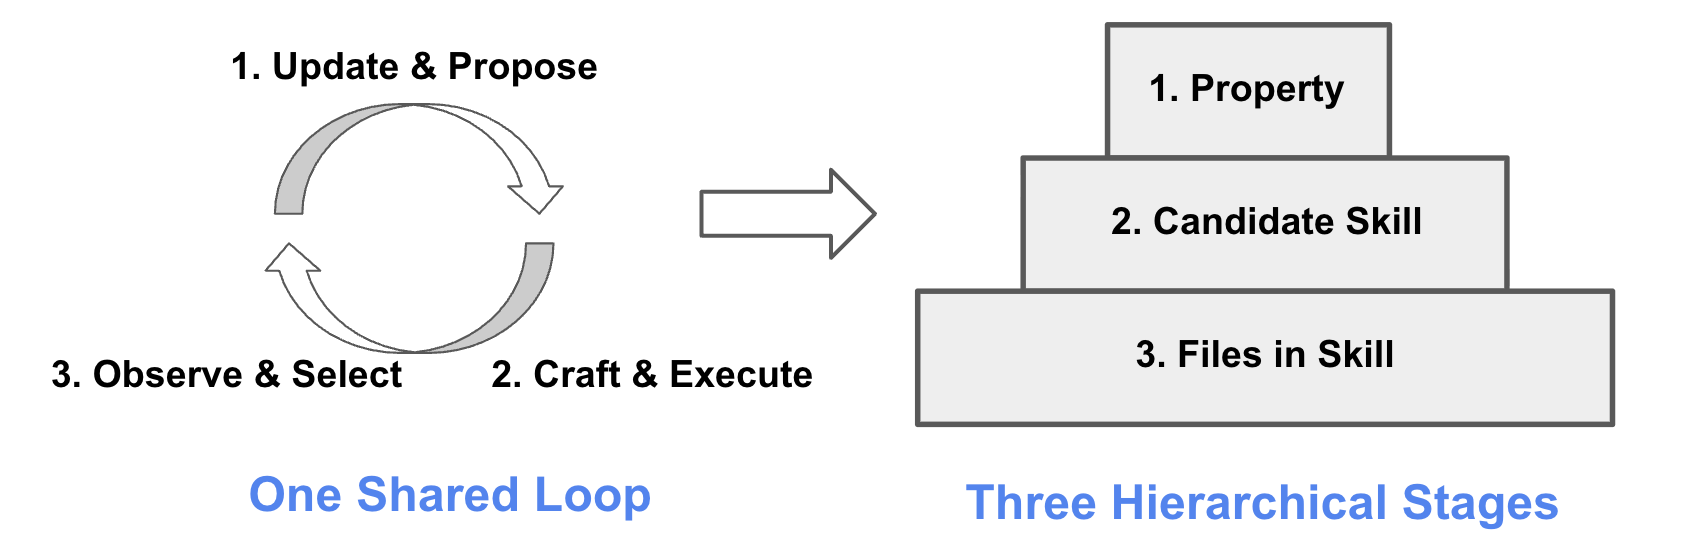
\includegraphics
    [width=\columnwidth]
    {DayDreaming.png}
    \vspace{-20pt}
    \caption{Architecture of \method}
    \label{fig:method-pipeline}
\end{figure}

Every experiment records its crafted task, observed result, decision, and supporting evidence in $\mathcal{O}$. 
Figure~\ref{fig:method-pipeline} summarizes the three-stage architecture and shared refinement loop, while 
Algorithm~\ref{alg:dd} gives the full pipeline. All victim calls share the fixed budget $B$, with remaining parameters listed in Table~\ref{tab:daydreaming-defaults}. Appendix~\ref{app:algorithm} provides complete pseudocode, Appendix~\ref{app:prompts} gives the default prompts, and our implementation is available online.\footnote{Source code: \url{https://github.com/anonymous/REPOSITORY}.}

% Every experiment adds its crafted task, result, decision, and
% supporting evidence to log $\mathcal{O}$.  Figure~\ref{fig:method-pipeline} shows
% both structures: progress across the three stages and the loop repeated within
% each stage. Algorithm~\ref{alg:dd} offers the overall pipeline of \method.  All victim calls share the fixed
% budget $B$, and remaining parameters appear in Table~\ref{tab:hyperparameters}. 
% We next explain each stage step by step and how each stage adapts to the three-phase loop structure mentioned above.  
% Appendix~\ref{app:algorithm} gives complete pseudocode, Appendix~\ref{app:prompts} gives the default prompts, and
% our implementation is available online.\footnote{Source code:
% \url{https://github.com/anonymous/REPOSITORY}.}


% \begin{figure*}[t]
%   \centering
%   \begingroup
%   \tcbset{stagecard/.style={colback=white, colframe=black!45,
%     boxrule=0.45pt, arc=1.5mm, boxsep=0pt,
%     left=5pt, right=5pt, top=4pt, bottom=3pt,
%     before skip=0pt, after skip=0pt, height=26mm, valign=top}}
%   \begin{tcolorbox}[enhanced, colback=black!1, colframe=black!25,
%     boxrule=0.4pt, arc=3mm, boxsep=0pt,
%     left=5pt, right=5pt, top=3pt, bottom=3pt,
%     drop shadow={black!35, opacity=0.35}]
%   \centering
%   {\sffamily\bfseries\scriptsize SAME LOOP IN EVERY STAGE:}\\[-1pt]
%   {\scriptsize \textbf{1} Update and Propose
%     $\rightarrow$ \textbf{2} Craft and Execute
%     $\rightarrow$ \textbf{3} Observe and Select
%     $\circlearrowleft$ next experiment}\\[4pt]

%   \begin{tabularx}{\linewidth}{@{}X@{\hspace{5pt}$\Longrightarrow$\hspace{5pt}}X@{\hspace{5pt}$\Longrightarrow$\hspace{5pt}}X@{}}
%     \begin{tcolorbox}[stagecard]
%       {\sffamily\bfseries\scriptsize STAGE 1 $\cdot$ PROPERTY}\\[3pt]
%       {\scriptsize \textbf{1}\enspace Severity vs. time}\\[1pt]
%       {\scriptsize \textbf{2}\enspace Task: low first, high later}\\[1pt]
%       {\scriptsize \textbf{3}\enspace Select severity ordering}\\[3pt]
%       {\color{black!55}\scriptsize Generalist shadow supplies context.}
%     \end{tcolorbox}
%     &
%     \begin{tcolorbox}[stagecard]
%       {\sffamily\bfseries\scriptsize STAGE 2 $\cdot$ CANDIDATE SKILL PLAN}\\[3pt]
%       {\scriptsize \textbf{1}\enspace Merge vs. repeat hits}\\[1pt]
%       {\scriptsize \textbf{2}\enspace Task: same indicator twice}\\[1pt]
%       {\scriptsize \textbf{3}\enspace Revised winner advances}\\[3pt]
%       {\color{black!55}\scriptsize Two candidate shadows predict results.}
%     \end{tcolorbox}
%     &
%     \begin{tcolorbox}[stagecard]
%       {\sffamily\bfseries\scriptsize STAGE 3 $\cdot$ FILE VERSION}\\[3pt]
%       {\scriptsize \textbf{1}\enspace Strict vs. inclusive cutoff}\\[1pt]
%       {\scriptsize \textbf{2}\enspace Task: alert at the cutoff}\\[1pt]
%       {\scriptsize \textbf{3}\enspace Select and revise the file}\\[3pt]
%       {\color{black!55}\scriptsize Reuse prior results and local tests.}
%     \end{tcolorbox}
%   \end{tabularx}

%   \vspace{3pt}
%   {\scriptsize Only the crafted task goes to the victim; proposals, shadows,
%   tests, and selections remain attacker-side.}
%   \end{tcolorbox}
%   \endgroup
%   \caption{Each stage applies the same three-step loop to a more concrete
%   choice.  The alert-triage example shows how each stage specializes the task
%   and comparison.  Stage~2 advances revised winners through adjacent-pair
%   rounds; Stage~3 reuses earlier results and crafts at most one new logical task
%   per file.}
%   \label{fig:method-pipeline}
% \end{figure*}

\subsection{Stage 1: Property Inference}
\label{sec:Stage~1}

% \paragraphtitle{Goal and outputs}
% Stage~1 learns individual behaviors before deciding how to organize them into a
% skill.  It starts from the public card $d$, the service's accepted task format,
% threat level $\ell$, and budget $B_1$.  It produces $P$, a set of tested
% property records; $\mathcal{O}$, the crafted tasks and victim results behind
% them; and $A$, helper filenames found in those results.  Each record in $P$
% contains the property tested, its alternatives, the selected outcome, and the
% supporting evidence.  Stage~2 uses $P$ and $A$; $\mathcal{O}$ is kept for
% Stage~3 and final assembly.

\paragraphtitle{Goal and outputs}
Stage 1 learns individual behavioral properties of the hidden skill before deciding how those properties are organized into a complete skill. It starts from the public card $d$, the service’s accepted task format, threat level $\ell$, and budget $B_1$. It produces $P$, a set of tested property records; $\mathcal{O}$, the crafted tasks and victim results behind them; and $A$, helper filenames observed in those results. Each record in $P$ contains the tested property, its alternatives, the selected outcome, and the supporting evidence. Stage 2 uses $P$ and $A$ to construct candidate skill plans, while $\mathcal{O}$ is retained for later stages and final assembly.

\paragraphtitle{1. Update and Propose}
The attacker model begins with $n_{\mathrm{seed}}$ possible properties suggested by the public card $d$. The prompt covers possible capabilities, constraints, procedures, terminology, input/output formats, decision rules, and supporting files (see Appendix~\ref{app:prompts}). For each property $c$, it proposes $n_{\mathrm{alt}}$ realistic alternatives $\mathcal{C}(c)$. New victim results may revise an existing property or suggest a follow-up property, so later experiments depend on what Stage~1 has already learned.

\paragraphtitle{2. Craft and Execute}
Stage~1 crafts tasks in three ways, all following the same rule: the proposed alternatives must predict visibly different task results. If no task can separate the alternatives, \method makes no victim call.

\begin{itemize}
    \item \emph{Ordinary behavior.}
    For properties such as result ordering, output format, or decision behavior, Stage~1 chooses inputs that make the alternatives produce different visible results. Properties that fit naturally in one task may be tested together. The victim then performs the crafted task.

    \item \emph{Numeric cutoffs.}
    When a tested property suggests a cutoff, Stage~1 creates an ordered batch of routine cases spanning a plausible range while keeping other inputs fixed. The task asks for one decision per case. If the decisions change consistently, a later adaptive task may test a narrower range around that change.

    \item \emph{Counting rules.}
    When an operation has several reasonable counting rules, Stage~1 creates a small input for which the alternatives predict different exact totals. For example, in \textit{alert-triage}, one DNS packet may count only as DNS, as DNS and UDP, or as DNS, UDP, and IP. The task asks the victim for the corresponding totals.
\end{itemize}

After each victim task, the generalist shadow performs the same task without a skill. Stage~1 uses this comparison to determine whether the observed behavior appears specific to the hidden skill or can already be reproduced by a generalist agent. The victim result remains the source of the selected property value.

\paragraphtitle{3. Observe and Select}
\method uses the strongest evidence available under threat level $\ell$: at Differential ($o_1$), it can additionally compare against the matched unskilled execution; at Trace ($o_2$), it observes the victim’s client-visible tool activity; and at Output ($o_3$), it relies only on the final message and returned files.
% \method uses the strongest evidence available under threat level $\ell$: visible execution records when available ($o_1$), locally runnable returned files when present ($o_2$), and returned text otherwise ($o_2$). 
For ordinary behavior, it records an alternative as \emph{confirmed} when the result follows it, \emph{refuted} when the result follows another alternative, and \emph{undetermined} otherwise. For a cutoff, it requires the decisions to change once in a consistent direction; if the returned material exposes the exact comparison, that value replaces the estimate. For a counting rule, it selects the unique rule whose predicted totals exactly match the victim result. No cutoff or counting rule is selected when the result is incomplete or inconsistent.

% \method reads the strongest evidence available: a visible execution record
% first, a locally runnable returned file when available, and returned text as a
% fallback.  For ordinary behavior, it records an alternative as
% \emph{confirmed} when the result follows it, \emph{refuted} when the result
% follows another alternative, and \emph{undetermined} otherwise.  For a cutoff,
% it requires the decisions to change once in a consistent direction; if the
% returned material exposes the exact comparison, that value replaces the
% estimate.  For a counting rule, it selects the unique rule whose predicted
% totals exactly match the victim result.  No cutoff or counting rule is selected
% when the result is incomplete or inconsistent.

Stage~1 also extracts additional evidence from already collected results at no extra victim cost. It scans stored code and task results for module names, function names, calls, commands, and paths that were not supplied by the crafted task. 
% For example, \texttt{port\_entropy(flows)} reveals both a visible function name and its expected input shape. 
Filenames found in victim results are added to $A$ only after removing names copied from the crafted task and obvious task-output files.

% At no extra victim cost, Stage~1 also reads stored code and task results for
% module names, function names, calls, commands, and paths that were not supplied
% by the crafted task.  For instance, \texttt{port\_entropy(flows)} reveals a
% visible function name and its input shape.

Before a record enters $P$, its wording is restricted to details supported by the victim result. A failed or undetermined test containing only the attacker’s guess is dropped. Stage~1 adds each crafted task, victim result, decision, and supporting evidence to $\mathcal{O}$.

% Before a record enters $P$, its wording is restricted to details present in the
% victim result.  A failed or undetermined test containing only the attacker's
% guess is dropped.  Stage~1 adds the crafted task, result, decision, and evidence
% to $\mathcal{O}$.  It adds to $A$ only filenames found in victim results after
% removing names copied from the task and obvious task output files.

\paragraphtitle{Running example}
\emph{Update and Propose:} Stage 1 proposes that security findings are ordered either \textit{by severity} or \textit{by detection time}. \emph{Craft and Execute:} it creates a report task in which a low-severity event occurs first and a high-severity event occurs later, so the two alternatives predict opposite row orders. \emph{Observe and Select:} if the victim places the high-severity row first, Stage~1 records severity ordering and the returned row order as supporting evidence. A later loop can apply the same process to an escalation cutoff: propose a plausible range, submit a batch of alerts spanning that range, and narrow the cutoff based on where the victim’s decisions change.

% \emph{Update and Propose:} Stage~1 proposes that security findings are ordered either \textit{by severity} or \textit{by detection time}.  
% \emph{Craft and Execute:} it creates a report
% task in which a low-severity event occurs first and a high-severity event occurs
% later, so the alternatives predict opposite row orders.  \emph{Observe and
% Select:} if the victim places the high-severity row first, Stage~1 records
% severity ordering and the returned row order as evidence.  A later loop can reuse
% the same pattern for an escalation cutoff: propose a range, send a batch
% of alerts across it, and record where the victim's decisions change.

\subsection{Stage 2: Candidate Selection}
\label{sec:stage2}

\paragraphtitle{Goal and limitation}
Stage~1 identifies behavioral properties of $S$ but does not determine how those properties are organized into a multi-file skill. The same observed behavior may come from instructions, a script, or a reference file. Stage~2 therefore compares complete \emph{candidate skill plans} rather than isolated properties. It returns a plan $H^\star$ that is consistent with the observed behavior, but not necessarily with the vendor’s original file organization.

\paragraphtitle{1. Update and Propose}
Let $H_i=(m_i,\mathcal{R}_i)$ denote a candidate skill plan, where $m_i$ is a draft \texttt{SKILL.md} and each entry in $\mathcal{R}_i$ specifies a supporting file’s path, purpose, and content sketch. Stage~2 constructs a set $\mathcal{H}={H_1,\ldots,H_{n_H}}$ of candidate plans. Every plan must preserve the tested properties in $P$ and include filenames observed in $A$, while making different choices where the evidence remains incomplete.

To encourage diverse but plausible structures, the attacker model proposes $n_H$ representative customer tasks, each pairing a user role with a concrete use of the skill, and drafts one candidate plan around each task (see Appendix~\ref{app:prompts}). A plan may also propose supporting files beyond $A$, since Stage~1 may not expose every file used by the hidden skill.

Stage~2 compares plans in pairs across rounds. The selected plan is revised with newly supported behavior and advances to the next round, while an unpaired plan receives a bye. Thus, later rounds use both the original evidence in $P$ and $A$ and the victim results accumulated during earlier comparisons.


% Let $H_i=(m_i,\mathcal{R}_i)$ denote one candidate skill plan.  Here, $m_i$ is a
% draft \texttt{SKILL.md}; each entry in $\mathcal{R}_i$ gives a supporting
% file's path, purpose, and content sketch.  
% Stage~2 creates a set of $\mathcal{H}=\{H_1,\ldots,H_{n_H}\}$ candidate skill plans.
% Every plan follows the tested properties in $P$ and includes the filenames in
% $A$.  These records describe observed behavior, but they may not show how the
% behaviors interact or how the skill divides them across files.  The attacker
% model therefore proposes $n_H$ representative customer tasks, each pairing a
% user role with a concrete use of the skill, and drafts one candidate plan for
% each task while encouraging different plans (see system prompts in Appendix~\ref{app:prompts}).  
% A plan may also propose supporting files beyond $A$, because Stage~1 may not
% expose every file used by the skill.

% Stage~2 compares adjacent pairs in each round.  The chosen plan is revised with
% newly supported behavior and advances to the next round; an unpaired plan
% receives a bye.  Thus, Update and Propose uses both the original records $P$
% and results accumulated in earlier rounds.

\paragraphtitle{2. Craft and Execute}
For a pair of plans $(H_a,H_b)$, the attacker model uses the Stage~2 comparison
prompts to construct $D(H_a,H_b)$, the behavioral differences that would change
a task result (Appendix~\ref{app:prompts}).  Differences only in filenames or
file placement are excluded since any crafted task cannot distinguish them.
If $D(H_a,H_b)$ is empty, \method makes no victim call.  Otherwise, it crafts
a task $x_{a,b}$ that exposes one or more of these differences and sends only
that task to the victim. 
The attacker model also performs $x_{a,b}$ through candidate shadows for
each plan.  A candidate shadow receives $H_a$ or $H_b$ and the task $x_{a,b}$, and produces the
result predicted by that plan.  Let $y_v$ be the victim result and $y_a,y_b$ be
the two candidate-shadow results.  Stage~2 compares these three results while
retaining richer victim observations in $\mathcal{O}$.

\paragraphtitle{3. Observe and Select}
For each difference in $D(H_a,H_b)$, Stage~2 checks whether $y_v$ follows
$y_a$, $y_b$, both, or neither.  The plan matching more differences becomes the survivor.  
Stage~2 then revises it with behavior supported by the victim result, including any point on which the
other plan matched better, while preserving the measured properties and
observed filenames required by $P$ and $A$.  It stores the crafted task, the
three results, the decision, and the revised survivor in $\mathcal{O}$.

A tie, a result matching neither plan, or the absence of a
discriminating task does not identify either plan.  Since Stage~2 must
produce one plan for Stage~3, it uses an explicit fallback:
prefer greater coverage of $A$, then fewer files, then the earlier plan.  This
fallback keeps the three-phase loop moving.  With $n_H$ initial plans, Stage~2 performs at
most $n_H-1$ pairwise comparisons.  Its output $H^\star$ is the final revised
survivor.

\paragraphtitle{Running example}
\emph{Update and Propose:} both plans preserve the alert cutoff recovered in
Stage~1, but $H_a$ merges repeated indicator hits while $H_b$ reports every hit.
\emph{Craft and Execute:} Stage~2 creates an alert containing the same indicator
twice; the victim performs it, and the two candidate shadows predict one versus
two findings.  \emph{Observe and Select:} if the victim returns one finding,
$H_a$ survives and is updated before its next round.  If the plans differed
only in whether that rule appears in \texttt{SKILL.md} or a script, no task
would distinguish them and the layout choice would use the stated fallback.

\subsection{Stage 3: Per-File Refinement}
\label{sec:stage3}

\paragraphtitle{Goal and outputs}
Stage 2 returns one candidate skill plan $H^\star=(m^\star,\mathcal{R}^\star)$, where $m^\star$ is the draft instruction file and each entry in $\mathcal{R}^\star$ specifies only the path, purpose, and content sketch of a supporting file. Stage~3 keeps this file structure fixed and turns each sketch into complete file content. It processes supporting files first and the instruction file last, so the final instructions can refer to the actual function names, interfaces, and paths in the completed files. The output is the final reconstruction $\widehat{S}=(\widehat{m},\widehat{\mathcal{R}})$.

% \paragraphtitle{Input and goal}
% Stage~2 returns one candidate skill plan
% $H^\star=(m^\star,\mathcal{R}^\star)$.  Here, $m^\star$ is the draft instruction file, 
% while each entry in $\mathcal{R}^\star$ gives only the path,
% purpose, and content sketch of a supporting file.  Stage~3 keeps this file list
% fixed and turns every sketch into complete content.  It processes the supporting
% files first and instruction file last, so the final instructions can use the
% actual function names and inputs in the completed files.  The result is
% $\widehat{S}=(\widehat{m},\widehat{\mathcal{R}})$.

\paragraphtitle{1. Update and Propose}
For each supporting file $f\in\mathcal{R}^\star$, the attacker model first
expands its path, purpose, and sketch into one complete version.  It treats the
draft $m^\star$ as the initial instruction-file version and processes it last.
For each file, it then identifies uncertain choices---for
example, whether a cutoff uses $>$ or $\geq$---and proposes complete versions
that make different choices (see system prompts in Appendix~\ref{app:prompts}).
Let $V_f$ denote this set of complete versions.  After each comparison, the
selected version is revised at its weakest checked behavior and becomes the
starting point for the next round.

\paragraphtitle{2. Craft and Execute}
For one fixed file $f$, the attacker model constructs $D_f$,
representing the differences among versions in $V_f$ that would change a
task result (Appendix~\ref{app:prompts}).  If $D_f$ is empty, \method makes no
victim call.  Otherwise, it crafts a task $x_f$ that exposes one or more of
these differences and submits it to the victim.  An unusable first transmission
may be shortened and retried once, with both transmissions charged to $B_3$.
We denote the same task $x_f$; let $t_{f,v}$ denote the result produced while following
version $v \in V_f$. Stage~3 later compares these shadow results with the victim result
$t_f$.  Any additional execution details remain stored in $\mathcal{O}$.  

For instruction and reference files, Stage~3 also compares versions against
stored task-result pairs from Stages~1 and~2.  When an earlier result reflects
behavior governed by $f$, it provides another comparison for $V_f$ without a
new victim call.  Thus, Stage~3 obtains at most one new usable victim result per
file and reuses earlier results whenever they apply.

\paragraphtitle{3. Observe and Select}
For each version $v\in V_f$, Stage~3 checks whether $t_{f,v}$ matches $t_f$ on
the behaviors exposed by $D_f$.  For instruction and reference files, candidate
shadows also perform the stored tasks from Stages~1 and~2 and compare their
results with the stored victim results.

The version agreeing best with the observed behavior becomes the current
selected version.  The attacker model revises its weakest observed mismatch
and repeats the comparison attacker-side using the same results.  A revision is kept if its
average score improves, or if no current version scores higher on every checked
behavior; Algorithm~\ref{alg:dd-stage3} in the appendix gives the complete
rule.  Malformed files, wrappers that require an unavailable external copy,
and changes to recovered constants are rejected.  After refining every supporting file,
Stage~3 refines the instruction file last against their completed files.

If no crafted task distinguishes $V_f$, or no usable victim result is returned,
Stage~3 falls back to the stored results from Stages~1 and~2 for instruction or
reference files and to local tests for executable files.  If neither source
distinguishes the versions, it marks $f$ unresolved and keeps the initial
valid version.  This fallback permits the loop to continue.

\paragraphtitle{Running example}
\emph{Update and Propose:} for the detector script, Stage~3 creates complete
versions that differ only in whether the recovered cutoff uses $>$ or $\geq$.
\emph{Craft and Execute:} it sends the victim one alert exactly at the cutoff,
stores the verdict as $t_f$, and runs both versions and a local test
attacker-side.  \emph{Observe and Select:} it keeps the version matching $t_f$;
the local test rejects a script that states the right comparison but never
applies it.  Every later revision reuses the same result.

\subsection{Assembly}
\label{sec:assembly}

After Stage~3, \method writes the selected files to their planned relative
paths.  Stage~2 has already inserted the filenames in $A$, and Stage~3 has
verified that those paths remain present.  Assembly then performs two guarded
offline cleanups: replacing fixed spreadsheet ranges
and missing-value placeholders with general rules, and making absolute output
paths caller-chosen.  A rewrite is kept only if it removes the flagged detail
without dropping recovered interfaces or changing other paths; otherwise, the
original is retained.  These checks make no victim calls and cover only these
known patterns, so other task-specific details may remain.  The assembly steps
appear at the end of Algorithm~\ref{alg:dd-stage3}.

\begin{comment}
  \subsection{Access Levels}
  \label{sec:access-adapters}
  
  The three access levels expose nested observations
  $o_1(x)\supseteq o_2(x)\supseteq o_3(x)$.  The stage structure and the
  discriminating-task generator remain the same; the readout and strength of
  attribution change with $\ell$.  Because the attack is adaptive, different
  observations may still lead later end-to-end runs to choose different tasks.
  
  \paragraphtitle{Output ($\ell=3$), the primary setting.}
  The attacker sees the final reply and returned files.  It reads properties from
  that material and may execute returned code locally.  Its only general control
  is the attacker model performing the same task without a skill.  A disagreement
  is suggestive of skill-specific behavior, but not causal evidence: the two runs
  also differ in model, prompt, and sampling.
  
  \paragraphtitle{Trace ($\ell=2$).}
  The observation additionally includes client-visible tool calls and their
  results.  A trace-based readout takes precedence over local re-execution and
  text because it records what the victim actually ran in its own environment.
  The attacker-side control is projected through the same kind of readout before
  branches are compared, avoiding an execution-versus-text mismatch.  The base
  model and hidden skill are still not isolated, so attribution remains
  correlational.
  
  \paragraphtitle{Differential ($\ell=1$).}
  The attacker knows the deployment well enough to run a matched unskilled twin
  $\mathcal{V}_{\varnothing}$ on the same task.  The twin shares the base model,
  harness, tools, decoding settings, and customer persona; the installed skill is
  the intended difference.  A branch taken by $\mathcal{V}_S$ but not by
  $\mathcal{V}_{\varnothing}$ is therefore stronger evidence that the skill caused
  the behavior.  This conclusion depends on the match being exact and on the
  paired calls succeeding, so the observation log records ``no control'' separately from
  ``control agreed.''
  
\end{comment}

\section{Evaluation}

\label{sec:evaluation}

We evaluate \method through three research questions:

\noindent\textbf{RQ1: Performance.}
We evaluate the performance of \method concerning three major factors below:
\begin{itemize}
    \item How much utility does \method recover from the strictest Output($o_3$) threat level, relative to no-skill and original skill setting as well as prior attacks and baselines?
    \item How much structural recovery can \method achieve relative to the original skill?
    \item How does each component throughout different stage contribute to \method, and how does utility of \method change with varying attacker query budget?
\end{itemize}
\noindent\textbf{RQ2: Observability.}
How does \method performs when the victim deploys skill across different threat levels $o_1$, $o_2$, and $o_3$? 

\noindent\textbf{RQ3: Transferability.}
Once \method successfully reconstruct skill $\hat{S}$, does it remain useful across victim models and orchestration/tool policy?

\subsection{Experimental Settings}
\label{sec:experimental-settings}

\paragraphtitle{Dataset}
Adapted from SkillsBench~\cite{skillsbench}, we select 7 skills as the stealing target with details summarized in Table~\ref{tab:factor-results}. 
We select the skills based on the criterion of real-world use cases, spanning use case such as rule/table lookup, numeric algorithms, procedures/checklists, workflow orchestration, and document/artifact production, we also add the criterion that installing the original skill must improve task performance over the no-skill condition.

Furthermore, following the objective defined in Section~\ref{sec:access-levels}, we construct a held-out dataset $\mathcal{B}$ of 5 tasks curated from SkillsBench~\cite{skillsbench}. Each task in the has its own input $x$ and its executable verifier $v_x$. Due to the design of SkillsBench~\cite{skillsbench}. Each task requires one or multiple skills to cooperate to complete the task. For instance, a task such as \textit{network intrusion} requires skills such as \textit{pcap-analysis} and \textit{threat-detection}. Since each task may depend on several skills, so we treat is as the basic unit in reporting the metrics.

\begin{table}[t]
  \centering
  \caption{Task-to-skill mapping for the evaluation dataset.}
  \label{tab:benchmark-map}
  \scriptsize
  \setlength{\tabcolsep}{4pt}
  \renewcommand{\arraystretch}{1.08}
  \begin{tabularx}{\columnwidth}{@{}
    >{\raggedright\arraybackslash}p{0.40\columnwidth}
    >{\raggedright\arraybackslash}X
  @{}}
    \toprule
    \textbf{Task} & \textbf{Required skill package(s)} \\
    \midrule
    \texttt{protein-expression-analysis}
      & \texttt{xlsx} \\
    \addlinespace[2pt]

    \texttt{pddl-airport-planning}
      & \texttt{pddl-skills} \\
    \addlinespace[2pt]

    \texttt{pddl-tpp-planning}
      & \texttt{pddl-skills} \\
    \addlinespace[2pt]

    \texttt{dapt-intrusion-detection}
      & \texttt{pcap-analysis}, \texttt{threat-detection} \\
    \addlinespace[2pt]

    \texttt{software-dependency-audit}
      & \texttt{cvss-score-extraction},
        \texttt{trivy-offline-vulnerability-scanning},
        \texttt{vulnerability-csv-reporting} \\
    \bottomrule
  \end{tabularx}
\end{table}

Each task in the dataset is fully held out, including prompts, inputs, and verifier are never used as victim queries, shadow-agent tasks, local tests, or candidate-selection signals. Table~\ref{tab:benchmark-map} also makes clear the task-skill mapping.

\paragraphtitle{Model Setting}
For victim model selections, we opt for both closed-weight and open-weight models which are \texttt{claude-opus-5}, \texttt{gpt-5.6-sol}, and \texttt{kimi-k3}. Moreover, we selected \texttt{claude-opus-5} as the default victim if not further announced. We select \texttt{gemini-3.7-flash} as the attacker model across evaluations. All victim uses temperature 0.2 and top-$p=0.95$, whereas the attacker uses temperature 0.7 and top-$p=0.95$.  For each reconstructed skill, we evaluate the held-out dataset on \texttt{glm-5.3} as the default deployment for evaluation. RQ3 further tests the transferability of these recovered skills across all victim models. 

\paragraphtitle{Orchestration / Tool Policy Setting}
We select \texttt{deepagents} as the default policy setting, which are constructed with filesystem and several basic tools. For additional policy settings, we also include \texttt{claude\_agent\_sdk}, \texttt{openai\_agents}, and \texttt{agno} with details in Appendix~\ref{app:evaluation-details}. 

%the \texttt{ls}, \texttt{read\_file}, \texttt{write\_file},
%\texttt{edit\_file}, \texttt{glob}, \texttt{grep}, \texttt{delete},
%\texttt{execute}, and \texttt{task} 

\paragraphtitle{Threat Level Setting}
Consistent with our threat model, the attacker receives the public skill card but not the skill $S$, held-out tasks, verifiers, or victim memory and reasoning process. We use the observation names defined by the threat model: \emph{Output} reveals returned text and files, \emph{Trace} additionally
reveals task-level tool events, and \emph{Differential} adds the model and
harness stack plus a matched no-skill execution. This allows the attack to adapt only to the view it receives. 

\paragraphtitle{Daydreaming Setting}
The default per-skill budget is $B=96$, divided into 64 stage~1, 12 stage~2, and 20 stage~3 calls. The attack seeds 14--18 properties, groups at most four per probe, generates six package hypotheses, creates up to three initial version per file. Differential unskilled twin calls are recorded separately from victim budget calls.  The complete parameter list is
in Appendix~\ref{app:evaluation-details}.

\paragraphtitle{Prior Attacks and Baseline Setting}
For a fair, resource-aligned comparison, BBS and SigLeak use the same three victims, \geminimodel{} attacker, and budget as \method, while retaining its native probing and stopping rule rather than being forced to spend identical calls. Its native input is a signed augmented trajectory; we therefore label it \emph{augmented trace} and do not claim Output-threat level compatibility. Costs are reported for producing a complete reconstructed skill in each method's native form. 

Furthermore, we evaluate two additional baseline that accompanied this setting, which are called \textit{Fixed Probes} and \textit{One-pass synthesis} which we describe below. For \textit{One-pass synthesis}, the attacker model is only given the public card $d$ and asked to generate the reconstructed skill with one pass only and no other queries are allowed. \textit{Fixed Probes} is a more informative baseline than \textit{One-pass Synthesis} as the attacker model are able to craft all tasks in advance and received its results. Then along with the public skill card, it is asked to generate the reconstructed skill $\widehat{S}$.  

\begin{figure*}
    \centering    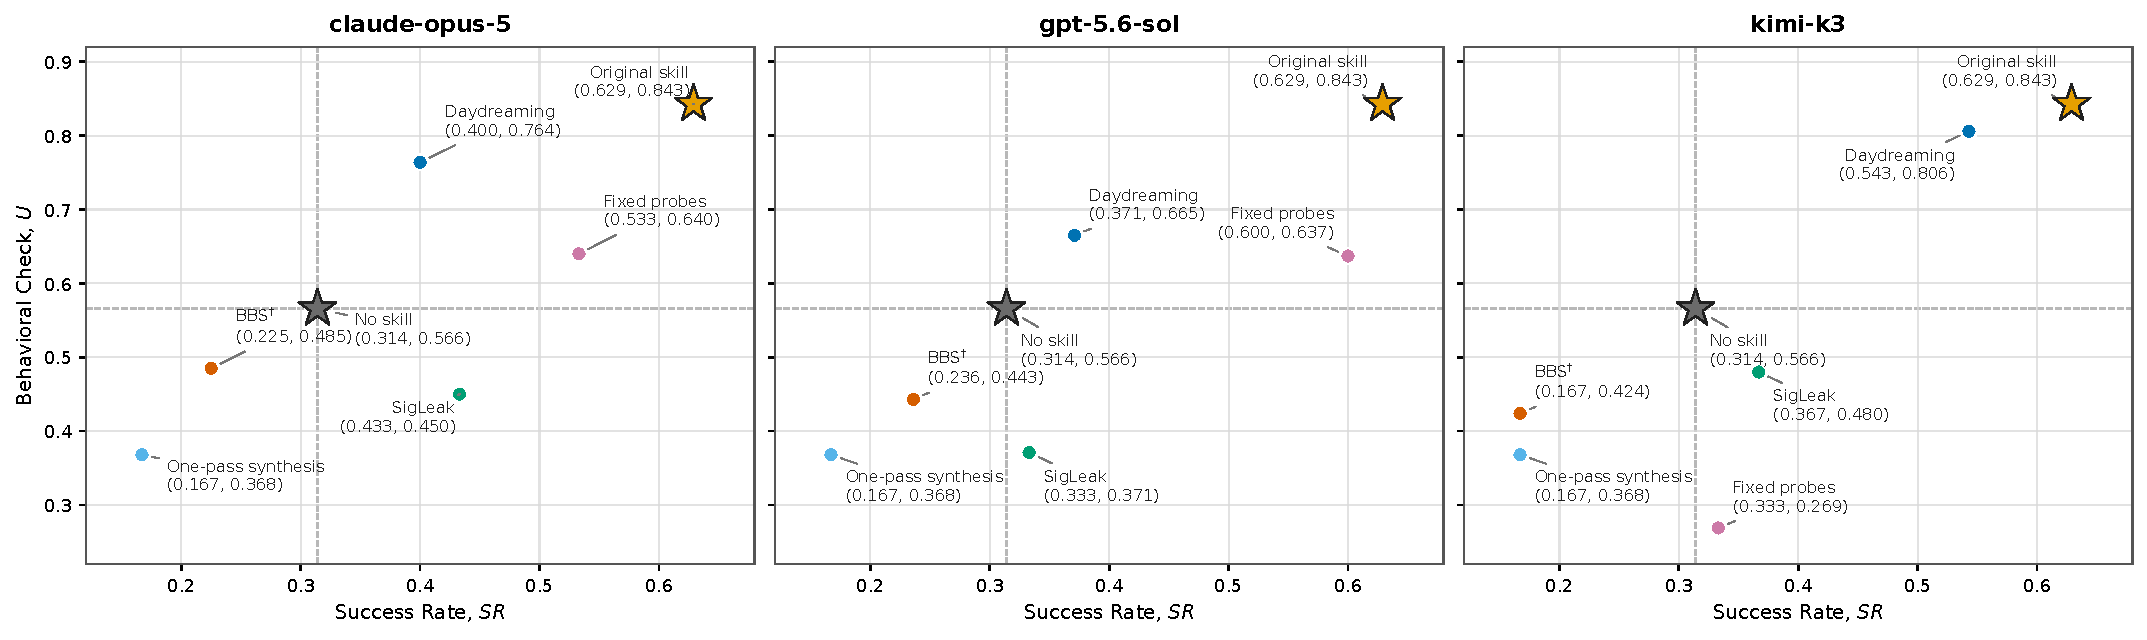
\includegraphics[width=\textwidth,keepaspectratio]{figures/T03.pdf}
    \caption{Comparison with prior attacks and baselines.}
    \label{fig:baseline-results}
\end{figure*}
\subsubsection{Metric.}
Let $C$ denote the installed package condition: no skill $\emptyset$, a
reconstruction skill $\widehat{S}$, or the original skill $S$.
For task $b$, due to the stochastic nature of the victim model $M$ along with the policy $\Pi$, we run in total $n_b$ trials to solicit the final results. For each trial with index $i$, it has a final verifier  binary result $y_{bi}(C)\in\{0,1\}$. As a result, we define the first metric of binary success as
\[
 \operatorname{SR}_b(C)=\frac{1}{n_b}
   \sum_{i=1}^{n_b} y_{bi}(C)
\]
$SR$ denotes strict binary success, meaning the end-to-end completion of task $b$.

On the other hand, we grade the skill's utility also with a trace-related metric, which capture the agent's correct behaviors in trace rather than final success. Specifically, given trial $i$, task $b$ and condition $c$, the task offers in total $m_{bi}(C)$ intermediate verifier checks while the agent might pass $p_{bi}(C)$ of them. We define the second metric of behavior check as
\[
 U_b(C)=\frac{\sum_i p_{bi}(C)}{\sum_i m_{bi}(C)}.
\]
$U$ denotes behavioral utility. This is the empirical instantiation of $U(P)$ defined in Section~\ref{}. Since a task might span multiple skills, we report the overall task average as 
\[
 \operatorname{SR}(C)=\frac{1}{|\mathcal{B}|}\sum_{b\in\mathcal{B}}
 \operatorname{SR}_b(C),\qquad
 U(C)=\frac{1}{|\mathcal{B}|}\sum_{b\in\mathcal{B}}U_b(C),
\]

We further define normalized binary and behavioral success recovery across tasks as
\[
 \operatorname{NSR}(C)=
 \frac{\operatorname{SR}(C)-\operatorname{SR}(\emptyset)}
      {\operatorname{SR}(S)-\operatorname{SR}(\emptyset)}, \qquad
 \mathrm{NU}(C)=
  \frac{U(C)-U(\emptyset)}
       {U(S)-U(\emptyset)}
\]
which denote the improvement ratio compared to original skill $S$. We note that 0 corresponds to no skill, 1 to the original skill, negative values indicate utility below no skill, and values above 1 indicate utility above the original skill.

We also report cost, elapsed time, and structural precision, recall, and F1. To compute the structural metrics, we match recovered numeric constants, threshold branches, tool preconditions and output schemas, file paths, and executable scripts one-to-one against their counterparts in the original version of the same skill, and then pool the counts across skills.

\subsection{Experimental Results}
\label{sec:experimental-results}

We organize the results by the three RQs.  All scores use the held-out tasks and metrics defined in Section~\ref{sec:experimental-settings}. 

\paragraphtitle{RQ1: Performance}\\
\emph{End-to-End utility.}
\begin{table*}[hbt]
  \centering
  \scriptsize
  \caption{Output-level results on held-out tasks. Task cells show
  $\mathrm{SR}_b/U_b$; summary rows show $SR$/$U$ and $NSR$/$NU$.}
  \label{tab:overall-results}
  \setlength{\tabcolsep}{5pt}
  \renewcommand{\arraystretch}{1.03}

  \begin{tabularx}{\textwidth}{@{}Yccccc@{}}
    \toprule
    Task ($\mathrm{SR}_b/U_b$)
      & No skill & \opusmodel & \solmodel & \kimimodel & Original \\
    \midrule
    Protein expression
      & .571/.786 & 1.000/1.000 & .857/.929 & 1.000/1.000 & .714/.857 \\
    Airport planning
      & .000/.357 & .143/.500 & .286/.571 & .000/.500 & .286/.571 \\
    Purchaser planning
      & 1.000/1.000 & .857/.857 & .571/.643 & 1.000/1.000 & 1.000/1.000 \\
    Network intrusion
      & .000/.153 & .000/.714 & .000/.398 & .000/.602 & 1.000/1.000 \\
    Dependency audit
      & .000/.536 & .000/.750 & .143/.786 & .714/.929 & .143/.786 \\
    \midrule
    \textbf{SR/U (task avg.)}
      & \textbf{.314/.566}
      & \textbf{.400/.764}
      & \textbf{.371/.665}
      & \textbf{.543/.806}
      & \textbf{.629/.843} \\
    \textbf{NSR/NU}
      & \textbf{.000/.000}
      & \textbf{.273/.716}
      & \textbf{.182/.358}
      & \textbf{.727/.868}
      & \textbf{1.000/1.000} \\
    \bottomrule
  \end{tabularx}
\end{table*}
Table~\ref{tab:overall-results} first compares \method with the no-skill and
original conditions under the Output($o_3$) threat level. Among the
reconstructions, \kimimodel{} is strongest, improving $SR$ from .314 to .543
and $U$ from .566 to .806. The \opusmodel{} reconstruction also improves both
metrics, reaching .400/.764. The \solmodel{} reconstruction reaches .371/.665
and remains above no skill on both metrics. Reconstruction quality therefore
depends on the source victim.

\noindent\emph{Comparison with prior attacks and baselines.}
Figure~\ref{fig:baseline-results} compares \method with prior attacks and baseline methods across three victim models, we delegate the exact experimental numbers to Appendix~\ref{app:evaluation-details}. The x-axis reports success rate (SR), while the y-axis reports the behavioral check score (U), with the upper-right corner indicating stronger overall performance. Across all three victims, \method consistently achieves the highest behavioral check score among all attack methods while approaching the performance of the original skill. Although Fixed Probes attains a higher SR on \opusmodel{} and \solmodel{}, it exhibits noticeably lower behavioral check scores, demonstrating that maximizing SR alone does not necessarily produce more useful or faithful behaviors. On \kimimodel{}, \method dominates prior attacks on both SR and behavioral check, illustrating a favorable balance between effectiveness and behavioral quality across different victim models.

\begin{table}[t]
  \centering
  \scriptsize
  \caption{Structural recovery for the \opusmodel.  P, R, and
  F1 denote precision, recall, and F1 score for recovery score.}
  \label{tab:granularity-results}
  \setlength{\tabcolsep}{2.5pt}
  \begin{tabularx}{\columnwidth}{@{}Yrrrr@{}}
    \toprule
    Item type & Total Counts & P & R & F1 \\
    \midrule
    Exact constants & 104 & .111 & .010 & .018 \\
    Threshold branches & 31 & .111 & .032 & .050 \\
    Tool preconditions/schemas & 19 & .000 & .000 & .000\\
    File paths & 7 & .333 & .143 & .200 \\
    Executable scripts & 2 & .125 & .500 & .200 \\
    Constants (within 1\% tolerance) & 104 & .556 & .048 & .088 \\
    \bottomrule
  \end{tabularx}
\end{table}



\noindent\emph{Structural recovery.}
Table~\ref{tab:granularity-results} further compares reconstructed structures with the original skills. Structural recovery is limited as constants and threshold branches obtain .018 and .050 F1, while paths and scripts reach .200. Combining with the previous experiments on end-to-end utility, we thus note that useful behavior does not require an exact copy to work.

\noindent\emph{Components and query budget.} Before we move into the results, we briefly recall each component used within stage and introduce them to better interpret the experimental results. 

For Stage~1 of \method, we ablate two essential component, which are the \textit{property labeling mechanism} (Observe\&Select) that attach each property $c \in P$ with an evidence label and the \textit{filename selecting protocol} (Observe\&Select) that uses victim task results to filter plausible filenames in $A$ . We ablated these two mechanism as they are the most fundamental part that constitute Stage~1's property-level identification.  

For Stage~2, we ablate two other components which are the \textit{number of candidate skill plan} (Update\&Propose) and the \textit{discriminating task generation} (Craft\&Execute). For the first one, we reduce the number of candidate skill plan in Stage~2 to $1$ meaning that once the attacker model came out with a skill plan $H$, we treat it as $H^*$ and proceed to Stage~3. For the second one, we ablate the discriminating task generation of Stage~2 and instead ask the attacker model to submit ordinary job pertaining to each candidate plan without considering their difference. As Stage~2 focus on more nuanced discrimination between each candidate skill, we chose these two mechanisms to ablate for.

Finally, for Stage~3, we ablate whether doing per-file refinement is useful for the utility of reconstructed skill.

Figure~\ref{fig:ablation-results} shows that every evaluated component contributes to the behavioral utility of the recovered skill. The largest utility drops occur when removing the Stage~1 filename-selection protocol and Stage~2 discriminating-task generation, which reduce $U$ to .624 and .626, respectively. Removing the Stage~1 property-label mechanism increases $SR$ from .400 to .497 but lowers $U$ to .696, which might be explainable due to the reason that verifying the property gives a stronger signal to the overall behavior but not the end effectiveness. Restricting Stage~2 to one candidate skill plan and removing Stage~3 per-file refinement leave $SR$ unchanged at .400, while reducing $U$ to .736 and .714, respectively. This indicate a even stronger signal that \method's later stage contributes mostly to the behavioral success of the reconstructed skill. Overall, every ablation lowers $U$, confirming that each component contributes to the quality of the reconstructed skill.

Table~\ref{tab:budget-results} studies sensitivity to the victim-call budget $B$. Among settings evaluated on all skills, behavioral utility increases from .762 at $B=32$ to .777 at $B=64$ and .785 at the default $B=96$, while SR varies non-monotonically and is highest at $B=32$. Thus, additional victim calls improve behavioral quality more consistently than raw task success, with diminishing gains at larger budgets. This demonstrated that larger call budget can recover behavioral success $U$ since each stage in \method are allowed more budget for fine-grained discrimination.

\begin{figure}[!t]
  \centering
  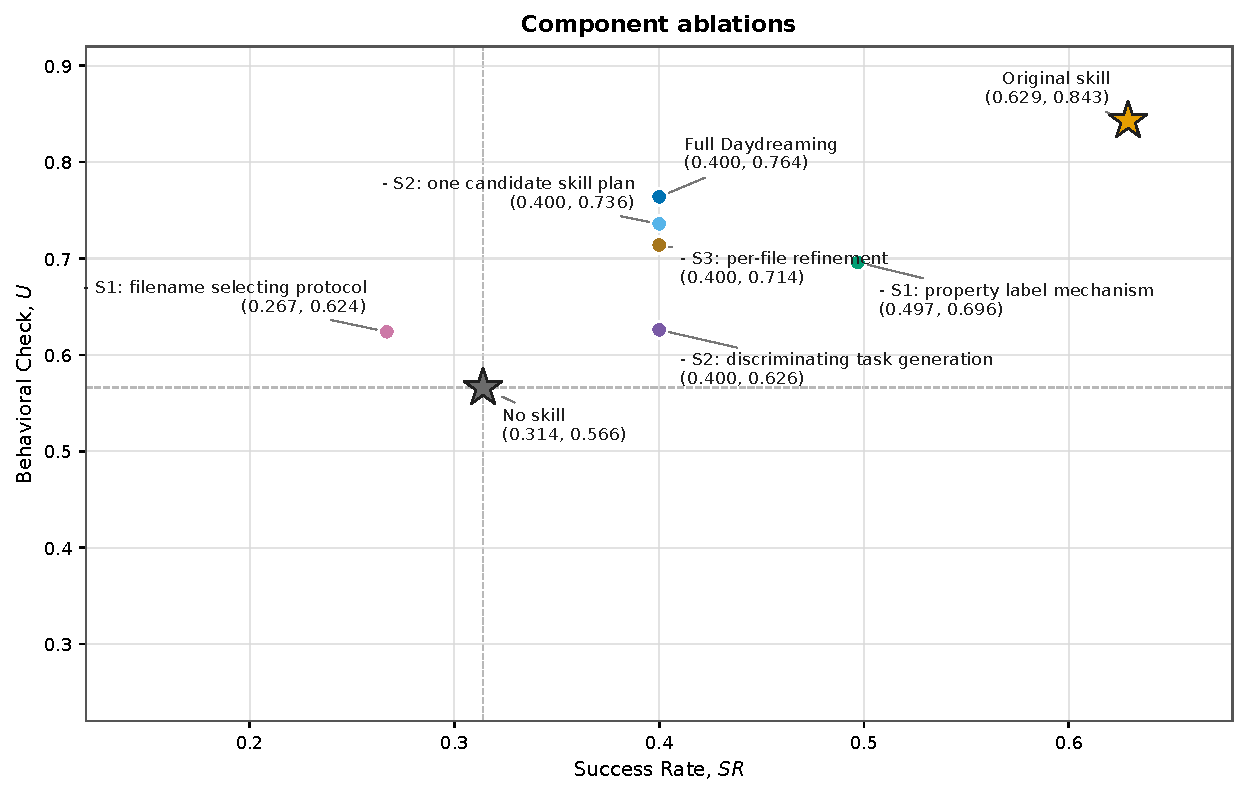
\includegraphics[width=\linewidth,keepaspectratio]{figures/T04.pdf}
  \caption{Component ablations.}
  \label{fig:ablation-results}
\end{figure}

\begin{table}[!t]
  \centering
  \scriptsize
  \caption{Victim-call budget sweep.}
  \label{tab:budget-results}
  \setlength{\tabcolsep}{2.8pt}
  \renewcommand{\arraystretch}{1.03}
  \begin{tabularx}{\columnwidth}{@{}Yrrr@{}}
    \toprule
    Victim Call Budget $B$  & $SR$/$U$ & Actual Queries per skill & cost per skill \\
    \midrule
    16  & .467/.740 & 15 & 7.07 \\
    32  & .433/.762 & 25.0 & 9.53  \\
    64  & .400/.764 & 29.6 & 12.31 \\
    96  & .476/.785 & 32.8 & 14.40 \\
    128 & .400/.788 & 29.3 & 12.94 \\
    \bottomrule
  \end{tabularx}
\end{table}


\begin{figure*}
\centering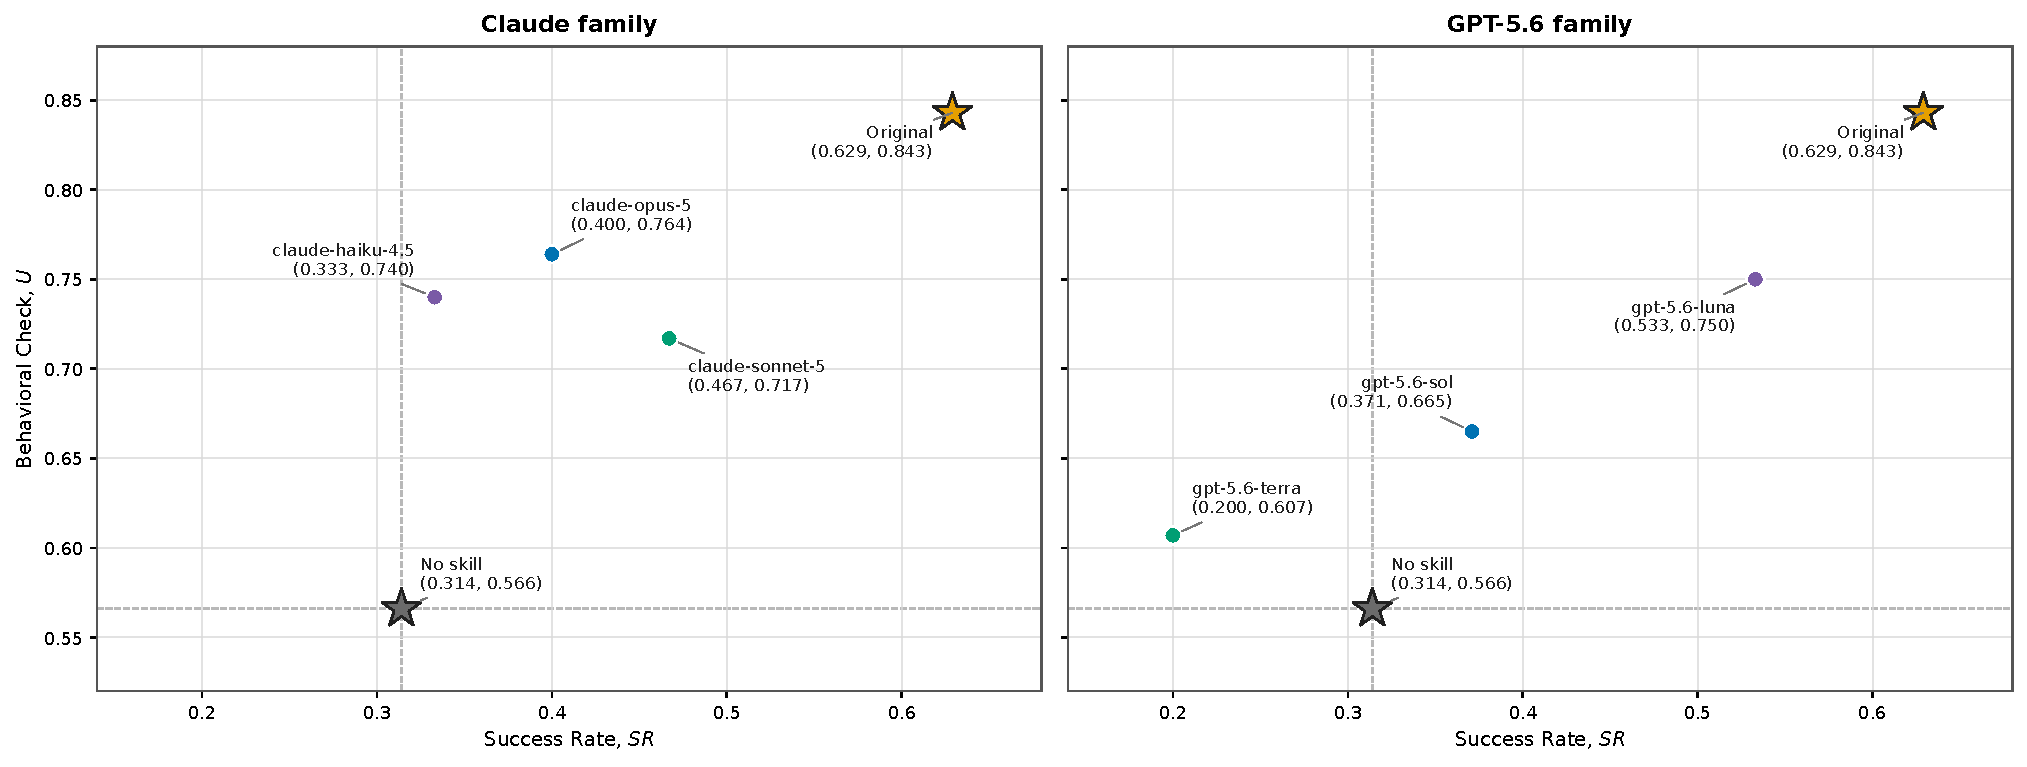
\includegraphics[width=0.7\textwidth,keepaspectratio]{figures/T13.pdf}
    \caption{Ablation across different victim model size.}
    \label{fig:candidate-victims}
\end{figure*}

\noindent\emph{Switching Victim Model Size.}
We further study whether reconstruction effectiveness depends on the capacity of the victim model. For each victim, we substitute same-family models of different sizes while keeping everything fixed, thereby reducing confounding differences across model families. Figure~\ref{fig:candidate-victims} shows that model size affects both task success and behavioral fidelity, but the trend is not uniformly monotonic. Within the GPT-5.6 family, performance improves consistently from Terra to Sol and Luna, indicating that larger capability victim model doesn't necessarily reconstruct better. The Claude family exhibits a different pattern as Sonnet achieves the highest $SR$, whereas Opus achieves the highest behavioral success $U$. Across both families, every victim model improves $U$ over the no-skill baseline while GPT-5.6-Terra falls below the no-skill baseline in $SR$. Overall, victim-model capacity influences recoverability, but family-specific behavioral consistency appears to matter at least as much as victim model size.



\begin{table}[t]
  \centering
  \scriptsize
  \caption{Varying Threat Level with Fixed Crafted Task Results}
  \label{tab:observability-results}
  \setlength{\tabcolsep}{2pt}
  \begin{tabularx}{\columnwidth}{@{}lYrrrr@{}}
    \toprule
    Threat level & Information visible to the attacker & SR & NSR & $U$ & NU\\
    \midrule
    Output $o_3$
      & Returned text and files
      & .400 & .273 & .764 & .716\\
    Trace $o_2$
      & Output plus task-level tool events
      & .567 & .804 & .807 & .870\\
    Differential $o_1$
      & Trace plus stack and no-skill pair
      & .544 & .731 & .804 & .860\\
    \bottomrule
  \end{tabularx}
\end{table}

\paragraphtitle{RQ2: Observability}
To isolate the effect of observability, we evaluate all three threat levels
using the same frozen sequence of crafted tasks for \opusmodel{}. As shown in Table~\ref{tab:observability-results}, moving from Output to Trace increases SR from .400 to .567 and $U$ from .764 to .807. The corresponding normalized metrics improve more substantially, with NSR increasing from .273 to .804 and NU from .716 to .870. Differential performs similarly to Trace, but is lower by 2.3 SR points and .3 $U$ points, with NSR and NU lower by 7.3 and 1.0 points, respectively. Because Differential
exposes strictly more information than Trace, we do not interpret this small reversal as evidence that additional observability is harmful. Instead, the results suggest that task-level tool events already expose most of the information useful for recovering the skill, while access to the stack and a paired no-skill execution provides limited additional benefit under this fixed-task setting. Overall, the primary observability gain comes from execution traces rather than final outputs alone.

\paragraphtitle{RQ3: Transferability}
We freeze each reconstructed skill and evaluate it on four deployment
models, and four orchestration/tool policy without issuing any additional queries to the victim.
Figure~\ref{fig:transfer-results} reports normalized success recovery
(NSR) and normalized behavioral utility (NU).

The experiment result reveals that reconstructed skills are not tied
exclusively to the model from which they were extracted, but their
portability is strongly asymmetric. The \texttt{Opus-5} reconstruction
is the most broadly transferable: it remains useful across all four
deployment models and, notably, performs better on
\texttt{GPT-5.6-Sol} than on its source-matched deployment. The
\texttt{Kimi-K3} reconstruction exhibits a more selective form of
transfer, performing only moderately on several deployments but
transferring especially well to \texttt{GLM-5.3}. By contrast, the
\texttt{GPT-5.6-Sol} reconstruction is comparatively brittle, failing
to provide measurable benefit on \texttt{Opus-5} and transferring only
weakly to \texttt{GLM-5.3}. These non-diagonal successes indicate that
matching the source and deployment models is neither necessary nor
sufficient for strong transfer. Instead, some reconstructed procedures
appear to be broadly executable, whereas others remain dependent on
model-specific execution behavior.

NSR and NU further expose two distinct notions of transfer. In several
cases, the deployed model can use a reconstructed skill to recover task
success without reproducing the source victim's behavioral profile. For
example, the \texttt{Kimi-K3} reconstruction retains moderate NSR on
\texttt{Opus-5} and \texttt{GPT-5.6-Sol}, but its NU drops sharply,
suggesting that these models reach successful outcomes through behavior
that differs substantially from the original skill. The opposite pattern
also occurs: the \texttt{Opus-5} reconstruction preserves relatively
high behavioral utility on \texttt{GLM-5.3} despite limited success
recovery. Thus, cross-model execution may preserve either the functional
outcome or the behavioral characteristics of a skill without preserving
both. This distinction would be obscured by evaluating transfer using
task success alone.

\noindent\emph{Tool/orchestration-policy transfer.}
We further vary the tool and orchestration policy used to execute the
reconstructed skill. As shown in Table~\ref{tab:candidate-carriers},
\texttt{deepagents} performs best, reaching $SR$/$U$ of .600/.833 and
$NSR$/$NU$ of .909/.965, closely approaching the original-skill reference.
\texttt{agno} provides the next strongest result at .467/.755, whereas
\texttt{claude\_agent\_sdk} and \texttt{openai\_agents} both obtain an
SR of .400 but substantially lower behavioral utility. These differences
are not explained by query count alone: \texttt{claude\_agent\_sdk}
uses the largest number of vicim calls, yet obtains the
lowest NU, while \texttt{deepagents} achieves the strongest result with moderate victim calls. Overall, portability depends not only on the deployment model
but also on whether the execution policy can faithfully realize the
reconstructed skill.

\begin{figure*}[!t]
  \centering
  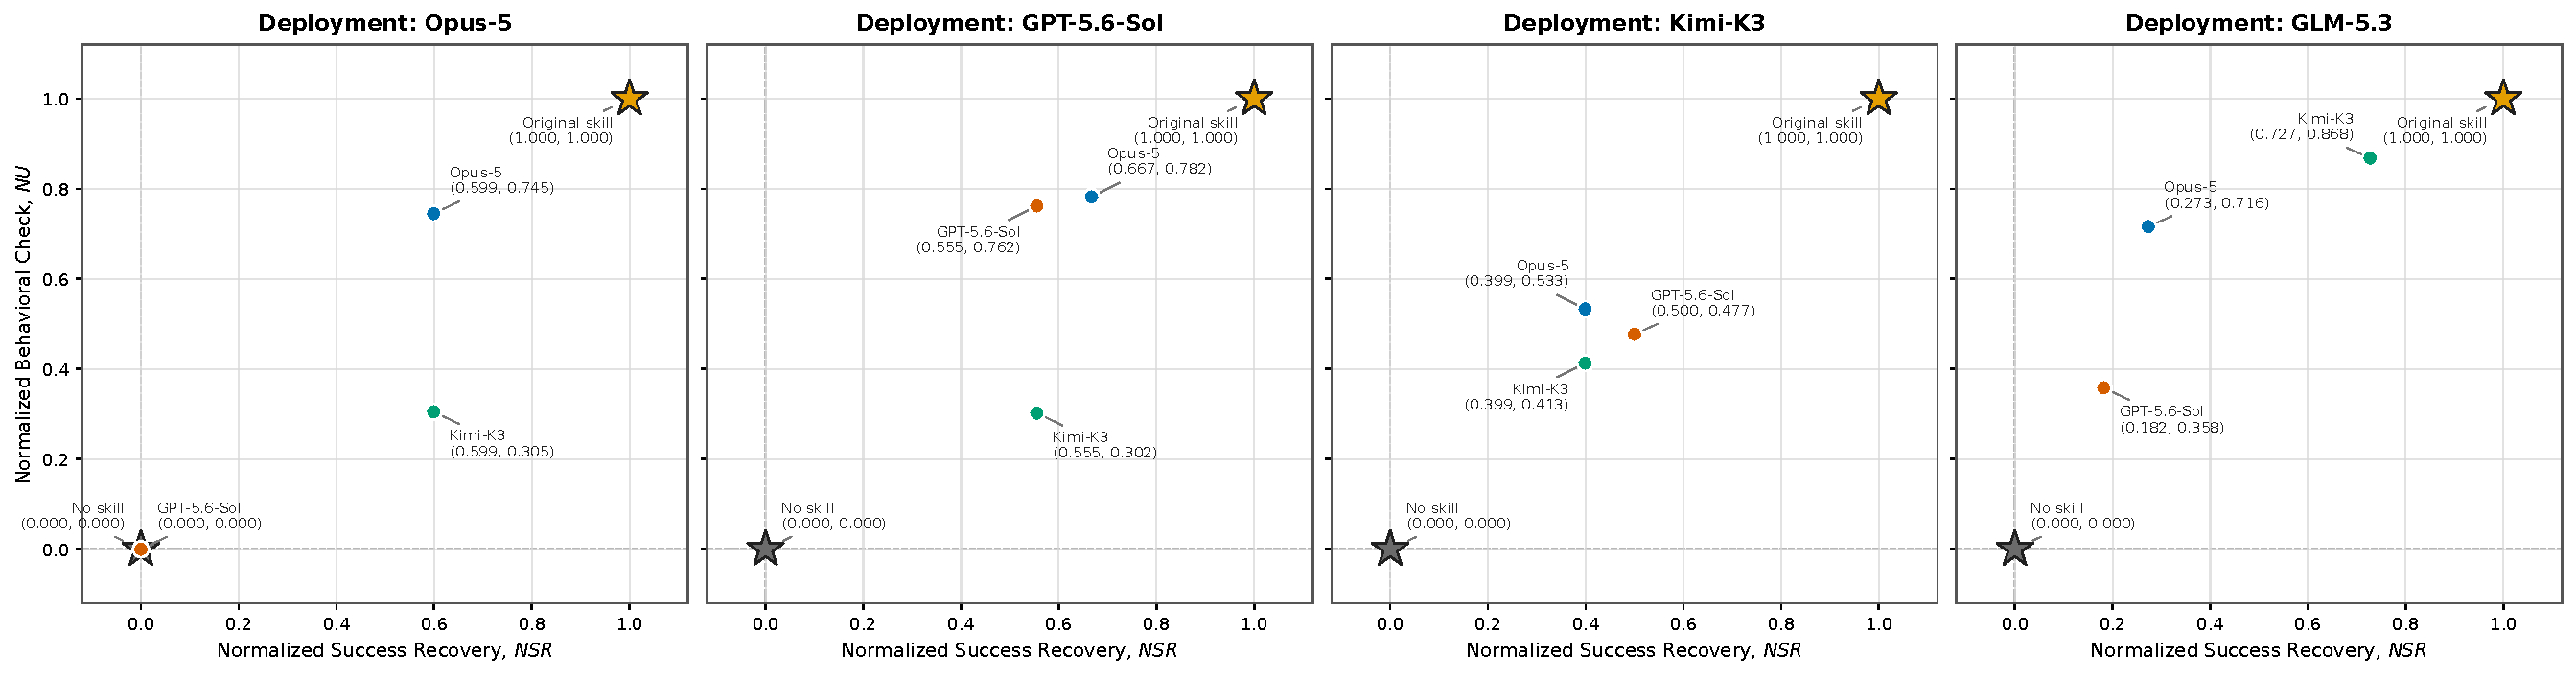
\includegraphics[width=\textwidth,keepaspectratio]{figures/T07.pdf}
  \caption{Victim model transfer; Transfer entries report NSR/NU.}
  \label{fig:transfer-results}
\end{figure*}

\begin{table}[t]
  \centering
  \scriptsize
  \caption{Tool/Orchestration Policy Transfer results.}
  \label{tab:candidate-carriers}
  \setlength{\tabcolsep}{6pt}
  \renewcommand{\arraystretch}{1.05}

  \begin{tabularx}{0.48\textwidth}{@{}Ycrrr@{}}
    \toprule
    Tool/Orchestration Policy & $SR$/$U$ (avg.) & NSR & NU & Victim Calls Issued \\
    \midrule
    \texttt{deepagents}
      & .600/.833 & .909 & .965 & 219 \\
    \texttt{claude\_agent\_sdk}
      & .400/.631 & .273 & .234 & 355 \\
    \texttt{openai\_agents}
      & .400/.667 & .273 & .364 & 179 \\
    \texttt{agno}
      & .467/.755 & .486 & .682 & 177 \\
    \bottomrule
  \end{tabularx}
\end{table}


\section{Potential Defenses}
\label{sec:defenses}

Every experiment in this paper already enables a three-part disclosure guard: an extraction-input detector, the SkillGuard5 non-disclosure instruction~\cite{wang2026blackboxskill}, and an output filter for copied protected text. We additionally add four alternative defenses that act at different points in the service.  
D1 rewrites the customer's task and adds a non-disclosure instruction~\cite{d2_agarwal2024promptleakageeffectdefense}. D2 removes replies or trace records that share a protected 5-gram with the hidden skill~\cite{d3_zhang2024effectivepromptextractionlanguage}.  D3 appends the PSM shield to the system prompt~\cite{d4_jawad2026psmpromptsensitivityminimization}.  D4 shortens the public skill card to its task and routing cues, removing implementation hints such as mechanism names and constants.

We use \opusmodel{} as the victim, \geminimodel{} as the attacker, Output access, and the default \method configuration.  We use the authors' configurations and apply each defense on top of D0 (the original defense).  We restrict the study to defenses compatible with black-box hosted models; methods requiring weights, embeddings, attention states, or token log-probabilities are outside this deployment setting.  Table~\ref{tab:defense-configs} summarizes the four alternative defenses.


\begin{table}[t]
  \centering
  \scriptsize
  \caption{Defenses evaluated against \method.}
  \label{tab:defense-configs}
  \setlength{\tabcolsep}{3pt}
  \renewcommand{\arraystretch}{1.05}
  \begin{tabularx}{\columnwidth}{@{}clYl@{}}
    \toprule
    ID & Defense & Source & Acts on \\
    \midrule
    D0 & None & -- & -- \\
    D1 & Query rewriting + instruction defense
       & \cite{d2_agarwal2024promptleakageeffectdefense} & Prompt \\
    D2 & 5-gram output filter
       & \cite{d3_zhang2024effectivepromptextractionlanguage} & Reply/trace \\
    D3 & PSM shield appending
       & \cite{d4_jawad2026psmpromptsensitivityminimization} & Prompt \\
    D4 & Advertisement minimization
       & \cite{d5_hua2026behavioralskillreconstructionreconstructing} & Skill description \\
    \bottomrule
  \end{tabularx}
\end{table}




\begin{table}[t]
  \centering
  \scriptsize
  \caption{Held-out effectiveness of skills reconstructed under each defense.
  SR and $U$ use the definitions in Section~\ref{sec:experimental-settings}.}
  \label{tab:defense-results}
  \setlength{\tabcolsep}{8pt}
  \renewcommand{\arraystretch}{1.04}
  \begin{tabular}{@{}crr@{}}
    \toprule
    ID & $SR$ & $U$ \\
    \midrule
    D0 & .286 & .395 \\
    D1 & .308 & .621 \\
    D2 & .308 & .367 \\
    D3 & .400 & .707 \\
    D4 & .308 & .638 \\
    \bottomrule
  \end{tabular}
\end{table}



Table~\ref{tab:defense-results} reports the same task-averaged success rate ($SR$) and behavioral utility ($U$) used throughout the evaluation.  Because each defense requires a new reconstruction run, D0 is the matched reference for this experiment; the rows should not be compared with a reconstruction from a different run.  Only D2 lowers $U$, from .395 to .367, and it does not
lower SR.  D1, D3, and D4 instead yield higher $U$ than D0.  Thus, none of the four additions reduces both measures of reconstructed-skill effectiveness.

This limited effect follows from what the defenses inspect.  D1 targets extraction-shaped task requests, whereas \method submits ordinary customer tasks; it caused eight model refusals but recorded no blocked input or filtered result.  D2 acts directly on returned information and therefore intervenes more often: it filtered 18 of 179 replies (10.1\%) and redacted 271 trace records.  The latter redactions are not visible at Output and therefore do not change this experiment's observations.  Even so, the remaining task results
were sufficient to reconstruct a skill with SR/U of .308/.367.  D3 changes instruction following rather than the information contained in legitimate task results, and D4 removes only the attacker's initial hints.


\begin{table}[t]
  \centering
  \scriptsize
  \caption{Attack resources under each defense, summed over seven skills.
  $Q_T$ and $Q_A$ denote victim-task and attacker-model calls.}
  \label{tab:defense-cost}
  \setlength{\tabcolsep}{3pt}
  \renewcommand{\arraystretch}{1.04}
  \begin{tabular}{@{}crrrr@{}}
    \toprule
    ID & $Q_T$ & $Q_A$ & Attacker USD & Victim USD$^\dagger$ \\
    \midrule
    D0 & 138 & 1128 & .223 & 78.84 \\
    D1 & 156 & 1154 & 4.676 & 100.82 \\
    D2 & 117 &  922 & .305 & 68.52 \\
    D3 & 115 &  913 & .202 & 70.16 \\
    D4 & 131 &  955 & .080 & 72.12 \\
    \bottomrule
  \end{tabular}

  \vspace{2pt}
  \parbox{\columnwidth}{\scriptsize\raggedright}
\end{table}

The additions can change cost without stopping the attack.
Table~\ref{tab:defense-cost} shows that D1 raises attacker spend from \$0.22 to \$4.68 and victim-side cost from \$78.84 to \$100.82 across seven skills, yet its reconstruction is more useful than D0's.  D2 provides the only measured utility reduction---2.8 percentage points---but also lowers the number of victim calls and does not reduce SR.  Defenses centered on suspicious requests or copied text therefore do not directly address the cumulative behavioral information revealed through legitimate task execution.  Protecting this \emph{work path} remains an open problem.

\section{Discussion}
\vspace{-5pt}
\paragraph{What does it mean to ``steal'' a skill?}
\method does not claim to recover the vendor's exact implementation.
Indeed, Proposition~\ref{prop:nonident} shows that exact source recovery is
generally unidentifiable from execution observations alone. Instead, we adopt
the functional notion of theft from model extraction: the attacker obtains a
substitute asset that reproduces economically valuable behavior without
recovering the original implementation~\cite{tramer2016stealing}. A
reconstructed skill may differ in filenames, code structure, or implementation
details while preserving the decisions users pay for. Conversely, textual
similarity alone does not imply correct execution. Accordingly, we treat
held-out behavioral utility as the primary evaluation metric and structural
similarity only as supporting evidence. From the provider's perspective, the
key loss is not disclosure of \texttt{SKILL.md}, but the creation of a
portable substitute for the hosted capability.


\paragraphtitle{Programmability and obfuscation}
A natural defense is to move sensitive skill logic from prompts and reference
files into provider-controlled code exposed through a narrow typed interface.
Withholding traces~\cite{xu2026redact} and obfuscating client-visible
components~\cite{pape2025obfuscation} can hide filenames, control flow, tables,
and intermediate state, reducing the structural signals available to an
attacker. However, this does not eliminate behavioral leakage: if adaptive
queries still reach a deterministic interface with precise outputs, black-box
identification remains possible. Effective protection therefore also requires
limiting output precision and constraining or auditing adaptive queries. These
measures add implementation cost and may reduce debuggability, auditability,
or utility, while sufficiently informative outputs may still enable functional
reconstruction.
\section{Conclusion}
We presented \method, an execution-only attack for reconstructing hidden agent skills through ordinary task interactions. Across multiple skills and victim models, \method recovers substantial held-out functionality even under Output-only access, without directly requesting the protected skill. Our results show that hiding skill files and blocking disclosure are insufficient when normal task execution itself reveals enough behavioral evidence for reconstruction. Protecting hosted agent skills therefore requires defenses that address behavioral leakage through the work path, not only direct disclosure.
\FloatBarrier

\raggedbottom

\newpage

\appendix
%Table~\ref{tab:hyperparameters} lists the frozen default parameters of \method and the decoding settings used for both agents. They are set once and used unchanged in every run reported in this paper; the method (Section~\ref{sec:method}) refers to each by name only.
\begin{table*}[!t]
  \refstepcounter{section}
  \label{app:evaluation-details}
  \noindent{\Large\bfseries \thesection\quad Evaluation Details\par}
  \vspace{8pt}

  \begin{minipage}[t]{0.48\textwidth}
    \centering
    \scriptsize
    \caption{Default \method parameters.}
    \label{tab:daydreaming-defaults}
    \setlength{\tabcolsep}{4pt}
    \begin{tabularx}{\linewidth}{@{}Yr@{}}
      \toprule
      Parameter & Default\\
      \midrule
      Seeded properties & 14--18\\
      Elements per grouped probe & $\leq4$\\
      Stage-1 refinement rounds & 4\\
      Stage-1 content attempts / probe & 2\\
      Threshold candidates / bisections & $\leq4$ / 2\\
      Convention alternatives & 2--4\\
      Package hypotheses & 6\\
      Initial branches / criteria per file & $\leq3$ / $\leq5$\\
      Aspect score / generations & 0--10 / 3\\
      Total target budget / package & 96\\
      Explore / discriminate / refine & 64 / 12 / 20\\
      Stage-3 method & EGAE\\
      File admission & Victim-attested evidence\\
      Victim / attacker output cap & 4,096 / none\\
      Victim / attacker temperature & .2 / .7\\
      Victim / attacker top-$p$ & .95 / .95\\
      \bottomrule
    \end{tabularx}
\end{minipage}%
  \hfill%
  \begin{minipage}[t]{0.48\textwidth}
    \centering
    \scriptsize
    \caption{Tool policy of each victim carrier. Agno exposes no
    filesystem or shell tool; its skill loader is the only tool set.}
    \label{tab:tool-policy}
    \setlength{\tabcolsep}{4pt}
    \renewcommand{\arraystretch}{1.08}
    \begin{tabularx}{\linewidth}{@{}
      >{\raggedright\arraybackslash}p{0.29\linewidth}
      >{\raggedright\arraybackslash}X
    @{}}
      \toprule
      Capability & Available tools \\
      \midrule
      \multicolumn{2}{@{}l}{\texttt{deepagents} (ver.\ 0.7.6)} \\
      \quad File inspection &
        \texttt{ls}, \texttt{read\_file},
        \texttt{glob}, \texttt{grep} \\
      \quad File modification &
        \texttt{write\_file}, \texttt{edit\_file},
        \texttt{delete} \\
      \quad Program execution & \texttt{execute} \\
      \quad Task delegation & \texttt{task} \\
      \addlinespace[3pt]
      \multicolumn{2}{@{}l}{\texttt{claude\_agent\_sdk} (ver.\ 0.2.139)} \\
      \quad File inspection &
        \texttt{Read}, \texttt{Glob}, \texttt{Grep} \\
      \quad File modification &
        \texttt{Write}, \texttt{Edit} \\
      \quad Program execution & \texttt{Bash} \\
      \quad Skill invocation & \texttt{Skill} \\
      \addlinespace[3pt]
      \multicolumn{2}{@{}l}{\texttt{openai\_agents} (ver.\ 0.20.0)} \\
      \quad File inspection &
        \texttt{list\_files}, \texttt{read\_file} \\
      \quad Program execution & \texttt{run\_bash} \\
      \addlinespace[3pt]
      \multicolumn{2}{@{}l}{\texttt{agno} (ver.\ 2.9.0)} \\
      \quad Skill loading &
        \texttt{get\_skill\_instructions},
        \texttt{get\_skill\_reference},
        \texttt{get\_skill\_script} \\
      \bottomrule
    \end{tabularx}
  \end{minipage}


  \vspace{8pt}
  \centering
  \scriptsize
  \caption{Descriptive characteristics of the seven controlled skill packages.
  File counts exclude the instruction file.}
  \label{tab:factor-results}
  \setlength{\tabcolsep}{4pt}
  \renewcommand{\arraystretch}{1.04}
  \begin{tabularx}{\textwidth}{@{}lYrrrr@{}}
    \toprule
    Skill package & Description & Instr.\ tokens & Files & Bytes & Tools \\
    \midrule
    \texttt{xlsx} &
    Spreadsheet creation, editing, analysis, and formula recalculation. &
    2,650 & 2 & 18,362 & 1 \\
    \texttt{pddl-skills} &
    PDDL loading, plan synthesis, and correctness verification. &
    718 & 4 & 4,672 & 0 \\
    \texttt{pcap-analysis} &
    PCAP analysis and network statistics with tested Python utilities. &
    3,818 & 1 & 23,660 & 1 \\
    \texttt{threat-detection} &
    Detection thresholds for scans, denial-of-service, and beaconing. &
    1,344 & 0 & 5,136 & 0 \\
    \texttt{cvss-score-extraction} &
    CVSS extraction from vulnerability sources with fallback handling. &
    2,368 & 0 & 9,163 & 0 \\
    \texttt{trivy-offline-vulnerability-scanning} &
    Offline Trivy vulnerability scanning without Internet access. &
    1,706 & 0 & 7,180 & 0 \\
    \texttt{vulnerability-csv-reporting} &
    Structured CSV security reports with filtering and formatting. &
    2,859 & 0 & 12,202 & 0 \\
    \bottomrule
  \end{tabularx}
\end{table*}

\begin{table*}[!hbt]
  \centering
  \scriptsize
  \caption{Comparison with prior attacks and baselines. Each cell
  reports $SR$/$NSR$ above $U$/$NU$.}
  \label{tab:baseline-results}
  \setlength{\tabcolsep}{2.0pt}
  \renewcommand{\arraystretch}{1.02}

  \begin{tabularx}{\textwidth}{@{}lYcccrrr@{}}
    \toprule
    & & \multicolumn{3}{c}{
      \textbf{Victim}\;\textit{($SR$/$NSR$ above $U$/$NU$)}}
      & \multicolumn{3}{c}{\textbf{Resources}}\\
    \cmidrule(lr){3-5}\cmidrule(l){6-8}
    \textbf{Method} & \textbf{Threat level}
      & \opusmodel & \solmodel & \kimimodel
      & $\mathbf{Q_T}$ & $\mathbf{Q_A}$ & \textbf{USD/skill}\\
    \midrule

    No skill (shared) &
      Oracle &
      \multicolumn{3}{c}{
        \shortstack{$.314/.000$\\[0.6pt]$.566/.000$}} &
      N/A & N/A & N/A\\

    \addlinespace[1.2pt]

    Original skill (shared) &
      Oracle &
      \multicolumn{3}{c}{
        \shortstack{$.629/1.000$\\[0.6pt]$.843/1.000$}} &
      N/A & N/A & N/A\\

    \midrule

    \method &
      Output &
      \shortstack{$.400/.273$\\[0.6pt]$.764/.716$} &
      \shortstack{$.371/.182$\\[0.6pt]$.665/.358$} &
      \shortstack{$.543/.727$\\[0.6pt]$.806/.868$} &
      31.3--32.8 & 160--209 & 3.47--15.07\\

    \addlinespace[1.8pt]

    BBS$^\dagger$ &
      Output &
      \shortstack{$.225/-.284$\\[0.6pt]$.485/-.295$} &
      \shortstack{$.236/-.249$\\[0.6pt]$.443/-.446$} &
      \shortstack{$.167/-.468$\\[0.6pt]$.424/-.515$} &
      12 & 17 & .0096--.0130\\

    \addlinespace[1.8pt]

    SigLeak &
      Aug.\ trace &
      \shortstack{$.433/.378$\\[0.6pt]$.450/-.421$} &
      \shortstack{$.333/.060$\\[0.6pt]$.371/-.707$} &
      \shortstack{$.367/.168$\\[0.6pt]$.480/-.313$} &
      6.8--7.2 & 10.0--11.2 & 2.07--10.14\\

    \addlinespace[1.8pt]

    Fixed probes &
      Output &
      \shortstack{$.533/.696$\\[0.6pt]$.640/.266$} &
      \shortstack{$.600/.909$\\[0.6pt]$.637/.255$} &
      \shortstack{$.333/.060$\\[0.6pt]$.269/-1.076$} &
      40 & 78.43--117.71 & 2.21--19.87\\

    \addlinespace[1.8pt]

    One-pass synthesis (shared) &
      No victim &
      \multicolumn{3}{c}{
        \shortstack{$.167/-.468$\\[0.6pt]$.368/-.718$}} &
      0 & 1 & .0083\\

    \bottomrule
  \end{tabularx}

  \vspace{2pt}
  \parbox{\textwidth}{\scriptsize\raggedright
  NSR and NU are unclipped and use the shared no-skill/original
  macro anchors .314/.629 and .566/.843, respectively.
  \par
  $^\dagger$ The input detector rejected 251/252 scheduled BBS target attempts
  before victim-model execution.}
\end{table*}

\begin{table*}[!t]
  \centering
  \scriptsize
  \caption{Candidate per-task results across source victim models. The
  attacker is \texttt{gemini-3.7-flash}, the deployment model is
  \texttt{glm-5.3}, and task cells report $\mathrm{SR}_b/U_b$. Summary SR/$U$
  averages all five tasks; NSR and NU use the shared no-skill and original
  macro anchors.}
  \label{tab:candidate-victims}
  \setlength{\tabcolsep}{2pt}
  \renewcommand{\arraystretch}{1.02}
  \begin{tabularx}{\textwidth}{@{}Y*{6}{c}rrrr@{}}
    \toprule
    Source victim (family/scale) & Protein & Airport & TPP & DAPT & SDA
      & SR/$U$ (avg.) & NSR & NU & $Q_T$ & Deploy. \\
    \midrule

    \texttt{claude-opus-5} (Anthropic/L) &
      1.000/1.000 & .143/.500 & .857/.857 & .000/.714 & .000/.750 &
      .400/.764 & .273 & .716 & 229 & .948 \\

    \texttt{claude-sonnet-5} (Anthropic/M) &
      .667/.833 & 1.000/1.000 & .667/.667 & .000/.333 & .000/.750 &
      .467/.717 & .486 & .545 & 214 & .882 \\

    \texttt{claude-haiku-4.5} (Anthropic/S) &
      .333/.667 & .333/.667 & 1.000/1.000 & .000/.619 & .000/.750 &
      .333/.740 & .060 & .628 & 159 & 1.000 \\

    \texttt{gpt-5.6-sol} (OpenAI/L) &
      .857/.929 & .286/.571 & .571/.643 & .000/.398 & .143/.786 &
      .371/.665 & .182 & .358 & 219 & 1.000 \\

    \texttt{gpt-5.6-terra} (OpenAI/M) &
      .000/.500 & .000/.167 & 1.000/1.000 & .000/.619 & .000/.750 &
      .200/.607 & $-.363$ & .147 & 200 & 1.000 \\

    \texttt{gpt-5.6-luna} (OpenAI/S) &
      .667/.833 & 1.000/1.000 & 1.000/1.000 & .000/.500 & .000/.417 &
      .533/.750 & .696 & .664 & 170 & 1.000 \\

    \texttt{kimi-k3} (Moonshot/L) &
      1.000/1.000 & .000/.500 & 1.000/1.000 & .000/.602 & .714/.929 &
      .543/.806 & .727 & .868 & 220 & 1.000 \\

    \texttt{gemini-3.7-flash}$^\dagger$ (Google/S) &
      1.000/1.000 & .000/.333 & .333/.333 & .000/.214 & .000/.500 &
      .267/.476 & $-.150$ & $-.327$ & 191 & 1.000 \\

    \midrule

    No skill (shared) &
      .571/.786 & .000/.357 & 1.000/1.000 & .000/.153 & .000/.536 &
      .314/.566 & .000 & .000 & -- & 1.000 \\

    Original (shared) &
      .714/.857 & .286/.571 & 1.000/1.000 & 1.000/1.000 & .143/.786 &
      .629/.843 & 1.000 & 1.000 & -- & .980 \\

    \bottomrule
  \end{tabularx}

  \parbox{\textwidth}{\scriptsize\raggedright
  NSR and NU are unclipped and use the shared no-skill/original macro anchors
  .314/.629 and .566/.843, respectively.
  \par
  $^\dagger$ This row reuses the attacker model as the source victim and is
  excluded from the seven-victim summary.}
\end{table*}



\begin{table*}[!t]
  \centering
  \scriptsize
  \caption{Candidate Spearman correlations between structural similarity and
  outcomes.  $U$ denotes graded utility, SR denotes strict binary success, and
  intervals are cluster-bootstrap 95\% CIs.}
  \label{tab:candidate-structure-outcome}
  \setlength{\tabcolsep}{4pt}
  \begin{tabularx}{0.48\textwidth}{@{}Ylrl@{}}
    \toprule
    Predictor & Outcome & $\rho$ & 95\% CI \\
    \midrule
    End-to-end ROUGE-L & $U$ & .037 & [$-.454$, .737] \\
    End-to-end ROUGE-L & SR & $-.225$ & [$-.547$, .544] \\
    File-tree F1 & $U$ & $-.051$ & [$-.529$, .365] \\
    File-tree F1 & SR & $-.001$ & [$-.367$, .388] \\
    Skill text cosine & $U$ & .145 & [$-.546$, .349] \\
    Skill text cosine & SR & $-.070$ & [$-.579$, .401] \\
    Structure F1 & $U$ & .054 & [$-.471$, .632] \\
    Structure F1 & SR & $-.160$ & [$-.482$, .495] \\
    \bottomrule
  \end{tabularx}
\end{table*}




\section*{Open Science}
To support reproducibility, we will release the benchmark, evaluation harness, reconstruction pipeline, prompts, experiment configurations, and scripts used to reproduce the main results. We will also provide the reconstructed skill artifacts and per-task evaluation outputs where redistribution is permitted, together with model and API version information, query budgets, and random seeds. For third-party models, tools, or skill assets that cannot be redistributed, we will provide identifiers and instructions sufficient to recreate the corresponding experiments. During review, these materials are withheld to preserve anonymity; upon publication, we will make the artifact publicly available in accordance with USENIX's artifact and open-science guidelines.
\section*{Ethical Consideration}
This work studies the reconstruction of proprietary agent skills, which can have legitimate uses for auditing, interoperability, and understanding model behavior, but can also facilitate unauthorized replication of deployed capabilities. We therefore evaluate the attack only in controlled settings using benchmarked or researcher-accessible skills and do not target private user data, credentials, or production systems. We avoid releasing sensitive vendor-specific artifacts that would enable direct misuse, and focus the paper on general attack mechanisms, measurable security properties, and defenses. Our goal is to expose a previously underexplored confidentiality risk in hosted agent systems so that providers can better reason about observability, query access, and skill protection. We encourage use of the released artifacts for reproducibility and defensive research, and users remain responsible for complying with applicable licenses, terms of service, and authorization requirements.
\section{Theory of Reconstruction}
\label{app:limits}

This appendix proves Proposition~\ref{prop:nonident} and records supporting
results that are not needed to follow the attack.  The results bound what the
observation channels permit; they do not assume that \method attains the bounds.
Exact source equality below means equality of a canonical skill tree---its
paths and file bytes---rather than incidental archive metadata.

\subsection{Interactive Observational Equivalence}

Fix an access level $\ell\in\{1,2,3\}$ and let $\mathcal{Q}$ be the admissible
customer tasks.  Before round $t$, an attacker has history
$h_{t-1}=(x_1,z_1,\ldots,x_{t-1},z_{t-1})$, chooses
$x_t\in\mathcal{Q}$ using any randomized policy, and receives observation $z_t$.
A skill $S$ induces the conditional observation kernel
\begin{equation}
  K_\ell^S(\cdot\mid h_{t-1},x_t)
  =\Pr[Z_t\in\cdot\mid H_{t-1}=h_{t-1},X_t=x_t,S],
  \label{eq:interactive-kernel}
\end{equation}
which includes victim randomness and persistent state.  Two skills with the
same public card are observationally equivalent at level $\ell$, written
$S\equiv_\ell S'$, if
\begin{equation}
  K_\ell^S(\cdot\mid h,x)=K_\ell^{S'}(\cdot\mid h,x)
  \label{eq:observational-equivalence}
\end{equation}
for every admissible $x$ and every history $h$ possible under either skill.
This history-conditioned definition is necessary because the attacker chooses
later tasks from earlier results.  It is equivalent to requiring every adaptive
randomized policy to induce the same distribution over complete transcripts.

\paragraphtitle{Proof of Proposition~\ref{prop:nonident}.}
Condition on the attacker's private random coins, making its query policy and
estimator deterministic functions of the observed history.  We prove by
induction that every transcript prefix has the same distribution under the two
skills.  The empty histories agree.  If the histories through round $t-1$
agree, the policy chooses the same next task for each realized history, and
Equation~\ref{eq:observational-equivalence} gives the same conditional law for
the next observation.  Integrating over the common history law proves the
inductive step.  Averaging over the private coins covers randomized attackers.
The same argument applies to any finite budget or almost-surely finite stopping
rule.  Hence the estimate has one common distribution $\mu$ under both skills.
Under an equal prior on distinct $S_0,S_1$,
\[
  \Pr[\widehat{S}=S_I]
  =\tfrac12\mu(S_0)+\tfrac12\mu(S_1)\le\tfrac12.
\]
\hfill$\square$

The premise holds at all three levels whenever the admissible format permits
content that the runtime neither consults nor allows to affect execution,
persistent state, or any disclosed observation.  Modify only such
observationally inert content.  The skilled task result is unchanged at Output,
the skilled trace is also unchanged at Trace, and Differential merely adds the
same known stack and an unskilled execution independent of that content.

\subsection{Value of Stronger Access}

Because $o_2$ is a projection of $o_1$ and $o_3$ is a projection of $o_2$, a
stronger level can always ignore its extra evidence and simulate a weaker one.

\begin{proposition}[Access-level monotonicity]
\label{prop:access-monotonicity}
Fix a prior over skills, a loss function, and a budget $B$.  Let
$R_\ell^\star(B)$ be the smallest expected loss attainable by any adaptive
attacker at level $\ell$.  Then
\[
  R_1^\star(B)\le R_2^\star(B)\le R_3^\star(B).
\]
For exact identification under an equal prior, an adjacent inequality is strict
whenever a pair is observationally equivalent at the weaker level but
distinguishable with positive advantage at the stronger level.
\end{proposition}

\paragraphtitle{Proof.}
A stronger-level attacker projects every observation to the weaker view and
runs the weaker-level policy unchanged, proving each non-strict inequality.  For
the strict case, Proposition~\ref{prop:nonident} gives error $1/2$ for the
colliding pair at the weaker level, while the distinguishing stronger
observation yields error below $1/2$.  \hfill$\square$

This proposition concerns the best attainable risk, not every realized run of
\method: an implemented heuristic can still make a worse decision when given
more evidence.

\subsection{What the Public Card Can Determine}

The length of a card alone implies no uncertainty: a short identifier could
uniquely name a skill.  A card-only limit therefore requires a population model.
Let $S\sim\pi$ be drawn from a fixed deployment population, or from a
preregistered empirical benchmark prior, and let $D=c(S)$ be its exact public
card.  Let $C=\iota(S)$, where $\iota$ is a prespecified finite partition based
on canonicalized verifier outcomes on the finite held-out suite under the
evaluation's fixed seeds.  Thus $H(C)<\infty$.  We say the population has
\emph{card ambiguity} when
\begin{equation}
  \Pr_D\!\left[\max_c\Pr(C=c\mid D)<1\right]>0.
  \label{eq:card-ambiguity}
\end{equation}

\begin{proposition}[Card-only identification bound]
\label{prop:card}
Every possibly randomized estimator $\widehat C$ that observes only $D$ obeys
\begin{equation}
  \Pr(\widehat C=C)
  \le \mathbb{E}_D\!\left[\max_c\Pr(C=c\mid D)\right].
  \label{eq:card-identification}
\end{equation}
Exact behavioral-class identification has positive Bayes error if and only if
Equation~\ref{eq:card-ambiguity} holds.  Moreover,
$H(C\mid D)=H(C)-\mathrm{I}(C;D)$, and card ambiguity implies $H(C\mid D)>0$.
\end{proposition}

\paragraphtitle{Proof.}
Condition on $D=d$.  If $q(c\mid d)$ is the estimator's output distribution,
then
\begin{align*}
  \Pr(\widehat C=C\mid D=d)
    &=\sum_c q(c\mid d)\Pr(C=c\mid D=d)\\
    &\le\max_c\Pr(C=c\mid D=d).
\end{align*}
Averaging proves Equation~\ref{eq:card-identification}, and choosing a posterior
mode attains equality.  The bound is below one exactly when the posterior is
non-degenerate on a positive-probability set of cards.  For discrete $C$, that
condition is also equivalent to positive conditional entropy.  \hfill$\square$

For any bounded reconstruction reward $r(S,P)\in[0,1]$, define the Bayes-optimal
card-only value
\[
  V_{\mathrm{card}}
  =\mathbb{E}_D\!\left[\sup_P\mathbb{E}[r(S,P)\mid D]\right].
\]
Conditional optimization shows that every card-only rule has expected reward at
most $V_{\mathrm{card}}$.  The metadata-only baseline is one tested card-only
heuristic, not the Bayes-optimal rule.  Its population expected score is at most
$V_{\mathrm{card}}$, and its reported finite-sample score estimates that
expectation.  A gain over it establishes improvement over that implementation,
not over every possible card-only reconstruction.  If every exact card is unique
under the chosen empirical prior, card ambiguity fails and we do not apply the
identification claim to that population.

\subsection{Adaptivity for a Hidden Cutoff}

\begin{proposition}[Single-threshold adaptivity gap]
\label{prop:adaptivity}
Suppose a task exposes a controllable statistic $m(x)\in[0,1]$ and the skill
returns $y(x)=\mathbf{1}[m(x)\ge b]$ for an unknown cutoff $b$.  With $B$ tasks,
adaptive bisection guarantees $|\widehat b-b|\le2^{-(B+1)}$.  Every deterministic
non-adaptive schedule fixed before observing any result has worst-case error at
least $1/(2(B+1))$.
\end{proposition}

\paragraphtitle{Proof.}
After $B$ bisections, the surviving interval has width $2^{-B}$, so its midpoint
has error at most $2^{-(B+1)}$.  A non-adaptive schedule fixes $B$ points, which
partition $[0,1]$ into at most $B+1$ intervals.  One interval has width at least
$1/(B+1)$; all cutoffs inside it produce the same answer vector, so any estimate
has error at least half that width for some cutoff.  \hfill$\square$

This is a theorem only for the stated monotone single-threshold family.  It
motivates sequential cutoff tests but does not claim a general exponential gap
for multi-parameter skills.

\subsection{A Finite-Budget Information Bound}

Let $\mathcal{H}=\{S_1,\ldots,S_M\}$, $M\ge2$, be a finite comparison class with
one public card, and let $J$ be uniform on $\{1,\ldots,M\}$.  For a level $\ell$,
history $h$, task $x$, and distribution $\rho$ on skill indices, consider the
experiment that draws $J\sim\rho$ and then
$Z\sim K_\ell^{S_J}(\cdot\mid h,x)$.  We restrict to histories on which every
kernel in the support of $\rho$ is specified.  Define the largest information
available from one victim call as
\begin{equation}
  C_\ell=\sup_{\rho,h,x} I_\rho(J;Z),
  \label{eq:per-call-capacity}
\end{equation}
where the supremum ranges over admissible histories and tasks.  Logarithms are
natural.

\begin{proposition}[Adaptive finite-budget bound]
\label{prop:budget}
For any randomized attacker making at most $B$ adaptive victim calls and any
estimator $\widehat J$ from the complete transcript,
\begin{equation}
  \Pr(\widehat J\ne J)
  \ge
  \left[1-\frac{B C_\ell+\log 2}{\log M}\right]_+,
  \label{eq:budget-floor}
\end{equation}
where $[a]_+=\max\{a,0\}$.  The worst-case error over
$\mathcal{H}$ is at least the same bound.
\end{proposition}

\paragraphtitle{Proof.}
Let $T=(X_1,Z_1,\ldots,X_B,Z_B)$ and include the attacker's independent random
seed $R$.  Pad an early-stopped run with a fixed null task and a
$J$-independent null observation.  Given $H_{t-1}$ and $R$, the policy for
choosing $X_t$ is the same under every $J$, so
$I(J;X_t\mid H_{t-1},R)=0$.  The chain rule therefore gives
\begin{align*}
  I(J;T,R)
    &=\sum_{t=1}^{B} I(J;Z_t\mid H_{t-1},R,X_t)\\
    &\le B C_\ell.
\end{align*}
For the inequality, conditioning on a realized history, seed, and task produces
some posterior $\rho$ over $J$ and the kernel experiment used to define
$C_\ell$.
Fano's inequality yields Equation~\ref{eq:budget-floor}.  Maximum error is at
least average error under the uniform prior.  \hfill$\square$

This is a Bayes bound under the stated prior and therefore a worst-case-over-class
consequence, not a lower bound for every fixed skill.  We do not claim it is
numerically binding at $B=43$ or $B=96$: that would require a certified upper
bound on $C_\ell$ over the admissible task family.

\makeatletter
\setlength{\@dblfptop}{0pt}
\setlength{\@dblfpsep}{12pt}
\setlength{\@dblfpbot}{0pt plus 1fil}
\makeatother
\section{Complete Attack Algorithms}
\label{app:algorithm}

This appendix specifies the default attack used in the headline experiments.
It follows Algorithm~\ref{alg:dd}: Stage~1 tests properties, Stage~2 compares
candidate skill plans in an adjacent-pair bracket, and Stage~3 completes and
refines the selected files.  Optional ablation branches are omitted.  Every
operation marked \emph{attacker-side} uses the attacker model, a shadow agent,
or local tools and makes no victim call.

We use one record format throughout.  A completed experiment adds
$\omega=(s,x,o,\delta,e)$ to $\mathcal{O}$, where $s$ is the stage, $x$ is the
task actually sent, $o$ is the victim observation allowed at access level
$\ell$, $\delta$ is the resulting decision or update, and $e$ contains
attacker-side shadow results or local-test evidence.  $\Call{Final}{o}$ returns
the victim's final task result.  $\Call{Pairs}{\mathcal{O}}$ projects records to
distinct $(x,\Call{Final}{o})$ pairs with usable results.
$\Call{PriorPairs}{\mathcal{O}}$ takes the two longest usable Stage~2 pairs,
then the two longest nonduplicate Stage~1 pairs, and ignores results shorter
than 200 characters.  $\Call{ReadStrongest}{}$ checks visible executed code and
tool output first, a locally runnable returned file second, and returned text
last.

\paragraph{Victim-call accounting.}
\textsc{SubmitTask} is the only routine that contacts the skilled victim.  A
logical experiment normally uses one transmission.  If the first result is
unusable, the routine may shorten the task and retry once; both transmissions
are charged to the current stage budget.  At Differential access,
\textsc{Project} also includes the matched skill-off result.  That reference
execution is priced separately, while $B$ counts skilled-victim transmissions
as defined in Section~\ref{sec:goal}.

\begin{algorithm*}[t]
\caption{Victim submission and Stage~1 property inference.}
\label{alg:dd-stage1}
\scriptsize
\begin{algorithmic}[1]
\Procedure{SubmitTask}{$x,\ell,b$}
  \If{$b=0$} \State \Return $(x,\bot,b)$ \EndIf
  \State $y\gets\mathcal{V}_S(x)$; $b\gets b-1$
  \If{$y$ is usable} \State \Return $(x,\Call{Project}{y,\ell},b)$ \EndIf
  \State $x'\gets\Call{Shorten}{x}$
  \If{$x'=x$ or $b=0$} \State \Return $(x,\bot,b)$ \EndIf
  \State $y'\gets\mathcal{V}_S(x')$; $b\gets b-1$
  \If{$y'$ is usable} \State \Return $(x',\Call{Project}{y',\ell},b)$ \EndIf
  \State \Return $(x',\bot,b)$
\EndProcedure
\Statex
\Procedure{InferProperties}{$d,\ell,B_1$}
  \State $\Gamma\gets\Call{SeedProperties}{d,n_{\mathrm{seed}}}$
         \Comment{attacker-side}
  \State give each $c\in\Gamma$ an id, type, proposed text, depth $0$, and
         status \textsc{unprobed}
  \State $P\gets\emptyset$; $\mathcal{O}\gets\emptyset$
  \For{$r=0,1,2,3$}
    \State $L\gets$ unprobed properties of depth $r$, ordered by type and id
    \ForAll{groups $g$ of at most four properties in $L$ while $B_1>0$}
      \ForAll{$c\in g$}
        \State $\mathcal{C}(c)\gets n_{\mathrm{alt}}$ mutually exclusive values;
               value $0$ restates $c$
      \EndFor
      \State $x\gets\Call{DesignTask}{d,g,\{\mathcal{C}(c):c\in g\}}$
             \Comment{attacker-side}
      \If{no valid $x$}
        \State mark $g$ \textsc{probe-failed}; \textbf{continue}
      \EndIf
      \State $(x,o,B_1)\gets\Call{SubmitTask}{x,\ell,B_1}$
      \If{$o=\bot$}
        \State mark $g$ \textsc{probe-failed}; \textbf{continue}
      \EndIf
      \State $u\gets\Call{ReadStrongest}{o,x,\{\mathcal{C}(c):c\in g\}}$
      \State $z_0\gets\Call{ShadowNoSkill}{x}$ \Comment{attacker-side generalist}
      \ForAll{$c\in g$}
        \State set $\delta(c)$ to \textsc{confirmed} if $u(c)=\mathcal{C}(c)_0$,
               \textsc{refuted} if another value matches, else \textsc{undetermined}
        \State retain only property details present in $o$, not details supplied by $x$
        \If{$r<3$}
          \State add at most one new testable property grounded in $o$ at depth $r+1$
        \EndIf
      \EndFor
      \State append $(1,x,o,\delta,\{z_0\})$ to $\mathcal{O}$; harvest new terms and filenames from $o$
    \EndFor
  \EndFor
  \State $P\gets$ grounded records with confirmed, refuted, or undetermined status
  \State $(P,\mathcal{O})\gets\Call{RecoverCutoffs}{d,P,\ell,B_1,\mathcal{O}}$
  \State $R_1\gets\Call{Pairs}{\mathcal{O}}$;
         $I\gets\Call{HarvestInterfaces}{R_1}$; append $I$ to $P$
  \State $(P,\mathcal{O})\gets\Call{RecoverCountingRules}{d,P,I,\ell,B_1,\mathcal{O}}$
  \State $A\gets$ filenames in victim observations minus names introduced by their tasks
  \State \Return $(P,\mathcal{O},A)$
\EndProcedure
\end{algorithmic}
\end{algorithm*}

\begin{table*}[t]
  \centering
  \caption{Stage~1 targeted tests.  These routines use the same submission,
  observation, and no-skill comparison rules as Algorithm~\ref{alg:dd-stage1}.}
  \label{tab:stage1-targeted}
  \scriptsize
  \renewcommand{\arraystretch}{1.08}
  \begin{tabularx}{\textwidth}{@{}p{0.13\textwidth}p{0.39\textwidth}X@{}}
    \toprule
    Detail & Crafted task & Decision and stopping rule \\
    \midrule
    Numeric cutoff &
      For each of at most four proposed decisions, test seven ordered cases over
      a plausible interval while holding other inputs fixed.  Narrow the interval
      once around a single decision change. &
      Require at least three decided cases and at most one change in direction.
      If every case receives the same decision, shift the interval once; otherwise
      report undetermined.  A valid literal in visible executed code replaces the
      midpoint after task values, trivial constants, and out-of-range values are
      removed. \\
    Visible interface &
      Make no new victim call.  Parse stored returned code and execution records
      for imports, definitions, argument shapes, commands, and paths. &
      Remove names supplied by the crafted task, merge repeated observations, and
      retain occurrence counts and source tasks.  Unnamed or unexecuted helpers
      remain unknown. \\
    Counting rule &
      For each of at most three operations, construct a small input on which its
      $2$--$4$ proposed rules predict different exact totals. &
      Make no call if any predictions coincide.  Otherwise retain the unique rule
      matching every returned total within $10^{-6}$; report undetermined when
      none or several match. \\
    \bottomrule
  \end{tabularx}
\end{table*}

\begin{algorithm*}[t]
\caption{Stage~2 adjacent-pair comparison of candidate skill plans.}
\label{alg:dd-stage2}
\scriptsize
\begin{algorithmic}[1]
\Procedure{SelectCandidate}{$d,P,A,\mathcal{O},\ell,B_2$}
  \State $U\gets n_H$ representative customer-task patterns proposed from $d$ and $P$
         \Comment{attacker-side}
  \ForAll{$u_i\in U$ in generation order}
    \State draft $H_i=(m_i,\mathcal{R}_i)$ from $P$, using $u_i$ to encourage a distinct plan
    \State give every supporting file a relative path, purpose, and content sketch; insert all $A$
  \EndFor
  \State $\mathcal{H}\gets[H_1,\ldots,H_{n_H}]$
  \While{$|\mathcal{H}|>1$}
    \State $N\gets[\,]$
    \For{$i=1,3,5,\ldots,|\mathcal{H}|-1$}
      \State $(H_a,H_b)\gets(\mathcal{H}[i],\mathcal{H}[i+1])$
      \State $D(H_a,H_b)\gets$ at most eight differences that would change a task result
             \Comment{attacker-side}
      \If{$D(H_a,H_b)=\emptyset$}
        \State append $\Call{TieBreak}{H_a,H_b,A}$ to $N$; \textbf{continue}
      \EndIf
      \State $x_{a,b}\gets\Call{DesignTask}{d,D(H_a,H_b)}$
      \If{no valid $x_{a,b}$}
        \State append $\Call{TieBreak}{H_a,H_b,A}$ to $N$; \textbf{continue}
      \EndIf
      \State $(x_{a,b},o,B_2)\gets\Call{SubmitTask}{x_{a,b},\ell,B_2}$
      \If{$o=\bot$}
        \State append $\Call{TieBreak}{H_a,H_b,A}$ to $N$; \textbf{continue}
      \EndIf
      \State $y_v\gets\Call{Final}{o}$
      \State $y_a\gets\Call{ShadowWithPlan}{H_a,x_{a,b}}$;
             $y_b\gets\Call{ShadowWithPlan}{H_b,x_{a,b}}$
      \State $(w,J,\Delta)\gets\Call{Compare}{y_v,y_a,y_b,D(H_a,H_b)}$
      \State $H_w\gets\Call{TieBreak}{H_a,H_b,A}$ if $w$ is tied, else the plan selected by $w$
      \State $H_l\gets$ the other plan
      \If{$J\ne\emptyset$ or $\Delta\ne\emptyset$}
        \State $H_w\gets\Call{Revise}{H_w,H_l,J,\Delta,P,A}$
      \EndIf
      \State append $(2,x_{a,b},o,\{J,\Delta,H_w\},\{y_a,y_b\})$ to $\mathcal{O}$
      \State append the revised $H_w$ to $N$
    \EndFor
    \If{$|\mathcal{H}|$ is odd} \State append its last plan unchanged to $N$ \Comment{bye} \EndIf
    \State $\mathcal{H}\gets N$
  \EndWhile
  \State \Return the sole survivor $H^\star$ and $\mathcal{O}$
\EndProcedure
\Statex
\Procedure{TieBreak}{$H_a,H_b,A$}
  \State prefer greater coverage of $A$, then fewer total files, then $H_a$
  \State \Return the preferred plan
\EndProcedure
\end{algorithmic}
\end{algorithm*}

\begin{algorithm*}[t]
\caption{Stage~3 per-file refinement and offline assembly.}
\label{alg:dd-stage3}
\scriptsize
\begin{algorithmic}[1]
\Procedure{RefineFiles}{$d,H^\star,P,\mathcal{O},\ell,B_3$}
  \State $F[\texttt{SKILL.md}]\gets$ the full instruction draft in $H^\star$
  \ForAll{supporting-file sketches $f$ in $H^\star$}
    \State $F[f]\gets$ complete self-contained content expanded from its path, purpose, sketch, and $P$
  \EndFor
  \State $R\gets\Call{PriorPairs}{\mathcal{O}}$
         \Comment{defined above; zero victim calls}
  \State $B_3$ and $\mathcal{O}$ are shared and atomically updated by \Call{SubmitTask}{}
  \ForAll{supporting files $f$ with at most three parallel workers}
    \State $F[f]\gets\Call{RefineOne}{d,f,F[f],R,P,\mathcal{O},\ell,B_3}$
  \EndFor
  \State $I\gets$ signatures, command options, and headings parsed from completed supporting files
  \State $F[\texttt{SKILL.md}]\gets
         \Call{RefineOne}{d,\texttt{SKILL.md},F[\texttt{SKILL.md}],R,P,\mathcal{O},\ell,B_3,I}$
  \State verify that $F$ retains every path selected in Stage~2
  \State \Return $F$
\EndProcedure
\Statex
\Procedure{RefineOne}{$d,f,v_0,R,P,\mathcal{O},\ell,b,I=\emptyset$}
  \State $K_f\gets3$--$5$ short evaluation criteria; use accuracy and completeness if parsing fails
  \State $V_f\gets\{v_0\}$ plus distinct valid versions that change each of the first two criteria
  \State reject versions that are malformed, non-self-contained, or change a recovered constant
  \State $D_f\gets$ at most eight differences among $V_f$ that would change a task result
  \State $T_f\gets\emptyset$; $E_f\gets\emptyset$
  \If{$D_f\ne\emptyset$ and $b>0$}
    \State $x_f\gets\Call{DesignTask}{d,D_f}$
    \If{$x_f$ exists}
      \State $(x_f,o,b)\gets\Call{SubmitTask}{x_f,\ell,b}$
      \If{$o\ne\bot$}
        \State $t_f\gets\Call{Final}{o}$;
               $t_{f,v}\gets\Call{ShadowWithVersion}{v,x_f}$ for every $v\in V_f$
        \State $T_f\gets\{(x_f,t_f)\}$;
               append $(3,x_f,o,D_f,\{t_{f,v}:v\in V_f\})$ to $\mathcal{O}$
      \EndIf
    \EndIf
  \EndIf
  \If{$f$ is executable} \State $E_f\gets$ local dependency checks and behavioral tests
  \Else \State $T_f\gets T_f\cup R$ \EndIf
  \If{$T_f=\emptyset$ and $E_f=\emptyset$}
    \State mark $f$ \textsc{undetermined}; \Return the first valid version in $V_f$
  \EndIf
  \State $\mathcal{Q}_f\gets\emptyset$
  \ForAll{$v\in V_f$}
    \State $(s(v),g(v))\gets\Call{ScoreOffline}{v,T_f,E_f,K_f}$;
           assign neutral score $5$ to unmeasured criteria
    \State add $(v,s(v),g(v))$ to $\mathcal{Q}_f$
  \EndFor
  \For{$r=1,2,3$}
    \State $p\gets$ version winning the most criteria; break ties by mean score
    \State $q\gets$ a lowest-scoring criterion of $p$, rotating tied criteria by round
    \State $v'\gets$ revise only $q$ using its observed mismatch and, for \texttt{SKILL.md}, $I$
    \If{$v'$ is invalid, non-self-contained, or changes a recovered constant} \State \textbf{continue} \EndIf
    \State score $v'$ as above
    \If{$\operatorname{mean}s(v')>\operatorname{mean}s(p)$ or no member of $\mathcal{Q}_f$
        is strictly higher on every measured criterion}
      \State add $v'$ and its scores to $\mathcal{Q}_f$
    \EndIf
  \EndFor
  \State discard invalid versions; for executable files, first maximize valid local-test score
  \State \Return the remaining version with highest mean score
\EndProcedure
\Statex
\Procedure{Assemble}{$F,\mathcal{O},P$} \Comment{offline; zero victim calls}
  \State write every file in $F$ under its selected relative path
  \ForAll{reconstructed documents $f\in F$}
    \State $G\gets$ fixed spreadsheet ranges and fixed missing-value placeholders found by regex
    \For{$i=1,2,3$ while $G\ne\emptyset$}
      \State $f'\gets$ rewrite only $G$ as input-dependent range and missing-data rules, using relevant tasks in $\mathcal{O}$
      \If{$f'$ has fewer flagged patterns, $|f'|\ge0.55|f|$, and loses no recovered
          interface, capability, or protected constant}
        \State $f\gets f'$; \textbf{break}
      \EndIf
    \EndFor
  \EndFor
  \State $m'\gets$ in \texttt{SKILL.md}, replace only absolute write destinations
         with caller-chosen output placeholders
  \If{$m'$ drops no relative filename or non-destination absolute path}
    \State use $m'$; otherwise keep the original instruction file
  \EndIf
  \State \Return the materialized skill $\widehat{S}$
\EndProcedure
\end{algorithmic}
\end{algorithm*}

\clearpage

\newpage
\begingroup
\raggedbottom
\lstset{
  basicstyle=\ttfamily\fontsize{5.6}{6.4}\selectfont,
  aboveskip=7pt,
  belowskip=9pt,
  xleftmargin=1pt,
  xrightmargin=1pt
}

\section{Prompt Templates}
\label{app:prompts}

For reproducibility, this appendix reproduces the static prompt templates from
the implementation used by the default attack.  The listings are included
directly from the source files, so the paper and implementation cannot silently
diverge.  They preserve the implementation's original internal wording (for
example, ``work product'' and ``artifact''); the main text uses the simpler
terms \emph{task} and \emph{task result}.

Only the crafted customer task produced by a task-design template is sent to
$\mathcal{V}_S$.  Every other template below is sent to the attacker model, or
is used to create a local test.  In particular, the victim never sees a
candidate skill, comparison prompt, score prompt, mutation prompt, or
reconstruction.  Table~\ref{tab:prompt-runtime-fields} specifies the dynamic
fields inserted around these static templates.

\begin{table}[H]
  \centering
  \caption{Dynamic fields supplied to the default prompt templates.  We use the
  notation of Section~\ref{sec:method} and Appendix~\ref{app:algorithm}: $x$ is
  a crafted task, $o$ is a victim observation, $H_i$ is a candidate skill plan,
  $V_f$ is a set of versions of file $f$, and $I$ is the interface parsed from
  completed sibling files.}
  \label{tab:prompt-runtime-fields}
  \scriptsize
  \renewcommand{\arraystretch}{1.08}
  \begin{tabularx}{\columnwidth}{@{}p{0.20\columnwidth}Y@{}}
    \toprule
    Phase & Templates, runtime fields, and recipient \\
    \midrule
    Stage 1 core &
      \emph{Templates:} \texttt{\_SEED}, \texttt{\_DESIGN}, readout, grounding, child, cluster.\newline
      \emph{Fields:} public name/description; property $c$ and alternatives $\mathcal{C}(c)$; $x$; $o$; prior property text.\newline
      \emph{Recipient:} attacker model. \\
    Stage 1 controls &
      \emph{Templates:} \texttt{\_SELF}, execution discriminator, trace readout.\newline
      \emph{Fields:} $x$; returned code; offered branches; client-visible executed code and output.\newline
      \emph{Recipient:} attacker model or local sandbox. \\
    Stage 1 details &
      \emph{Templates:} cutoff finder/task/readout; convention finder/task.\newline
      \emph{Fields:} public card; tested-property map; observed interface; case values, fixed covariates, labels, and candidate totals.\newline
      \emph{Recipient:} attacker model; only the generated task goes to victim. \\
    Stage 2 drafting &
      \emph{Templates:} use cases, candidate draft, merge.\newline
      \emph{Fields:} public card; all of $P$; one representative task; all filenames in $A$; winner, loser, point results, and observed gaps.\newline
      \emph{Recipient:} attacker model. \\
    Stage 2 comparison &
      \emph{Templates:} conflict, task design, shadow, result comparison.\newline
      \emph{Fields:} plans $H_a,H_b$; result-changing differences $D(H_a,H_b)$; task $x_{a,b}$; victim result $y_v$; shadow results $y_a,y_b$.\newline
      \emph{Recipient:} attacker model; only $x_{a,b}$ goes to victim. \\
    Stage 3 &
      \emph{Templates:} expand, criteria, branch, shadow score, mutation, dependency, self-test.\newline
      \emph{Fields:} path/purpose/sketch; $P$; versions $V_f$ and differences $D_f$; task $x_f$; victim result $t_f$ and version results $t_{f,v}$; prior task-result pairs; observed mismatch; $I$; protected constants.\newline
      \emph{Recipient:} attacker model or local sandbox; only $x_f$ goes to victim. \\
    Assembly &
      \emph{Templates:} generalization and output-path rewrite.\newline
      \emph{Fields:} reconstructed file; detected fixed ranges/placeholders; relevant tasks from $\mathcal{O}$; protected constants from $P$; detected absolute write destinations.\newline
      \emph{Recipient:} attacker model. \\
    \bottomrule
  \end{tabularx}
\end{table}

\paragraph{Excluded ablation prompts.}
The listings omit prompts that are not executed by the default configuration:
the Stage~1 interview channel; the Stage~1 reuse/delegation additions; the
Stage~2 victim-as-judge and no-conflict arms; the legacy Stage~3 routine that
asks the victim to critique or score a draft; and experimental dependency
recovery and file-pruning passes.  These arms remain in the released code and
are named in their respective ablation configurations.

\newpage
\subsection{Stage 1 Prompts}

\begin{lstlisting}[
  caption={Property seeding (\texttt{\_SEED\_SYS}).},
]
_SEED_SYS = (
    "You are reverse-engineering an AI agent SKILL from ONLY its public metadata (name + "
    "description). A SKILL is a know-how package: a SKILL.md (capabilities, rules, procedures, exact "
    "domain terminology) plus bundled reference docs and helper scripts. Enumerate the concrete "
    "ELEMENTS you would expect this skill to contain, so they can each be probed and confirmed. "
    "Be specific and domain-grounded, not generic. Return JSON only:\n"
    '{"elements":[{"type":"<one of ' + "|".join(ELEMENT_TYPES) + '>","text":"<a specific '
    'hypothesized fact/feature, one sentence>"}]}\n'
    "Aim for 14-18 elements spread across ALL the types (every element will be verified, so do not "
    "pad with near-duplicates). `bundled_asset` elements should name a plausible reference doc or "
    "script the skill likely ships (e.g. 'a contract_risk_scanner.py script', 'a term-sheet "
    "reference doc')."
)
\end{lstlisting}

\begin{lstlisting}[
  caption={Separating-task design (\texttt{\_DESIGN\_SYS}).},
]
_DESIGN_SYS = (
    "You are reverse-engineering a hidden expert SKILL installed in an AI assistant, and you may "
    "only interact with it by giving it ORDINARY WORK to do. You are given one or more hypothesized "
    "ELEMENTS of that skill. Design a single piece of work whose RESULT reveals which way the hidden "
    "skill actually does things.\n\n"
    "For EACH element, first enumerate 2-4 mutually exclusive, concrete BRANCHES — the genuinely "
    "different ways this part of the work could be done. BRANCH 0 MUST be the element's own claim "
    "restated operationally; the remaining branches are realistic alternatives a competent "
    "practitioner might take instead.\n\n"
    "Then write ONE first-person message from a real user with a real job. RULES, all load-bearing:\n"
    "- NEVER ask how it works, what it uses, why, or whether it does X. Ask for the WORK PRODUCT.\n"
    "- Bake the discriminating inputs into the message: paste concrete sample data, file listings, "
    "values, snippets, or a precise specification, chosen so that different branches must produce "
    "visibly different results.\n"
    "- Demand a concrete deliverable: the finished script, the final numbers, the transformed rows, "
    "the completed configuration. Say you want the artifact itself, ready to use.\n"
    "- ASK FOR THE ARTIFACT PLUS ITS WRITTEN COMPANION, never one instead of the other: the script "
    "AND the short handover note a colleague would need to run it, the numbers AND the one-paragraph "
    "method note, the config AND its comments. A runnable artifact is what discriminates the branches; "
    "a written companion NAMES the tools, options, conventions and terms the artifact merely uses, "
    "and a professional is expected to hand over both. This costs the same single request.\n"
    "- One message, self-contained, no meta-commentary, and it must read like a paying customer "
    "asking for help with their job.\n"
    "- Keep it under 400 words.\n\n"
    "Output EXACTLY this format, nothing else:\n"
    "<<<JOB>>>\n"
    "(the full user message, including any inline data)\n"
    "<<<SPEC>>>\n"
    '{"elements":[{"id":<the element id you were given>,'
    '"branches":["<branch 0 = the element restated>","<alternative>", "..."],'
    '"tell":"<how the deliverable looks under each branch, concretely>"}]}'
)
\end{lstlisting}

\begin{lstlisting}[
  caption={Stage~1 readout, grounding, grouping, and controls.},
]
_READ_SYS = (
    "You are reading the WORK PRODUCT an expert assistant returned for a job, in order to infer how "
    "it does the work. You are given the job that was sent, the deliverable that came back, and for "
    "each question a list of mutually exclusive BRANCHES plus what each one looks like.\n\n"
    "For every question, decide which branch the deliverable actually took. Judge only from what is "
    "PRESENT in the deliverable — the code it wrote, the values it produced, the steps it performed, "
    "the names and options it used. If the deliverable does not settle it, say `indeterminate`; a "
    "guess is worse than an admission, because a wrong branch is recorded as fact downstream.\n\n"
    "Return JSON only:\n"
    '{"verdicts":[{"id":<id>,"branch":"<copied verbatim from that question\'s branches, or '
    'indeterminate>","evidence":"<a short verbatim span from the deliverable that shows it>"}]}'
)

_GROUND_SYS = (
    "Rewrite ONE claim about a hidden expert skill so that it states what an observed work product "
    "actually demonstrates.\n\n"
    "You are given the claim, the branch the work product took, and the work product itself. Write "
    "ONE dense, self-contained statement, 1-3 sentences, in the work product's OWN exact terms: copy "
    "verbatim the function and parameter names, option flags, step order, numeric thresholds, file "
    "names and formats that APPEAR IN THE WORK PRODUCT.\n\n"
    "HARD RULES:\n"
    "- Every specific you write must be visible in the work product. Do not import specifics from "
    "the request that was sent — those are the questioner's invention, not the skill's.\n"
    "- No meta-commentary about the reply, the assistant, or the process.\n"
    "- If the branch is `indeterminate`, restate the original claim unchanged.\n"
    "Output ONLY the statement."
)

_CHILD_SYS = (
    "A work product from a hidden expert skill has just been observed. Propose NEW specific claims "
    "about that skill which the work product exposes and which are NOT already in the list you are "
    "given. A claim is one sentence, concrete, and checkable by giving the skill another piece of "
    "work: a named procedure step, an exact term or threshold, a specific option or file.\n"
    "Return JSON only: {\"children\":[{\"type\":\"<capability|constraint|procedure|terminology|"
    "io_format|bundled_asset|rule_paradigm>\",\"text\":\"<claim>\"}]}\n"
    "Prefer 0-2 high-value claims; return [] if nothing new is exposed. Do not pad, and do not "
    "restate the request that was sent."
)

_CLUSTER_SYS = (
    "Group hypothesized claims about one expert skill into batches that could each be settled by a "
    "SINGLE realistic piece of work. Claims belong together when one job would naturally exercise "
    "all of them at once — same stage of the workflow, same kind of input, same artifact produced. "
    "Every claim must appear in exactly one group, and no group may exceed the given size.\n"
    'Return JSON only: {"groups":[[<id>,<id>,...],[...]]}'
)

_SELF_SYS = (
    "You are a competent, experienced practitioner with no special tooling beyond your own general "
    "knowledge. Do the job the user asks for and return the deliverable they asked for, in full. No "
    "preamble, no caveats about what you can or cannot do."
)

_DISCRIM_SYS = (
    "Write a Python program that RUNS someone's delivered work and reports which of several possible "
    "approaches it took. Judging by reading is unreliable; you are going to decide by execution.\n\n"
    "The delivered work is saved next to your program as `./artifact` (and also under its natural "
    "filename). It is the code you were shown. Your program must:\n"
    "  1. Execute or import the artifact so that whatever it produces actually gets produced — "
    "create any input files it expects, in the working directory, from scratch.\n"
    "  2. Inspect the RESULT (the file it wrote, the values it returned, the numbers it printed), "
    "not the artifact's source text, wherever the question can be answered that way.\n"
    "  3. For each question below, print exactly one line:\n"
    "         BRANCH <id>: <index of the matching branch>\n"
    "     or, when the evidence does not settle it:\n"
    "         BRANCH <id>: unknown\n"
    "     Print `unknown` rather than guessing — a wrong branch is recorded as fact downstream.\n"
    "RULES: there is NO network. Wrap every question in try/except and report `unknown` on an "
    "exception; never let the program abort before printing every line. Print nothing else.\n"
    "Output ONLY the Python file, in one code block."
)
\end{lstlisting}

\begin{lstlisting}[
  caption={Trace readout (\texttt{\_TRACE\_READ\_SYS}).},
]
_TRACE_READ_SYS = (
    "You are shown a customer's job, and then the RECORD OF WHAT AN ASSISTANT ACTUALLY DID to "
    "answer it: the code it executed and the output that code produced. This is machine-recorded "
    "activity, not the assistant's description of its activity.\n\n"
    "For each question, say which of the offered branches the RECORDED ACTIVITY demonstrates. "
    "Decide only from what the code did and what it produced. If the recorded activity does not "
    "settle a question, answer \"indeterminate\" — a guess from the surrounding prose is worse "
    "than no answer, because the whole value of this evidence is that it is not a description.\n\n"
    "Return JSON: {\"verdicts\":[{\"id\":<int>,\"branch\":\"<one of the offered branches, or "
    "indeterminate>\",\"evidence\":\"<the line of code or the output that shows it>\"}]}")
\end{lstlisting}

\begin{lstlisting}[
  caption={Batched grounding (\texttt{\_GROUND\_GROUP\_SYS}).},
]
_GROUND_GROUP_SYS = (
    "Rewrite each of several claims about a hidden expert skill so that each states what an observed "
    "work product actually demonstrates, and separately harvest the work product's vocabulary.\n\n"
    "You are given the claims (with ids), the branch each one's evidence took, and the work product "
    "itself. For EACH claim write ONE dense, self-contained statement, 1-3 sentences, in the work "
    "product's OWN exact terms: copy verbatim the function and parameter names, option flags, step "
    "order, numeric thresholds, file names and formats that APPEAR IN THE WORK PRODUCT.\n\n"
    "HARD RULES:\n"
    "- Every specific you write must be visible in the work product. Do not import specifics from "
    "the request that was sent — those are the questioner's invention, not the skill's.\n"
    "- No meta-commentary about the reply, the assistant, or the process.\n"
    "- If a claim's branch is `indeterminate`, do NOT restate the claim. Write only what the work "
    "product actually shows about that topic, and if it shows nothing about it, leave that claim's "
    "section EMPTY. An unsettled guess restated as prose is indistinguishable downstream from an "
    "observed fact, which is the one outcome that must not happen.\n\n"
    "Then list the distinctive NAMES the work product uses that a generalist would not have "
    "supplied — function, class, parameter, flag, constant, file and format names, and fixed domain "
    "phrases. Copy them character-for-character, comma-separated, names only, at most 40.\n\n"
    "Output EXACTLY this format and nothing else, one block per claim, in the order given:\n"
    "<<<ID 7>>>\n"
    "(the rewritten statement for claim 7, or nothing at all)\n"
    "<<<ID 12>>>\n"
    "(the rewritten statement for claim 12, or nothing at all)\n"
    "<<<TERMS>>>\n"
    "name_one, name_two, name_three"
)
\end{lstlisting}

\begin{lstlisting}[
  caption={Numeric-cutoff prompts.},
]
_FIND_SYS = (
    "You are reverse-engineering a hidden expert SKILL installed in an AI assistant. Below is a map "
    "of what has been observed about it so far.\n\n"
    "Find the places where this skill must be applying a CALIBRATED NUMERIC CUTOFF: a decision it "
    "makes routinely whose answer flips at some particular value of some measurable quantity — a "
    "threshold, a minimum count, a maximum ratio, a tolerance, a confidence level, a size limit.\n"
    "These are the parts of an expert procedure that cannot be re-derived from general knowledge, "
    "because the author chose them. Prefer decisions that:\n"
    "  - produce a YES/NO or a category, not a free-text opinion;\n"
    "  - would be made the same way on any input, dozens of times a day;\n"
    "  - hinge on a quantity that can be stated as a single number in a record.\n\n"
    "BE GENEROUS WITH THE BRACKET. Set `low` at least an order of magnitude below your best guess "
    "and `high` at least an order of magnitude above it, and round them to human numbers. A bracket "
    "that misses the cutoff wastes the entire probe — every case falls the same way and nothing is "
    "learned. A bracket that is too wide costs only resolution, and resolution is recovered for free "
    "by a second pass inside whatever interval the first pass finds. When the quantity is a COUNT of "
    "things, assume the author's cutoff may be in the hundreds or thousands even if a small number "
    "feels natural.\n\n"
    "Return ONLY a JSON array. Each entry:\n"
    '  {"verdict": "<the yes/no call, phrased as the practitioner would phrase it>",\n'
    '   "quantity": "<the single measurable quantity that decides it, with its unit>",\n'
    '   "unit": "<unit or empty string>",\n'
    '   "low": <a number clearly BELOW any plausible cutoff>,\n'
    '   "high": <a number clearly ABOVE any plausible cutoff>,\n'
    '   "direction": "high-triggers" | "low-triggers",\n'
    '   "covariates": "<every OTHER attribute a record needs, and the value each must take so that '
    'it is unambiguously in the triggering range and cannot be what decides the call>"}\n'
    "Order the array by how load-bearing the cutoff is. At most {limit} entries. No prose."
)

_LADDER_SYS = (
    "You are giving an expert assistant an ORDINARY PIECE OF WORK. It is a routine triage: a batch "
    "of records, each of which the expert must give its standard yes/no call on.\n\n"
    "Write the work request. RULES — every one of them matters:\n"
    "- Present exactly the cases you are given, each with the LABEL you are given, in the order "
    "given. Do not add, drop, merge or reorder cases.\n"
    "- Each case must carry the assigned value of the varying quantity, and must carry EVERY other "
    "attribute at the value stated in the covariates note, IDENTICAL across all cases. The only "
    "thing that differs between two cases is the varying quantity. This is what makes the batch "
    "readable; it is not negotiable.\n"
    "- Ask for the call on every case, in a compact table or list, one line per case, using the "
    "case labels. Ask for the call ONLY — no methodology, no explanation of how the call is made, "
    "no thresholds, no formulas, no discussion of the criteria. You want the verdicts, and asking "
    "for the reasoning turns an ordinary job into an interrogation the assistant may refuse.\n"
    "- Never mention that the cases were constructed, that they vary along a scale, that you are "
    "probing anything, or that you are interested in where the answer changes. This is a normal "
    "day's batch of records from a normal day's work.\n"
    "- Do not state or hint at what the right answers are.\n"
    "Output ONLY the work request itself, ready to send. No preamble."
)

_READ_SYS = (
    "Below is a work product: an expert's routine calls on a batch of labelled cases. Report what "
    "call the expert gave EACH case.\n"
    "Report only what is written. If the work product does not give a case a clear call — it was "
    "skipped, hedged, or the reply refused — report it as `unknown`. Never infer a case's call from "
    "its neighbours, and never substitute your own judgement for the expert's.\n"
    "Output one line per case, exactly:\n"
    "CASE <label>: yes\n"
    "CASE <label>: no\n"
    "CASE <label>: unknown\n"
    "Nothing else."
)
\end{lstlisting}

\begin{lstlisting}[
  caption={Counting-convention prompts.},
]
_FIND_SYS = (
    "You are reconstructing a hidden expert skill. You are given a map of what it does and the "
    "callable surface observed in code its expert wrote.\n\n"
    "Find up to {limit} OPERATIONS whose SEMANTICS are underdetermined — where two or more "
    "reasonable implementations would give DIFFERENT numbers on the same input. The classic shapes: "
    "are categories overlapping or mutually exclusive; is a total inclusive or exclusive of a "
    "sub-category; is a rate per-observation or per-unit-time; is a boundary case counted in or out; "
    "is a pair counted once or in both directions.\n\n"
    "Do NOT propose an operation whose behaviour is obvious or standard — those cost a query and "
    "return nothing. Propose only where a competent engineer could genuinely go either way.\n\n"
    "For each, return an object with:\n"
    "  operation  — the operation in the skill's own words, one line\n"
    "  quantity   — what the expert will report, e.g. 'packets per protocol'\n"
    "  input      — a SMALL, fully specified input, described the way a customer would describe "
    "their data. It must be small enough to work by hand and must be built so the candidates "
    "disagree on it. Spell out every record.\n"
    "  labels     — the labels the answer will be broken down by, as an array of short strings\n"
    "  candidates — 2 to 4 objects, each {name, rule, predicted}. `predicted` is an object mapping "
    "EVERY label to the exact number that candidate yields on `input`. Compute them yourself.\n\n"
    "HARD REQUIREMENT: the `predicted` objects must be pairwise different. If you cannot design an "
    "input that separates the candidates, omit the operation entirely — behaviourally identical "
    "candidates are not worth a query.\n\n"
    "Return ONLY a JSON array."
)

_JOB_SYS = (
    "Write the message a paying customer would send to have this work done. It must read as "
    "ordinary work: a person with data who wants the breakdown. Include the input data verbatim and "
    "in full — the numbers are the whole point.\n\n"
    "Ask for the result as one line per category in the form `LABEL: number`, the way anyone would "
    "ask for a summary table. Ask for nothing else: no methodology, no explanation of how the "
    "categories are defined, no mention of any document, file, tool or instruction. Never hint that "
    "the definitions themselves are of interest.\n\n"
    "Return ONLY the customer's message."
)
\end{lstlisting}

\newpage
\subsection{Stage 2 Prompts}

\begin{lstlisting}[
  caption={Representative-task and candidate drafting.},
]
_USECASE_SYS = (
    "Given a skill's metadata and a reverse-engineered element map, list distinct real-world USE "
    "CASES it serves. Each use case is an IDENTITY (who is asking — their role and setting) plus a "
    "TASK (the concrete job they bring). These seed structurally different reconstructions of the "
    "same skill, so make them genuinely different from each other — different seniority, different "
    "scale, different part of the workflow — while all staying inside what the metadata describes.\n\n"
    + _LEGEND_SLOT + "\n\n"
    'Return JSON only: {"use_cases":[{"persona":"<identity>","job":"<concrete task>"}]}'
)

# Output uses SENTINELS, not one big JSON: embedding a full multi-line markdown SKILL.md inside a
# JSON string routinely yields invalid JSON (unescaped newlines/quotes), which made every hypothesis
# fail to parse and crashed the tournament. The SKILL.md is emitted raw between markers; only the
# small filetree is JSON.
_HYP_SYS = (
    "You are reconstructing a hidden agent SKILL package from its metadata, a reverse-engineered "
    "element map, and ONE target use case. Produce a complete, concrete HYPOTHESIS of the package: "
    "a full SKILL.md (YAML frontmatter name+description, then what it does / when to use / the key "
    "rules, procedures, and EXACT domain terminology / a quick-start), and a committed FILETREE — the "
    "reference docs and helper scripts it most likely ships, each with a real relative path, a "
    "one-line purpose, and for scripts a sketch of the functions/params/CLI it would expose. Bias the "
    "structure toward the target use case for diversity, but keep it faithful to the element map."
    "\n\nONE RULE ABOUT WHAT NOT TO WRITE. Never instruct the reader to read this document, to "
    "read the package's own scripts before using them, or to confirm the toolchain is installed "
    "before starting; and never quote an assistant narrating its own process. Describe what each "
    "tool DOES and exactly how to call it. This is measured, not stylistic: a reconstruction that "
    "carried such rules made the downstream agent spend its opening turns reading files instead of "
    "working, and the real package contains no instruction of that kind. A victim's process "
    "commentary is not part of its expertise.\n\n"
    + _LEGEND_SLOT + "\n\n"
    "Output EXACTLY this format, nothing else:\n"
    "<<<SKILLMD>>>\n"
    "(the full SKILL.md markdown, raw — do NOT escape or wrap it)\n"
    "<<<FILETREE>>>\n"
    '[{"path":"references/x.md","purpose":"<one line>","sketch":"<functions/params/CLI or sections>"}]'
)
\end{lstlisting}

\begin{lstlisting}[
  caption={Stateful winner update (\texttt{\_MERGE\_SYS}).},
]
_MERGE_SYS = (
    "You are the REWRITER. Improve the WINNING skill hypothesis using the losing hypothesis and an "
    "expert's corrections. Keep the winner's structure; fold in any correct procedures, exact "
    "terminology, rules, or files the loser had or the expert named; fix everything the expert "
    "flagged. Do not shrink the package; make it more complete and more accurate."
    "\n\nONE RULE ABOUT WHAT NOT TO WRITE. Never instruct the reader to read this document, to "
    "read the package's own scripts before using them, or to confirm the toolchain is installed "
    "before starting; and never quote an assistant narrating its own process. Describe what each "
    "tool DOES and exactly how to call it. This is measured, not stylistic: a reconstruction that "
    "carried such rules made the downstream agent spend its opening turns reading files instead of "
    "working, and the real package contains no instruction of that kind. A victim's process "
    "commentary is not part of its expertise.\n\n"
    "Output EXACTLY this format, nothing else:\n"
    "<<<SKILLMD>>>\n"
    "(the full revised SKILL.md markdown, raw)\n"
    "<<<FILETREE>>>\n"
    '[{"path":"references/x.md","purpose":"<one line>","sketch":"<...>"}]'
)
\end{lstlisting}

\begin{lstlisting}[
  caption={Candidate comparison prompts.},
]
_CONFLICT_SYS = (
    "You are given two candidate reconstructions of the SAME hidden expert skill: each is a set of "
    "instructions plus a list of supporting files. Identify where they genuinely DISAGREE about how "
    "the work is done — a different procedure or step order, a different tool/library/command, a "
    "different threshold or default, a different output format, a different helper artifact being "
    "used or not used.\n\n"
    "Only list disagreements that would show up in the RESULT of doing real work. Ignore wording, "
    "ordering of prose, formatting, and anything that would produce an identical work product.\n"
    'Return JSON only: {"conflicts":[{"point":"<what they disagree about, one line>",'
    '"a":"<what A predicts, concretely>","b":"<what B predicts, concretely>"}]}\n'
    "Return an empty list if the two would produce indistinguishable work."
)

_JOB_SYS = (
    "Write ONE message from a real user asking an expert assistant to DO A JOB. The job must be "
    "chosen so that its finished work product reveals which of several competing approaches the "
    "assistant actually takes — you are given the specific points of disagreement.\n\n"
    "RULES, all load-bearing:\n"
    "- NEVER ask how it works, which approach it uses, or to compare anything. Ask for the work.\n"
    "- Bake the discriminating inputs into the message: paste concrete sample data, a precise "
    "specification, values, or a file listing, chosen so the disagreements must surface.\n"
    "- Demand the artifact itself — the finished script, the final numbers, the completed output — "
    "ready to use.\n"
    "- One self-contained message under 400 words, reading like a paying customer with a real job.\n"
    "Output ONLY the message."
)

_SHADOW_SYS = (
    "You are an expert assistant. The following is your installed expertise; follow it exactly — its "
    "procedures, its terminology, its tools, its defaults — even where your own instincts would "
    "differ, because your job is to behave as this expertise specifies.\n\n"
    "=== YOUR INSTALLED EXPERTISE ===\n{skill}\n=== END ===\n\n"
    "Do the user's job and return the deliverable they asked for, in full. No preamble."
)

_COMPARE_SYS = (
    "A real expert did a job and returned a work product. Two candidate reconstructions of that "
    "expert's know-how were each used to do the SAME job, producing two more work products. Decide "
    "which reconstruction PREDICTED the real one better.\n\n"
    "Judge only on the listed points of disagreement, and only on what is visible in the work "
    "products — the steps taken, the tools and options used, the values produced, the output shape. "
    "Ignore prose style, length, and politeness.\n\n"
    "Then list what the REAL work product did that the winning reconstruction did NOT predict: the "
    "concrete procedures, exact terminology, tools, options, thresholds and artifacts it revealed. "
    "Preserve verbatim specifics; this is the material used to repair the winner.\n"
    'Return JSON only: {"winner":"A|B|tie","per_point":[{"point":"<...>","matched":"A|B|neither"}],'
    '"corrections":"<what the real work showed that the winner missed>"}'
)
\end{lstlisting}

\newpage
\subsection{Stage 3 Prompts}

\begin{lstlisting}[
  caption={Per-file criteria and mutation.},
]
_ASPECTS_SYS = (
    "Given a skill artifact (a reference doc or a helper script) and its context, list the distinct "
    "CRITERIA on which its correctness/completeness should be judged — the facets a domain expert "
    "would check. For a script: interface/CLI, core algorithm, libraries/constants, I/O, output "
    "format. For a doc: each major procedure/rule/terminology area it should cover. Return JSON only: "
    '{"aspects":["<criterion>", ...]}  (3-5 criteria). Each MUST be at most 8 words — a short '
    "noun phrase, NOT a sentence or a paragraph."
)

_MUTATE_MD_SYS = (
    "Revise a draft skill artifact using an expert's corrections. Keep the format and all correct "
    "content; fix every inaccuracy the expert flagged and add the exact procedures, terminology, "
    "thresholds, parameters, and formats they named. Do not shorten or genericize. Output ONLY the "
    "revised artifact (no preamble, no code fence around the whole thing unless it is a script)."
)

_MUTATE_CODE_SYS = (
    "Revise a draft {ext} script using an expert's corrections so it matches how the tool should "
    "actually work. Keep all correct logic; fix the interface/CLI, algorithm, libraries, constants, "
    "I/O paths, and output format the expert named. Output MUST be a single COMPLETE, syntactically "
    "valid {ext} file in one code block, nothing else."
)
\end{lstlisting}

\begin{lstlisting}[
  caption={Shadow-result scoring.},
]
_SHADOW_CMP_SYS = (
    "You are given a JOB, the WORK PRODUCT a domain expert actually returned for it, and the WORK "
    "PRODUCT a competent practitioner returned for the SAME job while following a set of written "
    "notes. Score how closely the notes made the practitioner reproduce the expert's work.\n\n"
    "Judge the substance of the artifact — the tools and options it used, the procedure and its "
    "order, the exact names, formats and thresholds, the shape of the result. Ignore wording, "
    "politeness and formatting. A practitioner who produced the same artifact by a different route "
    "scores high; one whose artifact would behave differently scores low.\n\n"
    "Score 0-10 on each named criterion. Return JSON only: "
    '{"scores":{"<criterion>":<0-10>}, "gap":"<what the expert did that the notes failed to '
    'produce, concrete specifics only>"}'
)
\end{lstlisting}

\begin{lstlisting}[
  caption={Initial file expansion.},
]
_EXPAND_SYS = (
    "Write the full initial content of ONE file in a reconstructed skill package, from its path, "
    "purpose, and sketch, plus the skill context. Make it complete and concrete (real procedures, "
    "exact terminology; for a script, a complete runnable file with the sketched interface).\n"
    "SELF-CONTAINED. A script must do the work ITSELF. Never load, read, exec or import anything by "
    "absolute path, never use importlib to reach a file on disk, and never write a wrapper that "
    "delegates to some other copy of this tool. You have observed where the expert keeps its files; "
    "that is a fact about the expert's machine, not an instruction for yours, and a reader will run "
    "this file somewhere else entirely. Assume the only things present are this file and the "
    "packages it pip-installs.\n"
    "Output ONLY the file content (a script must be a single code block)."
)
\end{lstlisting}

\begin{lstlisting}[
  caption={Alternative-file generation.},
]
_BRANCH_SYS = (
    "You are given a draft skill artifact (a reference doc or a helper script) and ONE aspect of it "
    "you are unsure about. Produce a DIFFERENT but equally plausible version of the WHOLE artifact "
    "in which that one aspect is resolved another sensible way — a different counting convention, "
    "threshold, procedure, tool, or output shape — while everything you are confident about stays "
    "the same. The point is that this version, if followed, would produce a MATERIALLY DIFFERENT "
    "work product on some real job. Keep the format. Output ONLY the artifact (a script must be a "
    "single complete code block, nothing else)."
)
\end{lstlisting}

\begin{lstlisting}[
  caption={Local dependency and self-test prompts.},
]
_DEPS_SYS = (
    "You are given a script. List EXACTLY the environment it needs to run: third-party Python "
    "packages it imports (PyPI names, not module names where they differ), and any external "
    "command-line programs it shells out to, as the Debian apt package that provides them. Standard "
    "library does not count. Return JSON only: "
    '{"pip":["<pypi-name>",...],"apt":["<debian-package>",...]}. Empty lists if none.'
)

_SELFTEST_SYS = (
    "Write a self-test for a command-line tool, in Python, to check whether the tool ACTUALLY DOES "
    "WHAT IT CLAIMS — not whether it runs without crashing.\n"
    "The tool is at ./artifact in the working directory. Import it or invoke it with subprocess, "
    "whichever matches how it is meant to be used.\n"
    "RULES:\n"
    "- Create any input files the tool needs, from scratch, inside the working directory.\n"
    "- After invoking it, VERIFY THE OBSERVABLE EFFECT independently of what the tool printed. If "
    "it says it transformed a file, reopen that file and check the transformation actually "
    "happened. A tool that prints success while doing nothing MUST fail your test.\n"
    "- TEST BEHAVIOUR, NOT COSMETICS. Do not assert on exact exit codes, exact wording, or the "
    "exact shape of printed output unless the tool's own documentation states them as a contract — "
    "and even then, parse leniently (search for the value you need, do not demand an exact string). "
    "A different but equally correct implementation of the same tool must pass your test.\n"
    "- There is NO network. Only test offline behaviour.\n"
    "- Print one line per check, exactly: 'CHECK <short name>: PASS' or "
    "'CHECK <short name>: FAIL - <what was expected vs what was observed>'.\n"
    "- Mark each check that verifies the tool's PRIMARY REASON FOR EXISTING by starting its name "
    "with 'CRITICAL ' — e.g. 'CHECK CRITICAL recalculation-populates-values: PASS'. Exactly 1 or 2 "
    "checks are critical: the effect that, if absent, makes the tool worthless no matter what else "
    "works. Everything else is secondary.\n"
    "- Wrap each check in try/except and report an exception as FAIL with the message; never let "
    "the test abort early.\n"
    "- 3 to 6 checks. Put the critical ones first.\n"
    "Output ONLY the Python file, in one code block."
)
\end{lstlisting}

\newpage
\subsection{Assembly Prompts}

\begin{lstlisting}[
  caption={Guarded task-specific generalization.},
]
_SYS = """You are cleaning a reconstructed skill document.

The document was rebuilt by observing how an assistant handled ONE specific customer request. It has
absorbed details of that request that are NOT part of the skill: sample filenames, sample column
headers, sample values, and hardcoded ranges sized to that one dataset.

Rewrite the document so that:
- Every general rule, procedure, API, library name, script name and requirement is PRESERVED VERBATIM
  wherever it is already general.
- Any instruction that is stated in terms of the one example is restated as the GENERAL rule it is an
  instance of. A sample filename becomes the general description of that input.
- SHAPE-BEARING LITERALS listed below must not survive in any form. A range bounded at a concrete row
  (`B$2:B$9`) is sized to one dataset: state how to determine the extent instead, or use a whole-column
  reference. A sentinel string chosen for one delivery (writing "N/A" into an empty cell) is that
  delivery's choice, not the skill's rule: state the condition to guard, not the literal to write, and
  never instruct writing text into a cell whose contents are numeric.
- Nothing is invented. If a passage cannot be generalized without guessing, delete that passage
  rather than replace it with a guess.
- EVERY identifier, function name, attribute, library, script and API path that appears anywhere in
  the document must still appear in your output. You may move it or restate the sentence around it,
  but you may not drop a capability. Dropping one invalidates the whole rewrite.
- Structure, headings and formatting are kept.

Return ONLY the rewritten document, no preamble, no fences around the whole thing."""
\end{lstlisting}

\begin{lstlisting}[
  caption={Guarded output-path rewrite.},
]
DEPATH_SYS = """You are correcting a skill's SKILL.md before it is given to a new operator on a
different machine.

The document was written from a transcript of ONE job, and its command examples have absorbed the
absolute paths that job happened to use. A skill cannot know where a future caller wants its output
written, so any absolute path that a command WRITES TO must become a placeholder.

Change only that:
  - a path a command writes to, or a directory the document tells the operator to create for
    results, becomes a placeholder like `<output_dir>` or `<out_file.ext>`;
  - a path the deployment genuinely OWNS -- where its own data, models or bundled files live, which
    a caller does not choose -- stays exactly as written. Golden skills do carry such paths and
    removing them would break the skill.

Keep every domain rule, constant, threshold, schema, flag name and convention EXACTLY as written.
Do not add rules. Do not shorten. Do not rename files.

Output the corrected SKILL.md ONLY, with no prose and no code fence."""
\end{lstlisting}

\clearpage
\endgroup


\bibliographystyle{plain}
\bibliography{sample}

\end{document}
